\documentclass[twoside]{article}

% Published Journal of Global Optimization production geometry, measured from
% Bradford et al. (2018): 155 mm x 235 mm trim and an approximately 122 mm
% single-column text block.  The metadata below remains editable until the
% publisher assigns the final volume, DOI, dates, and page range.
\usepackage[
  paperwidth=155mm,
  paperheight=235mm,
  textwidth=122mm,
  textheight=194.25mm,
  left=16.65mm,
  top=19.214mm,
  headheight=21.5pt,
  headsep=3.03mm,
  footskip=13.5mm
]{geometry}
\usepackage[T1]{fontenc}
\usepackage{newtxtext,newtxmath}
\usepackage{microtype}
\usepackage{amsmath,mathtools}
\usepackage{graphicx}
\usepackage{booktabs}
\usepackage{tabularx}
\usepackage{array}
\usepackage{enumitem}
\usepackage{xcolor}
\usepackage{caption}
\usepackage{subcaption}
\usepackage{float}
\usepackage{placeins}
\usepackage{needspace}
\usepackage{xurl}
\usepackage{cite}
\usepackage{hyperref}
\usepackage{tikz}
\usetikzlibrary{arrows.meta,positioning,shapes.geometric,calc}
\usepackage{fancyhdr}
\usepackage{titlesec}
\usepackage{indentfirst}
\usepackage{lastpage}

% Suppress automatically generated PDF timestamps and engine identifiers.
\ifdefined\pdfinfoomitdate\pdfinfoomitdate=1\fi
\ifdefined\pdftrailerid\pdftrailerid{}\fi
\ifdefined\pdfsuppressptexinfo\pdfsuppressptexinfo=-1\fi

\newcolumntype{Y}{>{\raggedright\arraybackslash}X}

\definecolor{ctbluefill}{HTML}{E3EFF8}
\definecolor{ctblueedge}{HTML}{285C85}
\definecolor{ctamberfill}{HTML}{FBEBD9}
\definecolor{ctamberedge}{HTML}{9A5A1C}

\hypersetup{
  colorlinks=true,
  linkcolor=black,
  citecolor=black,
  urlcolor=black,
  pdftitle={cTSEMO: Diagnostic Evaluation for Two-Objective Optimization with Aggregate Binary Feasibility Labels},
  pdfauthor={Sen Wu and Tomohiro Yokozeki},
  pdfsubject={Journal of Global Optimization manuscript},
  pdfkeywords={Constrained multiobjective Bayesian optimization; Binary feasibility labels; Thompson sampling; Gaussian-process interpolation; Hypervolume improvement}
}
\captionsetup{
  font=small,
  labelfont=bf,
  labelsep=period,
  justification=justified,
  singlelinecheck=false,
  skip=4pt
}
\Urlmuskip=0mu plus 2mu
\setlist{nosep,leftmargin=*}
\setlength{\emergencystretch}{2em}

% Typeface sizes and leading measured from the published TSEMO article.
\makeatletter
\renewcommand\normalsize{\@setfontsize\normalsize{9.4645pt}{11.4568pt}}
\renewcommand\small{\@setfontsize\small{7.9701pt}{9.4645pt}}
\renewcommand\footnotesize{\@setfontsize\footnotesize{7.4702pt}{8.9664pt}}
\renewcommand\scriptsize{\@setfontsize\scriptsize{6.9738pt}{8.3686pt}}
\renewcommand\tiny{\@setfontsize\tiny{5.9776pt}{7.1731pt}}
\renewcommand\large{\@setfontsize\large{10.9589pt}{13.1507pt}}
\renewcommand\Large{\@setfontsize\Large{12.9514pt}{14.9485pt}}
\renewcommand\LARGE{\@setfontsize\LARGE{14.9439pt}{17.9327pt}}
\renewcommand\@makefntext[1]{\noindent#1}
\makeatother
\AtBeginDocument{\normalsize}

\setlength{\parindent}{1em}
\setlength{\parskip}{0pt}
\setlength{\abovedisplayskip}{6pt plus 2pt minus 2pt}
\setlength{\belowdisplayskip}{6pt plus 2pt minus 2pt}
\setlength{\abovedisplayshortskip}{3pt plus 2pt}
\setlength{\belowdisplayshortskip}{4pt plus 2pt minus 1pt}
\renewcommand{\footnoterule}{%
  \kern-3pt
  \hrule width 38mm height 0.4pt
  \kern4pt}
\raggedbottom
\clubpenalty=10000
\widowpenalty=10000
\displaywidowpenalty=10000
\renewcommand{\topfraction}{0.9}
\renewcommand{\bottomfraction}{0.8}
\renewcommand{\textfraction}{0.05}
\renewcommand{\floatpagefraction}{0.8}
\makeatletter
\setlength{\@fptop}{0pt}
\makeatother

% Springer production-style heading hierarchy.
\titleformat{\section}
  {\fontsize{10.9589pt}{13.1507pt}\selectfont\bfseries}
  {\thesection}{0.62em}{}
\titlespacing*{\section}{0pt}{17pt plus 3pt minus 2pt}{7pt plus 1pt}
\titleformat{\subsection}
  {\fontsize{9.9626pt}{11.9551pt}\selectfont\bfseries}
  {\thesubsection}{0.62em}{}
\titlespacing*{\subsection}{0pt}{15pt plus 3pt minus 2pt}{6pt plus 1pt}
\titleformat{\subsubsection}
  {\normalsize\bfseries}
  {\thesubsubsection}{0.62em}{}
\titlespacing*{\subsubsection}{0pt}{13pt plus 2pt minus 2pt}{5pt}

% Editable publication metadata.  Replace these placeholders only after the
% journal supplies the corresponding production data.
\newcommand{\journalname}{J Glob Optim}
\newcommand{\journalyear}{20XX}
\newcommand{\journalvolume}{XX}
\newcommand{\journalfirstpage}{1}
\newcommand{\journalpagerange}{\journalfirstpage--\pageref*{LastPage}}
\newcommand{\paperdoi}{https://doi.org/10.1007/s10898-XXX-XXXX-X}
\newcommand{\receiveddate}{[date]}
\newcommand{\accepteddate}{[date]}
\newcommand{\publishedonlinedate}{[date]}
\newcommand{\copyrightowner}{[Copyright holder]}
\newcommand{\journalcitation}{%
  \journalname\ (\journalyear) \journalvolume:\journalpagerange}

% The blank boxes deliberately reserve the locations occupied by CrossMark
% (upper outer corner of page 1) and the Springer logo (outer footer).
% No border, label, or logo is drawn, as requested.
\newcommand{\crossmarkspace}{%
  \smash{\makebox[28mm][r]{\rule{0pt}{9mm}}}}
\newcommand{\springerlogospace}{%
  \makebox[20mm][c]{\rule{0pt}{7mm}}}

\newcommand{\runningjournal}{%
  \raisebox{2.77pt}[0pt][0pt]{%
    \fontsize{7.9701pt}{9.4645pt}\selectfont\journalcitation}}
\newcommand{\runningpage}{%
  \raisebox{2.77pt}[0pt][0pt]{%
    \fontsize{7.9701pt}{9.4645pt}\selectfont\thepage}}

\fancypagestyle{springermain}{%
  \fancyhf{}
  \fancyhead[LE]{\runningpage}
  \fancyhead[RO]{\runningpage}
  \fancyhead[LO]{\runningjournal}
  \fancyhead[RE]{\runningjournal}
  \fancyfoot[LE]{\springerlogospace}
  \fancyfoot[RO]{\springerlogospace}
  \renewcommand{\headrulewidth}{0.5pt}
  \renewcommand{\footrulewidth}{0pt}
}

\fancypagestyle{springerfirst}{%
  \fancyhf{}
  \fancyhead[L]{%
    \raisebox{-5.64pt}[0pt][0pt]{%
      \makebox[0pt][l]{%
        \parbox[t]{92mm}{%
          \fontsize{7.9701pt}{9.0540pt}\selectfont
          \journalcitation\par
          \href{\paperdoi}{\paperdoi}}}}}
  \fancyhead[R]{\crossmarkspace}
  \fancyfoot[RO]{\springerlogospace}
  \renewcommand{\headrulewidth}{0.75pt}
  \renewcommand{\headrule}{%
    \smash{\raisebox{-11.7pt}[0pt][0pt]{%
      \rule{\headwidth}{0.75pt}}}}
  \renewcommand{\footrulewidth}{0pt}
}
\pagestyle{springermain}

\newcommand{\paperkeywords}{%
  Constrained multiobjective Bayesian optimization \(\cdot\)
  Binary feasibility labels \(\cdot\)
  Thompson sampling \(\cdot\)
  Gaussian-process interpolation \(\cdot\)
  Hypervolume improvement}
\newcommand{\printpaperkeywords}{%
  \par\vspace{5pt}%
  \noindent\textbf{Keywords}\enspace\paperkeywords\par}

\newcommand{\makeauthorinformation}{%
  \begingroup
  \footnotetext[1]{%
    \fontsize{7.9701pt}{9.4645pt}\selectfont
    \textbf{Sen Wu}\par
    \href{mailto:globas.wu@gmail.com}{globas.wu@gmail.com}\par
    \medskip
    \textbf{Tomohiro Yokozeki}\par
    \href{mailto:yokozeki@aastr.t.u-tokyo.ac.jp}{%
      yokozeki@aastr.t.u-tokyo.ac.jp}\par
    \medskip
    \textsuperscript{1}\,Department of Aeronautics and Astronautics,
    Graduate School of Engineering\par
    \hspace*{1.1em}The University of Tokyo,
    Bunkyo-ku, Tokyo 113-8656, Japan}%
  \endgroup}

\newcommand{\ctsemo}{cTSEMO}
\newcommand{\tsemo}{TSEMO}
\newcommand{\clip}{\operatorname{clip}}
\newcommand{\HV}{\operatorname{HV}}
\newcommand{\dist}{\operatorname{dist}}
\newcommand{\R}{\mathbb{R}}
% Manuscript figures are mandatory so that a distributed source package cannot
% compile with dangling references or silently omitted evidence.
\newcommand{\conditionalfigure}[5][0.94\linewidth]{%
  \begin{figure}[!htbp]
    \centering
    \includegraphics[width=#1]{#2}%
    \caption{#3 \textit{Source:} Authors' calculations.}
    \label{#4}
  \end{figure}%
}

\title{cTSEMO: Diagnostic Evaluation for Two-Objective Optimization with Aggregate Binary Feasibility Labels}
\author{Sen Wu\textsuperscript{1}
  \(\mathbin{\cdot}\)
  Tomohiro Yokozeki\textsuperscript{1}}
\date{}

\makeatletter
\renewcommand{\maketitle}{%
  \thispagestyle{springerfirst}%
  \setcounter{page}{\journalfirstpage}%
  \vspace*{7.95mm}%
  {\raggedright
   \fontsize{12.9514pt}{14.9485pt}\selectfont\bfseries
   \@title\par}%
  \vspace{5.93mm}%
  {\raggedright
   \fontsize{9.4645pt}{11.4568pt}\selectfont\bfseries
   \@author\par}%
  \vspace{23.4mm}%
  {\raggedright
   \fontsize{7.9701pt}{9.2160pt}\selectfont
   Received: \receiveddate\ /\ Accepted: \accepteddate\ /
   Published online: \publishedonlinedate\par
   \copyright\ \copyrightowner\ \journalyear\par}%
  \vspace{7.23mm}%
  \makeauthorinformation
}
\makeatother

\renewenvironment{abstract}{%
  \par\begingroup
  \noindent\textbf{Abstract}\enspace\ignorespaces
}{%
  \par\endgroup
}

\begin{document}
\maketitle

\begin{abstract}
Expensive multiobjective design problems may provide only one aggregate
feasible-or-violating label at each evaluated design rather than numerical
values for individual constraints. This paper specifies and characterizes
cTSEMO, a sequential two-objective method derived from Thompson sampling
efficient multiobjective optimization for this information setting.
Independent Gaussian-process objective models and posterior draws are
retained, but a bounded genetic algorithm directly maximizes sampled
hypervolume improvement weighted by an anchor-snapped, clipped
Gaussian-process-mean feasibility score and diversity masks. An independent
Latin-hypercube challenger evaluates the same acquisition, while explicit
discovery and recovery states handle an empty feasible archive and unusable
improvement in finite reference sets. The implementation requires finite
values of both objectives and one aggregate label at every query. All 35
fixed-budget trajectories on seven four- to ten-dimensional benchmark
instances completed 150 evaluations. The challenger replaced the
genetic-algorithm proposal in 1.84\% of ordinary decisions, while fallback
selected 46\% and 76\% of the designs in two rare-feasible six-dimensional
cases; two of five harder-case runs found no feasible point. Feasibility-score
ranking was strong for the welded-beam variant but approached chance on
several sparse instances. False-infeasible rates were generally higher in the
paired dimension screens, although two pairs also had substantially lower
feasible prevalence. These experiments verify the implementation and
characterize feasibility-score behavior and observed failure modes under
sparse aggregate labels; comparative effectiveness remains to be evaluated.
\end{abstract}
\printpaperkeywords
\newpage

\section{Introduction}

\subsection{Bayesian optimization and TSEMO}
\label{sec:intro-bo-tsemo}

Many engineering design problems involve objective and constraint functions
that are expensive to evaluate and accessible only through black-box queries
\cite{jones1998ego,forrester2008engineering}. Bayesian optimization is
attractive in this setting because limited observations can be used to guide
subsequent evaluations; in practice, the budget may be constrained by
wall-clock time, computational resources, laboratory materials, or direct
monetary cost
\cite{frazier2018tutorial,shahriari2016review}. A statistical surrogate is
fitted to the available observations, queried inexpensively at unevaluated
designs, and updated after each new expensive evaluation. Gaussian-process
(GP) regression is a widely used probabilistic surrogate for this purpose
\cite{jones1998ego,forrester2008engineering,snoek2012practical}. A
Gaussian-process prior is specified by a mean function \(m(\mathbf{x})\) and a
covariance function \(k(\mathbf{x},\mathbf{x}')\), which encode an assumed
central trend and correlation structure, respectively
\cite{rasmussen2006gpml}.  Conditioning this prior on observations produces a
posterior Gaussian process whose mean estimates the unknown response and whose
covariance quantifies the uncertainty remaining under the selected prior,
observation model, and sampling geometry
\cite{rasmussen2006gpml,snoek2012practical}. The posterior provides an
assumption-dependent approximation of the black-box response and its
uncertainty \cite{rasmussen2006gpml}.

Frazier characterized conventional Bayesian optimization as best suited to
continuous domains with \(d\leq20\) and noted that evaluation budgets are
typically limited to a few hundred expensive queries
\cite{frazier2018tutorial}. The present study uses 2--10 variables and at most
150 evaluations; Section~\ref{sec:dimension-coverage-discussion} discusses the
resulting geometric sparsity.

To select the next evaluation, Bayesian optimization defines an acquisition
function \(a_n(\mathbf{x})\), a comparatively inexpensive function of the
surrogate posterior.  The next candidate is ordinarily selected by maximizing
\(a_n(\mathbf{x})\) over the design domain.  This identifies the point with the
best model-based acquisition value, not necessarily the largest improvement
that will be realized after evaluation
\cite{jones1998ego,frazier2018tutorial}.  Acquisition functions generally
balance exploitation of promising predictions against exploration of
uncertain regions
\cite{shahriari2016review,snoek2012practical}.  In
constrained optimization, a posterior feasibility term can additionally
modulate this value so that predicted improvement and the plausibility of
constraint satisfaction jointly influence candidate selection
\cite{gardner2014constraints,gelbart2014unknown}.  For multiple conflicting
objectives, improvement is assessed relative to the current nondominated set
and can be quantified by the change in dominated objective-space volume
\cite{emmerich2011ehvi,daulton2020qehvi}.

The original Thompson sampling efficient multiobjective optimization (TSEMO)
algorithm developed by Bradford et al.\ is an unconstrained multiobjective
Bayesian optimization method. It fits an independent GP
surrogate to each objective and, at every iteration, draws one approximate
function from each objective posterior by spectral sampling.  Nondominated
sorting genetic algorithm II (NSGA-II) is then used to approximate the Pareto
set of the sampled objective functions.  The corresponding designs form a
candidate set, from which TSEMO selects the point that produces the largest
hypervolume improvement (HVI) relative to the current observed nondominated
set \cite{deb2002nsga2,bradford2018tsemo}. For two or three objectives, HVI is evaluated
exactly; for four or more objectives, it is approximated by Monte Carlo
sampling. Bradford et al.\ benchmarked TSEMO on two- and three-objective
problems \cite{bradford2018tsemo}. The TSEMO framework has also been applied to
several chemical-engineering problems
\cite{helmdach2017lca,schweidtmann2018flow,amar2019solvent,
clayton2020selfoptimisation}.

The original TSEMO algorithm is unconstrained and provides no native
feasibility-aware candidate-selection rule. This paper introduces cTSEMO as a TSEMO-derived
architecture for aggregate binary feasibility observations. It retains the
objective-modeling and posterior-sampling principles of TSEMO but replaces the
sampled-Pareto candidate search by direct genetic-algorithm maximization of a
scalar constrained acquisition. This distinction is developed explicitly in
Section~\ref{sec:ctsemo-methodology}.
The implementation examined here is deliberately restricted to two
minimization objectives; its constraint-handling architecture and scope are
summarized in Section~\ref{sec:intro-contributions} and specified in
Section~\ref{sec:ctsemo-methodology}.

\subsection{Existing methods for estimating the probability of feasibility}
\label{sec:intro-pof-methods}

In constrained Bayesian optimization, a feasibility estimate can guide the
search toward designs likely to satisfy the constraints
\cite{gardner2014constraints,gelbart2014unknown}. Its construction depends on
the available constraint information. When numerical values are observed for
constraints \(g_r(\mathbf{x})\), with \(g_r(\mathbf{x})\leq0\) denoting
satisfaction, a common approach fits one GP regression model per constraint.
Under a conditional-independence assumption, the individual posterior
satisfaction probabilities are multiplied to obtain an overall probability
of feasibility (PoF):

\begin{equation}
  p_i(\mathbf{x})
  =
  \prod_{r=1}^{n_c}
  \Pr\!\left(g_r(\mathbf{x})\leq0\mid D_r\right)
  =
  \prod_{r=1}^{n_c}
  \Phi\!\left(-\frac{\mu_r(\mathbf{x})}{\sigma_r(\mathbf{x})}\right),
  \label{eq:product-pof}
\end{equation}
where \(\mu_r\) and \(\sigma_r\) are the posterior mean and standard deviation
of the \(r\)th constraint function \(g_r(\mathbf{x})\);
\(D_r\) is the observed data set, \(n_c\) is the number of
constraint functions, and \(\Phi(\cdot)\) is the standard normal cumulative
distribution function (CDF). The displayed standardized form applies where
\(\sigma_r(\mathbf{x})>0\).
The symbol \(p_i\) follows the established software notation; the subscript
\(i\) is not a constraint index. Superscripts are used below when different
field constructions must be distinguished.
Under the convention \(g_r(\mathbf{x})\leq0\), a negative posterior mean gives
\(-\mu_r(\mathbf{x})/\sigma_r(\mathbf{x})>0\) and hence
\(\Phi[-\mu_r(\mathbf{x})/\sigma_r(\mathbf{x})]>0.5\), provided that
\(\sigma_r(\mathbf{x})>0\). This formulation exploits richer continuous
constraint information and is widely regarded as an information-richer
reference. Despite this informational advantage, every \(\Phi\) factor lies
strictly between zero and one under finite positive predictive uncertainty, so the
product does not reproduce deterministic zero-or-one labels at observed
designs and may contract rapidly as the number of constraints increases. Its
interpretation further depends on adequate predictive models and the
conditional-independence approximation. cTSEMO instead operates on one
aggregate binary label per design.

When only binary observations are available, one common construction is
Gaussian-process classification (GPC). It places a Gaussian-process prior on an
unobserved continuous function and relates that function to the feasible or
violating labels through a Bernoulli likelihood with a logistic or probit link
\cite{rasmussen2006gpml,gelbart2014unknown}. Related latent-GP classification
models have also been developed for computation success or failure
\cite{bachoc2020failures}. For the binary data set
\(D_n=\{(\mathbf{x}_j,y_j)\}_{j=1}^{n}\), every observed
label satisfies \(y_j\in\{0,1\}\), where \(y_j=1\) denotes feasibility and
\(y_j=0\) denotes violation. Let \(Y_j\) denote the binary response represented
by the classifier, and let \(y_j\) denote its observed value. One such
construction can be summarized as

\begin{subequations}\label{eq:gpc-model}
\renewcommand{\theequation}{\theparentequation.\arabic{equation}}
\begin{align}
  h(\cdot) &\sim \mathrm{GP}\!\left(
    m_h(\cdot),k_h(\cdot,\cdot)\right),
  \label{eq:gpc-prior}\\
  &\begin{aligned}
    \Pr(Y_j=1\mid h_j)&=s(h_j),\\
    \Pr(Y_j=0\mid h_j)&=1-s(h_j)
  \end{aligned}
  \label{eq:gpc-likelihood}\\
  p_i^{\mathrm{GPC}}(\mathbf{x})
    &:=\Pr\!\left(Y_*=1\mid\mathbf{x},D_n\right).
  \label{eq:gpc-pof}
\end{align}
\end{subequations}
Equation~\eqref{eq:gpc-prior} defines the GP prior for the unobserved score
\(h\), with mean \(m_h\) and covariance \(k_h\).
Equation~\eqref{eq:gpc-likelihood} maps
\(h_j=h(\mathbf{x}_j)\) to feasible and violating class probabilities. After
fitting to \(D_n\), Equation~\eqref{eq:gpc-pof} gives the estimated probability
of a feasible response at \(\mathbf{x}\). This representative construction
quantifies uncertainty in an unknown deterministic label; cTSEMO uses the
regression field introduced in Section~\ref{sec:ctsemo-methodology}.

Because \(h_j\) is unrestricted, a link function maps this score into
\(s(h_j)\in(0,1)\), the modeled probability assigned to the feasible label.
Two common choices are
\[
  s_{\mathrm{logistic}}(z)=\frac{1}{1+\exp(-z)},
  \qquad
  s_{\mathrm{probit}}(z)=\Phi(z),
\]
where \(\Phi\) is the cumulative distribution function of a standard normal
random variable. Both mappings are increasing and S-shaped, with \(s(0)=0.5\);
positive and negative scores produce feasible-class probabilities above and
below \(0.5\), respectively.

The resulting class-probability field is generally continuous and requires a
threshold for a binary decision. It does not ordinarily interpolate the
observed labels, and its fitted values depend on class balance, sampling
coverage, kernel choice, and link choice. With one aggregate label per design,
a single classifier models the aggregate feasibility event.

Gaussian-process classification is only one of several methods for constructing
a feasibility field from binary observations. Other representative approaches
include probabilistic support-vector machines, random-forest classifiers,
weighted \(k\)-nearest neighbors, and neural-network ensembles.
Support-vector-machine (SVM) boundary classifiers have also been used in
sequential optimization of partially defined functions
\cite{candelieri2021partially}.
Table~\ref{tab:binary-feasibility-methods} lists these constructions together
with the constraint-wise GP product, states whether each field necessarily
reproduces the observed labels, and summarizes its principal advantage and
limitation. In the table,
\(K_j(\mathbf{x})=K(\mathbf{x}_j,\mathbf{x})\),
\(S\) is the support-vector index set, \(c_j\) and \(b\) are the fitted signed
decision-function coefficients, and \(A\) and \(B\) are sigmoid scaling
coefficients. Moreover, \(J_k(\mathbf{x})\) is the set of
the \(k\) nearest observations with positive weights \(w_j(\mathbf{x})\),
\(q_t(\mathbf{x})\in[0,1]\) is the output of tree \(t\), and
\(M_{\theta_m}(\mathbf{x})\in[0,1]\) is the output of neural classifier
\(m\). The numbers of trees and neural classifiers are \(T\) and \(M\),
respectively.

\begin{table}[H]
\centering
\caption{Representative fields used to handle continuous or binary
constraint observations. The third column states whether the field is
guaranteed to reproduce \(p_i(\mathbf{x}_j)=y_j\) for a deterministic
observed label. \textit{Source:} Studies cited in the first column.}
\label{tab:binary-feasibility-methods}
\begingroup
\footnotesize
\setlength{\tabcolsep}{2.5pt}
\renewcommand{\arraystretch}{1.12}
\begin{tabularx}{\linewidth}{@{}
  >{\raggedright\arraybackslash}p{0.18\linewidth}
  >{\raggedright\arraybackslash}p{0.32\linewidth}
  >{\centering\arraybackslash}p{0.13\linewidth}
  Y@{}}
\toprule
Method and observations &
Representative field &
At \(\mathbf{x}_j\) &
Principal advantage and limitation\\
\midrule
Constraint-wise GP regression; numerical constraint values
\cite{gardner2014constraints,letham2019noisy}
&
Product PoF in Equation~\eqref{eq:product-pof}
&
No when all standardized predictions are finite; the field remains in
\((0,1)\)
&
\textit{Advantage:} analytic and uses violation magnitudes.
\textit{Limitation:} requires every numerical constraint value, commonly assumes
independence, and may contract rapidly across constraints.\\

Bernoulli GP classification; separate or aggregate labels
\cite{gelbart2014unknown}
&
GPC PoF in Equation~\eqref{eq:gpc-pof}
&
Not guaranteed
&
\textit{Advantage:} probabilistic latent model with class uncertainty.
\textit{Limitation:} approximate inference, GP scaling, and possible
class-imbalance sensitivity.\\

Sigmoid-calibrated support-vector machine; aggregate labels
\cite{platt1999probabilistic,basudhar2012svm}
&
\(
\begin{aligned}
 f_S(\mathbf{x})&=b+\sum_{j\in S}
 c_jK_j(\mathbf{x}),\\[-1mm]
 p_i(\mathbf{x})&=
 [1+\exp\{A f_S(\mathbf{x})+B\}]^{-1}
\end{aligned}
\)
&
Not generally; modified forms can approach 0/1
&
\textit{Advantage:} sharp nonlinear boundaries and inexpensive prediction.
\textit{Limitation:} the score requires a probability mapping and has no native posterior
uncertainty.\\

Random-forest classifier; aggregate labels
\cite{lee2011hidden,nardi2019hypermapper}
&
\(
 p_i(\mathbf{x})=
 T^{-1}\sum_{t=1}^{T}q_t(\mathbf{x})
\)
&
Not guaranteed
&
\textit{Advantage:} handles nonlinear, disconnected, and mixed-variable
regions.
\textit{Limitation:} piecewise-constant vote fractions need not represent
empirical feasibility frequencies.\\

Weighted \(k\)-nearest neighbors; binary labels
\cite{audet2020binary}
&
\(
 p_i(\mathbf{x})=
 \dfrac{\sum_{j\in J_k(\mathbf{x})}
 w_j(\mathbf{x})y_j}
 {\sum_{j\in J_k(\mathbf{x})}w_j(\mathbf{x})}
\)
&
Only in special cases; generally not for \(k>1\)
&
\textit{Advantage:} almost no fitting cost and directly local.
\textit{Limitation:} sensitive to scaling, bandwidth, sampling density, and
high-dimensional distances.\\

Neural-network ensemble; aggregate labels
\cite{tian2024boundary}
&
\(
 p_i(\mathbf{x})=
 M^{-1}\sum_{m=1}^{M}M_{\theta_m}(\mathbf{x})
\)
&
Not guaranteed
&
\textit{Advantage:} flexible boundaries and ensemble disagreement for
exploration.
\textit{Limitation:} repeated neural-network training and model-dependent
uncertainty and calibration.\\
\bottomrule
\end{tabularx}
\endgroup
\end{table}

Figure~\ref{fig:table1-pof-atlas} visualizes the six fields in
Table~\ref{tab:binary-feasibility-methods} using the same 40 evaluated designs,
unit-square domain, and linear color scale from zero to one. Green circles and
red crosses denote feasible and violating observations, respectively; the
white curve is the \(p_i=0.5\) contour, and the black dashed curve shows the
exact benchmark boundary. Panel (a) receives two synthetic numerical
constraint-value data sets whose signs reproduce the aggregate labels, while
panels (b)--(f) receive only those labels. Panel (a) therefore illustrates the
richer continuous-constraint information channel, and the remaining panels
compare alternative mappings of the same aggregate observations.

\begin{figure}[p]
\centering
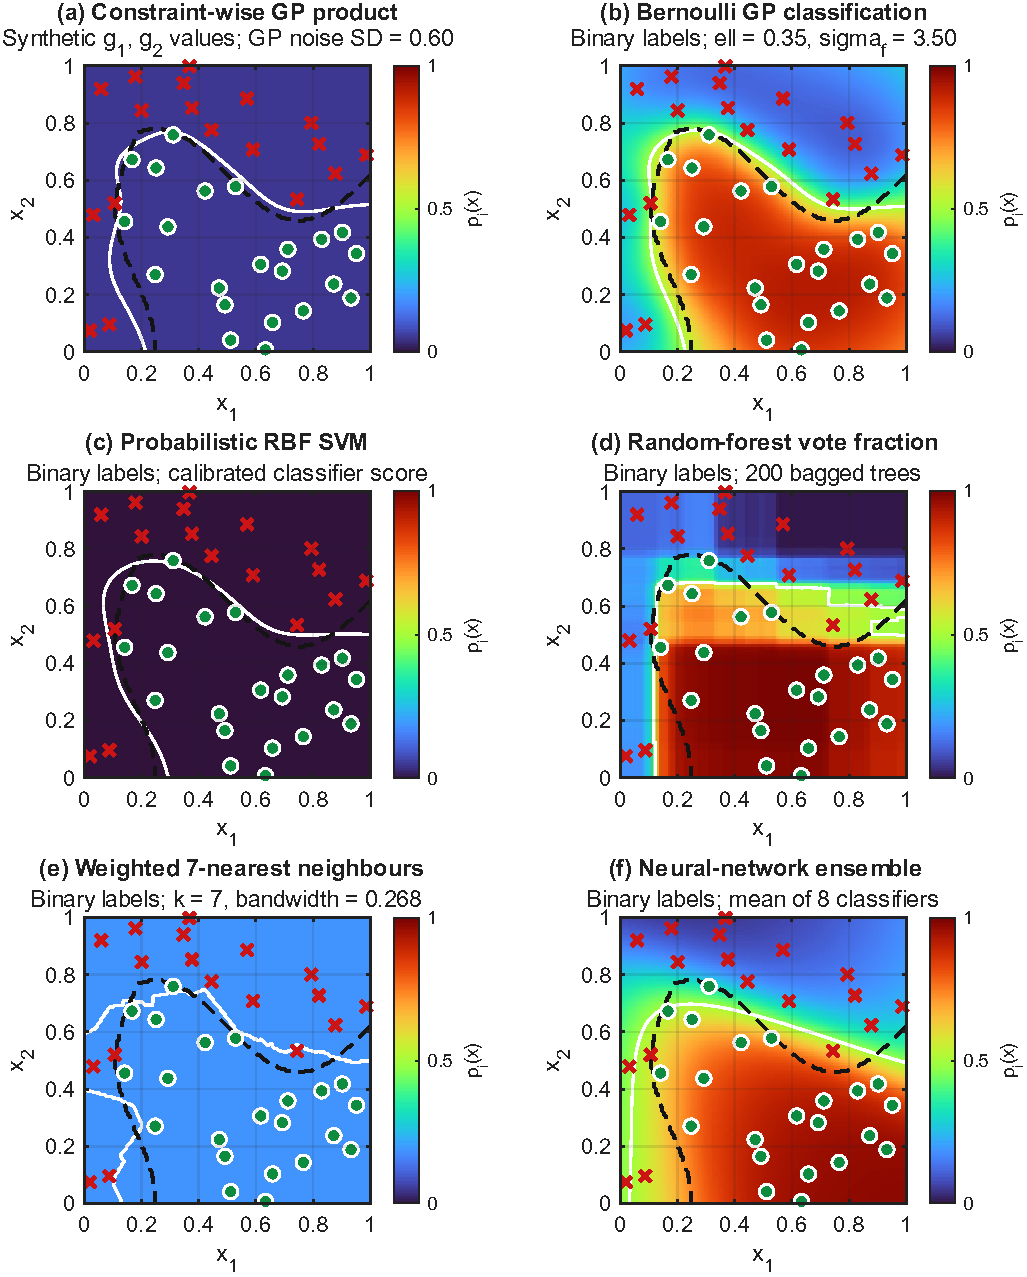
\includegraphics[width=\linewidth,height=0.75\textheight,keepaspectratio]
  {../introduction_pof_comparison/output/table1_pof_atlas.pdf}
\caption{Representative feasibility fields for the six methods in
Table~\ref{tab:binary-feasibility-methods}. Panel (a) receives synthetic
numerical constraint values; panels (b)--(f) receive the common aggregate
labels. \textit{Source:} Authors' calculations.}
\label{fig:table1-pof-atlas}
\end{figure}
\FloatBarrier

The fields exhibit distinct geometries under this fixed design. GP
classification, the support-vector construction, and the neural ensemble
produce smooth curved transitions, whereas the random forest and
nearest-neighbor methods retain more local or piecewise-constant structure.
The constraint-wise product forms a sharp boundary in this example and is the
only panel supplied with two numerical constraint-value data sets. Together, the panels
illustrate how the available information and modeling assumptions influence
field smoothness, locality, and anchor behavior.

Assessment therefore uses several complementary properties. Anchor consistency asks whether
\(p_i(\mathbf{x}_j)=y_j\) at an observed design; discrimination asks whether the
field ranks unseen feasible designs above violating designs; and calibration
asks whether stated probabilities agree with empirical frequencies.
Out-of-sample discrimination, score error or calibration where applicable,
and class-specific false rates describe different aspects of field quality.

A feasibility field can multiply an objective acquisition, impose a
feasibility threshold, filter candidates, drive feasibility discovery when no
feasible incumbent exists, or guide sampling near the estimated class boundary
\cite{gelbart2014unknown,basudhar2012svm,nardi2019hypermapper,
candelieri2021partially,tian2024boundary}. Classification surrogates can also
enter surrogate constraint-violation scores used to order direct-search
candidates without requiring a calibrated-probability interpretation, as in
treatments of binary, unrelaxable, and hidden constraints
\cite{audet2020binary}.

The present study receives one aggregate label per evaluated design, so
separate constraint-specific models require additional information. cTSEMO
instead maps the aggregate labels to exterior regression targets, fits a
locally scaled GP mean, clips the result to the unit interval, and snaps stored
anchors to their observed labels. The resulting \(p_i\) is used as an
operational feasibility score and is specified in
Section~\ref{sec:ctsemo-methodology}.

Figure~\ref{fig:gpc-ctsemo-pof-comparison} contrasts the graded class
probability produced by GPC with the clipped score and snapped anchors used by
cTSEMO. Both panels use identical observations, domain, and color limits. In
cTSEMO, \(-0.25\) and \(1.25\) are regression targets before clipping rather
than probability values. The comparison highlights two operational choices:
cTSEMO treats the labels as authoritative anchors and constructs an
inexpensive GP-regression field, whereas GPC retains a graded posterior class
probability. Their relative accuracy between observations depends on sampling
geometry and model settings.

\begin{figure}[H]
\centering
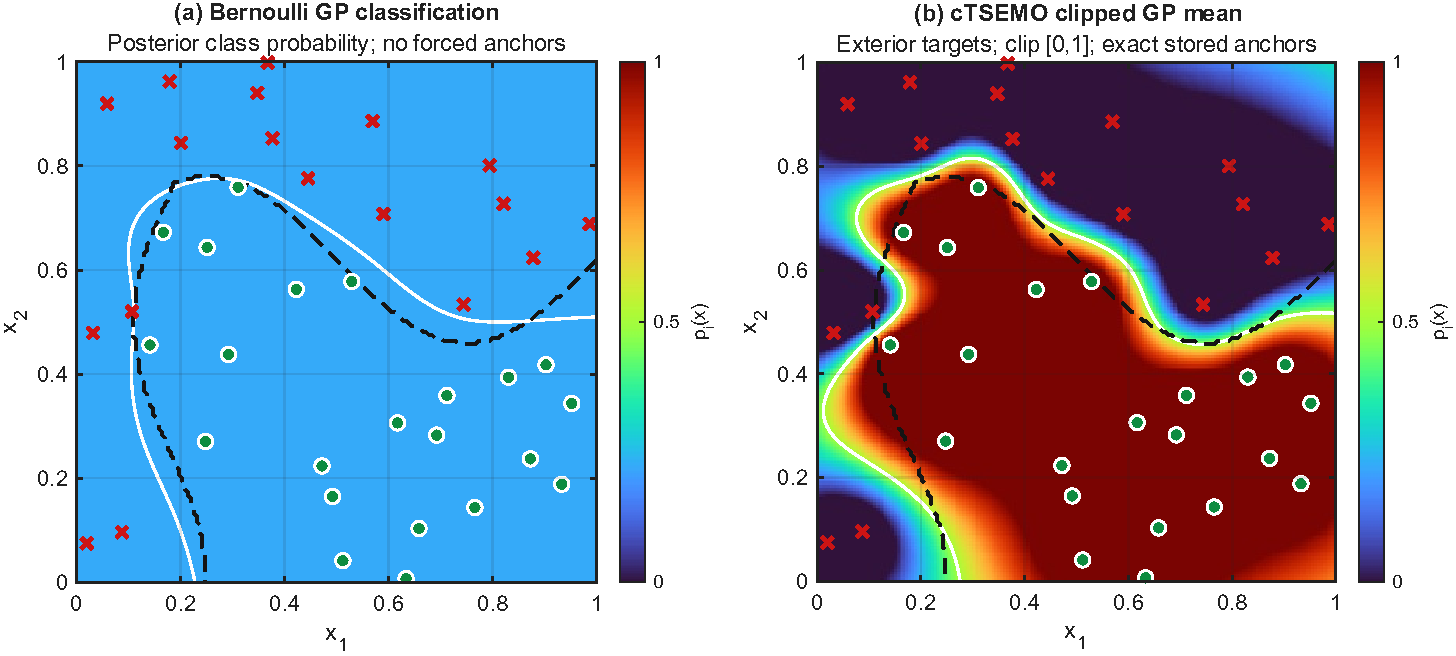
\includegraphics[width=\linewidth]
  {../introduction_pof_comparison/output/gpc_ctsemo_pof_comparison.pdf}
\caption{Bernoulli GP classification and the cTSEMO clipped GP-mean field
fitted to identical aggregate binary labels. \textit{Source:} Authors'
calculations.}
\label{fig:gpc-ctsemo-pof-comparison}
\end{figure}
\FloatBarrier

\subsection{Motivation, contributions, and scope of cTSEMO}
\label{sec:intro-contributions}

Extending TSEMO to aggregate binary-label constraints requires more than
selecting a feasibility surrogate.  The sequential decision system must
combine the feasibility field with sampled objective improvement, retain
diversity among candidate designs, and provide defined recovery paths when the initial design
contains no feasible observation, when no positive sampled HVI is detected in
the finite reference sets, or when a
candidate pool contains only unusable or previously evaluated designs.  An
overconfident field can suppress genuinely feasible but poorly explored
regions, whereas a broadly optimistic field can favor violating candidates.

Several ingredients of cTSEMO have relevant precedents. Heese and Bortz
combined binary feasibility classification, feasibility-weighted
Pareto-volume improvement, classifier-uncertainty sampling, repulsion, and
global acquisition search in constrained multiobjective Bayesian optimization
\cite{heese2021binary}. Other binary-label methods include
distance-controlled SVM-boundary refinement \cite{basudhar2012svm} and
mixed-variable classification-based search \cite{nardi2019hypermapper}. A
TSEMO-derived materials-design solver used two random-forest classifiers as
feasibility constraints within NSGA-II applied to Thompson-sampled objective
functions \cite{sattari2024physics}. Classifier-based active learning of
separately observed constraint boundaries has also been used in multiobjective
materials design
\cite{khatamsaz2022materials,khatamsaz2023entropy}. Feasibility-discovery policies
\cite{gelbart2014unknown,feliot2017constrained} and local penalization
\cite{gonzalez2016localpenalization} likewise predate the present work.

Building on these precedents, cTSEMO integrates objective Thompson sampling, a
deterministic clipped GP-mean feasibility score, direct genetic-algorithm
maximization of a scalar acquisition, and recorded discovery and recovery
states for one aggregate label per evaluated design. Relative to Heese and
Bortz, cTSEMO retains objective Thompson sampling and uses a deterministic
feasibility score. Relative to Sattari et al., it directly searches the scalar
acquisition instead of retaining sampled-Pareto candidate generation.

This paper makes three contributions:

\begin{enumerate}
  \item It specifies a TSEMO-derived workflow for two-objective
  expensive optimization with one aggregate feasible-or-violating label per
  evaluated design. The objective Gaussian-process, Thompson-sampling, and
  sampled-HVI principle is retained, while feasibility is handled through a
  separate, anchor-snapped clipped GP-mean channel within the larger search
  architecture.
  \item It defines a state-aware candidate-selection policy comprising bounded
  anti-clustering masks, a genetic-algorithm primary search, an independent
  same-acquisition challenger pool, hard duplicate exclusion, and explicit discovery or recovery
  transitions when no feasible observation exists, no positive sampled HVI is
  detected in the finite reference sets, or a
  candidate pool becomes unusable. Each transition and the source of the
  selected point are recorded for traceability.
  \item It characterizes feasibility-score discrimination, endpoint
  saturation, false classifications, challenger and fallback use, and observed
  feasibility-learning and recovery failure modes across the reported test
  suite.
\end{enumerate}

Evaluation is limited to two-objective constrained problems and focuses on
feasibility-field and candidate-selection behavior. Throughout the paper,
\(p_i\) denotes an uncalibrated operational feasibility score.

\section{cTSEMO methodology for aggregate binary-label constrained optimization}
\label{sec:ctsemo-methodology}

\subsection{Problem formulation and information boundary}

Let the bounded design domain be
\begin{equation}
  X=
  \left\{\mathbf{x}\in\R^d:
  \mathbf{x}^{\mathrm L}\leq\mathbf{x}\leq\mathbf{x}^{\mathrm U}\right\},
  \qquad \mathbf{x}^{\mathrm L}<\mathbf{x}^{\mathrm U}.
\end{equation}
The optimizer seeks the feasible Pareto set of two expensive minimization
objectives,
\begin{equation}
  \min_{\mathbf{x}\in X}\;
  \mathbf{f}(\mathbf{x})
  =
  \begin{bmatrix}f_1(\mathbf{x})&f_2(\mathbf{x})\end{bmatrix}^{\mathsf T},
  \qquad y(\mathbf{x})=1.
  \label{eq:problem}
\end{equation}
The observed constraint response is one aggregate label,
\begin{equation}
  y(\mathbf{x})=
  \begin{cases}
    1, & \mathbf{x}\text{ satisfies all requirements},\\
    0, & \mathbf{x}\text{ violates at least one requirement}.
  \end{cases}
  \label{eq:binary-label}
\end{equation}
If underlying margins \(g_r(\mathbf{x})\) exist, they are used only by the
benchmark oracle to calculate \(y(\mathbf{x})=\mathbb{I}
[\max_r g_r(\mathbf{x})\leq0]\).  They are not passed to the cTSEMO
feasibility model.  This distinction is essential when comparing against a
solver that receives continuous per-constraint margins.

The evaluated interface also requires finite values of both objectives at
every queried design, whether its aggregate label is feasible or violating.
It therefore does not cover crash or hidden constraints for which an objective
evaluation is unavailable after failure. Such failures terminate the evaluated
run and are checkpointed rather than converted silently into a binary label.

All surrogate calculations use normalized coordinates
\begin{equation}
  \mathbf{u}=
  \frac{\mathbf{x}-\mathbf{x}^{\mathrm L}}
       {\mathbf{x}^{\mathrm U}-\mathbf{x}^{\mathrm L}}
  \in[0,1]^d,
  \label{eq:normalization}
\end{equation}
where the quotient is componentwise.  The implementation stores physical
coordinates and bounds.  Units, when applicable, must be supplied by the
benchmark definition or accompanying artifact; they are not inferred by the
solver.

\subsection{Original TSEMO framework and cTSEMO modifications}

Bradford et al.'s MATLAB implementation performs the following sequence
\cite{bradford2018tsemo}: normalize the observations; fit one Gaussian
process per objective; draw one posterior function per objective; use a
multiobjective genetic algorithm to approximate the Pareto set of the sampled
functions; select a sampled-Pareto candidate with maximum HVI; evaluate the
expensive objectives; and update the observed Pareto set.

Table~\ref{tab:tsemo-ctsemo-changes} distinguishes principles retained from
TSEMO from the modifications introduced in cTSEMO. The implementation is a
modular derivative of this algorithmic sequence rather than a line-by-line
modification of the original source.

\begin{table}[H]
\centering
\caption{Relationship between the Bradford TSEMO framework and the cTSEMO
implementation. \textit{Source:} Bradford et al.~\cite{bradford2018tsemo} and
the authors' implementation.}
\label{tab:tsemo-ctsemo-changes}
\small
\begin{tabularx}{\linewidth}{@{}>{\raggedright\arraybackslash}p{0.22\linewidth}YY@{}}
\toprule
Component & Bradford TSEMO & cTSEMO modifications\\
\midrule
Objective models &
One Gaussian process and one posterior function draw per objective &
Retained for exactly two minimization objectives; fitting, sampling, and
random streams are separated into testable functions\\
Candidate utility &
HVI evaluated on candidates from sampled objective functions &
Retained as nonnegative sampled HVI \(H_k^{\mathrm{TS}}\); it is not expected
hypervolume improvement (EHVI)\\
Constraint information &
No aggregate binary-label feasibility field in the preserved TSEMO &
One anchor-snapped clipped GP mean \(p_i\) fitted to one aggregate label per
design\\
Candidate generation &
Sampled Pareto set approximated by a genetic algorithm &
Bounded genetic-algorithm (GA) maximization of the scalar constrained acquisition,
initialized from a seeded corner-augmented Latin-hypercube sampling (LHS) set
\cite{morris1995exploratory}; an independent LHS
challenger is evaluated by the same acquisition\\
Diversity &
Implicit through sampled Pareto search &
Optional bounded anti-clustering masks in normalized design and sampled
objective spaces\\
Degenerate states &
Not designed for an all-infeasible front or binary-score collapse &
Explicit no-feasible Phase I, no-detected-HVI/unusable-pool fallback, and hard
duplicate exclusion\\
Evidence &
Optimization and text logging in the original code &
Structured per-iteration component values, source labels, deterministic
component seeding, timings, checkpoints, and diagnostic exporters\\
\bottomrule
\end{tabularx}
\end{table}

\subsection{Operational feasibility field from aggregate binary labels}

\subsubsection{Exterior raw targets and prior mean}

At iteration \(k\), the feasibility data are
\(D_k=\{(\mathbf{u}_j,y_j)\}_{j=1}^{n_k}\).
For subsequent expressions,
\(\clip(a,l,u)=\min\{u,\max\{l,a\}\}\), for \(l\leq u\).
The label is mapped to an artificial continuous regression target
\begin{equation}
  z_j=z_-+(z_+-z_-)y_j,
  \qquad z_-=-0.25,\quad z_+=1.25
  \label{eq:raw-targets}
\end{equation}
by default. Both values are adjustable, subject to
\(0\leq m_0\leq1\), \(z_-<m_0<z_+\), \(z_-\leq0\), and
\(z_+\geq1\). The values \(-0.25\) and \(1.25\) are raw interpolation
targets; clipping and anchor snapping subsequently produce the final field
\(p_i\in[0,1]\) and its stored-anchor values.

The raw interpolant uses the constant prior mean \(m_0=0.5\). Exterior targets
separate the two classes from the clipping thresholds, and their separation
controls the extent of endpoint saturation. The target values are held fixed
in the reported experiments, which also report the resulting clipping
fractions.

The two one-class states use asymmetric search policies. When every observed
design is feasible, the implementation assigns \(p_i\equiv1\) and treats the
aggregate constraint as inactive until a violating label appears. When every
observation is violating, the fitted field is retained and the solver enters
the feasibility-discovery policy in Section~\ref{sec:phase-one}.

\subsubsection{Data-adaptive base length}

Consistent duplicate inputs are consolidated within a normalized tolerance of
\(10^{-12}\) before these geometric quantities are calculated; let
\(\bar n_k\) denote the resulting unique
count. Let \(r_j\) be the nearest-neighbor distance from
\(\mathbf{u}_j\) to any other unique observation and \(b_j\) the nearest
distance to an observation with the opposite label.  When both classes are
observed, the automatic base characteristic length is
\begin{equation}
  \ell_0=
  \clip\!\left(
  \sqrt{\operatorname{median}_j(r_j)\,
  \operatorname{median}_j(b_j)},\,
  \ell_{\min},\ell_{\max}\right).
  \label{eq:base-length}
\end{equation}
For a one-class data set with at least two unique points, the median
nearest-neighbor spacing replaces the opposite-label spacing. With one
unique point, the automatic value is \(0.25\) before applying the bounds.  The
implementation also permits a fixed positive \(\ell_0\). The bounds obey
\(0<\ell_{\min}\leq\ell_{\max}\); their evaluated values are
\((\ell_{\min},\ell_{\max})=(0.03,1.5)\) in the normalized domain.
The interval \([\ell_{\min},\ell_{\max}]\) clips only the automatically
calculated value; a manually supplied base length is required only to be
positive.

\subsubsection{Local enlargement in dense, pure infeasible regions}

The local length-scale rule increases characteristic length only where multiple
nearby infeasible labels provide mutually consistent support.  Let
\(I_-\) and \(I_+\) denote the infeasible and feasible
index sets among the consolidated anchors, with \(n_-=|I_-|\) and
\(n_+=|I_+|\), and let
\begin{equation}
  w_j(\mathbf{u})=
  \exp\!\left[-\frac{\|\mathbf{u}-\mathbf{u}_j\|_2^2}{2h_\rho^2}\right]
  \label{eq:density-weight}
\end{equation}
For \(\bar n_k\geq2\), the default bandwidth is
\begin{equation}
  h_\rho=\operatorname{median}_{j}
  d_{j,(k_{\mathrm{nn}})},\qquad
  k_{\mathrm{nn}}=\min\!\left(\bar n_k-1,
  \left\lceil\sqrt{\bar n_k}\right\rceil\right),
  \label{eq:density-bandwidth}
\end{equation}
where \(d_{j,(k_{\mathrm{nn}})}\) is the distance from training point \(j\) to its
\(k_{\mathrm{nn}}\)-th nearest other training point. A user-specified positive neighbor
count replaces \(\lceil\sqrt{\bar n_k}\rceil\) but is capped at
\(\bar n_k-1\); with fewer than two unique points, \(h_\rho=\ell_0\). The
implementation bounds \(h_\rho\) below by
\(\sqrt{\varepsilon_{\mathrm{mach}}}\), where
\(\varepsilon_{\mathrm{mach}}\) is double-precision machine epsilon. Define class sums
\(W_\pm(\mathbf{u})=\sum_{j\in I_\pm}w_j(\mathbf{u})\) and
the infeasible pair mass
\begin{equation}
  P_-(\mathbf{u})
  =\frac{1}{2}\left[
  W_-^2(\mathbf{u})-
  \sum_{j\in I_-}w_j^2(\mathbf{u})
  \right].
  \label{eq:pair-mass}
\end{equation}
A single infeasible observation cannot generate pair mass by itself. The implementation
evaluates \(P_-(\mathbf{u}_j)\) at all training points and sets
\(P_{\mathrm{ref}}\) to the median of values exceeding
\(\sqrt{\varepsilon_{\mathrm{mach}}}\). If none exist, the fallback is
\(P_{\mathrm{ref}}=1\).  The absolute support is
\begin{equation}
  a_-(\mathbf{u})
  =1-\exp\!\left[
  -\frac{\max(0,P_-(\mathbf{u}))}{P_{\mathrm{ref}}}
  \right].
  \label{eq:absolute-support}
\end{equation}
To keep the class comparison readable, define the two normalized local
densities as
\(\rho_-(\mathbf{u})=W_-(\mathbf{u})/\max(1,n_-)\) and
\(\rho_+(\mathbf{u})=W_+(\mathbf{u})/\max(1,n_+)\). Their contrast is
\begin{equation}
  c_-(\mathbf{u})=
  \left[
  \clip\!\left(
  \frac{\rho_-(\mathbf{u})-\rho_+(\mathbf{u})}
       {\rho_-(\mathbf{u})+\rho_+(\mathbf{u})+\varepsilon_{\rho}},
  0,1\right)
  \right]^{\eta}.
  \label{eq:purity}
\end{equation}
The internal values are \(\varepsilon_{\rho}=\varepsilon_{\mathrm{mach}}\)
and \(\eta=2\).  The bounded local support and characteristic length are
\begin{align}
  s_-(\mathbf{u})&=\clip[a_-(\mathbf{u})c_-(\mathbf{u}),0,1],
  \label{eq:local-support}\\
  \ell(\mathbf{u})&=\ell_0
  \min\!\left\{\lambda_{\max},1+\gamma s_-(\mathbf{u})\right\}.
  \label{eq:local-length}
\end{align}
Here \(\gamma\geq0\) controls local enlargement and
\(\lambda_{\max}\geq1\) prevents unbounded smoothing.  Setting
\(\gamma=0\) recovers a stationary covariance.  Feasible observations reduce
the purity term near a mixed-label interface, so the formulation is intended
to smooth dense infeasible interiors without deliberately straightening the
boundary.

\subsubsection{Dimension-generic nonstationary Mat\'ern covariance}

For two normalized points \(\mathbf{u}\) and \(\mathbf{v}\), let
\(\ell_u=\ell(\mathbf{u})\) and \(\ell_v=\ell(\mathbf{v})\).  The scalar
local-length Mat\'ern-\(3/2\) specialization of the
Paciorek--Schervish construction is \cite{paciorek2004nonstationary}
\begin{align}
  a(\mathbf{u},\mathbf{v})
  &=
  \left(
  \frac{2\ell_u\ell_v}{\ell_u^2+\ell_v^2}
  \right)^{d/2},
  \label{eq:ps-amplitude}\\
  q(\mathbf{u},\mathbf{v})
  &=
  \frac{2\|\mathbf{u}-\mathbf{v}\|_2^2}
       {\ell_u^2+\ell_v^2},
  \label{eq:ps-distance}\\
  k_{\mathrm{loc}}(\mathbf{u},\mathbf{v})
  &=
  a(\mathbf{u},\mathbf{v})
  \left(1+\sqrt{3q(\mathbf{u},\mathbf{v})}\right)
  \exp\!\left[-\sqrt{3q(\mathbf{u},\mathbf{v})}\right].
  \label{eq:local-matern}
\end{align}
The covariance has unit marginal variance,
\(k_{\mathrm{loc}}(\mathbf{u},\mathbf{u})=1\), and the construction applies to
arbitrary input dimension \(d\). For any fixed positive length field,
Equation~\eqref{eq:local-matern} is a valid positive-definite
Paciorek--Schervish covariance. In cTSEMO, the length field is constructed from
the observed labels, producing an empirical, label-dependent kernel. When
\(\ell_u\ne\ell_v\), the amplitude in
Equation~\eqref{eq:ps-amplitude} depends explicitly on \(d\). The dimensional
screen consequently combines sampling coverage, feasible prevalence, problem
geometry, and this dimension-dependent covariance construction.

\subsubsection{Tolerance-controlled interpolation, anchor snapping, and clipping}

After duplicate consolidation, let \(\bar{\mathbf{K}}_k\) be the
\(\bar n_k\times\bar n_k\) matrix with entries
\(k_{\mathrm{loc}}(\mathbf{u}_i,\mathbf{u}_j)\), let
\(\bar{\mathbf{z}}_k=[z_1,\ldots,z_{\bar n_k}]^{\mathsf T}\), and let
\(\mathbf{1}\in\mathbb{R}^{\bar n_k}\). Define
\([\bar{\mathbf{k}}_k(\mathbf{u})]_j=
k_{\mathrm{loc}}(\bar{\mathbf{u}}_j,\mathbf{u})\), where
\(\bar{\mathbf{u}}_j\) is the \(j\)th consolidated anchor. The coefficient
vector is obtained from
\begin{equation}
  \left(\bar{\mathbf{K}}_k+\delta_k\mathbf{I}\right)
  \boldsymbol{\alpha}_k
  =\bar{\mathbf{z}}_k-m_0\mathbf{1}.
  \label{eq:pof-system}
\end{equation}
The implementation first attempts \(\delta_k=0\) and increases numerical
jitter after either a Cholesky failure or an unsnapped anchor residual above
the configured tolerance.  An accepted solve is therefore
tolerance-controlled rather than algebraically exact when
\(\delta_k>0\). Conflicting labels at coincident inputs are rejected and
consistent duplicates are consolidated. The unsnapped raw mean is
\begin{equation}
  m_{\mathrm{raw},k}(\mathbf{u})
  =
  m_0+\bar{\mathbf{k}}_k(\mathbf{u})^{\mathsf T}
  \boldsymbol{\alpha}_k.
  \label{eq:raw-mean}
\end{equation}
The raw prediction is snapped only when a query exactly matches a stored
design. In that case it is replaced by the corresponding consolidated target
\(\bar z_j\); otherwise the value from Equation~\eqref{eq:raw-mean} is retained.
Consistent duplicates share one consolidated target, so this replacement is
unambiguous. Denote the resulting snapped raw mean by
\(\widetilde m_{\mathrm{raw},k}(\mathbf{u})\).
The operational feasibility field is
\begin{equation}
  p_{i,k}(\mathbf{u})
  =
  \clip\!\left(\widetilde m_{\mathrm{raw},k}(\mathbf{u}),0,1\right).
  \label{eq:clipped-pof}
\end{equation}
The unsnapped interpolation residual is retained as a numerical diagnostic,
while the snapped operational field satisfies
\begin{equation}
  p_{i,k}(\mathbf{u}_j)=y_j.
  \label{eq:anchor-property}
\end{equation}
Anchor snapping enforces label consistency at stored designs, and the hard
duplicate guard prevents their reselection. Predictions between anchors remain
determined by the fitted GP mean.

The feasibility model uses the fitted mean without drawing a random
feasibility function. For \(\alpha>0\), a clipped-zero region receives zero
ordinary acquisition. Such a region becomes accessible again when subsequent
refitting raises its score or when a recovery policy selects it.

\subsubsection{Interpretation and recommended diagnostics}
\label{sec:feasibility-field-diagnostics}

Clipping produces a bounded and ordered operational score with possible point
masses at zero and one. Its evaluation therefore combines:

\begin{itemize}
  \item exact anchor agreement and numerical conditioning;
  \item ranking, using area under the receiver-operating-characteristic curve
  (AUC) and average precision on fixed probe sets;
  \item magnitude-sensitive score error, using mean squared score error, and
  separate reliability diagnostics when probabilistic calibration is being
  assessed;
  \item false-feasible and false-infeasible rates at prespecified diagnostic
  thresholds;
  \item selected post-clipping point masses at 0 and 1, together with
  raw-mean extrema before clipping;
  \item conditional empirical cumulative distributions of the \emph{same}
  \(p_i\) field for truly feasible and truly infeasible probe subsets; and
  \item optimizer-level consequences under matched initial designs, seeds,
  budgets, and acquisitions.
\end{itemize}

The present study reports anchor agreement, AUC, mean squared score error,
thresholded false rates, saturation fractions, and observed optimizer
trajectories.

\subsection{Objective Thompson sampling and sampled hypervolume improvement}

\subsubsection{Objective surrogates}

For objective \(m\in\{1,2\}\), cTSEMO fits a Gaussian-process model to
normalized inputs and standardized objective values. Let
\(\mathbf y_{m,k}\) denote the vector of objective-\(m\) observations after
subtracting their current sample mean and dividing by their current sample
standard deviation. If that scale is nonfinite or no larger than
\(\sqrt{\varepsilon_{\mathrm{mach}}}\max(1,\max_j|f_m(\mathbf u_j)|)\), the
implementation substitutes unit scale. It then uses an anisotropic Mat\'ern-\(3/2\)
covariance,
\begin{equation}
  k_m(\mathbf{u},\mathbf{v})=
  \sigma_{f,m}^2
  \left(1+\sqrt{3r_m^2}\right)
  \exp\!\left(-\sqrt{3r_m^2}\right),
  \quad
  r_m^2=\sum_{r=1}^{d}
  \frac{(u_r-v_r)^2}{\ell_{m,r}^2}.
  \label{eq:objective-kernel}
\end{equation}
where \(\sigma_{f,m}>0\) is the signal standard deviation and
\(\ell_{m,r}>0\) is the characteristic length in coordinate \(r\).
Once at least one feasible observation exists, each objective GP uses all
current objective observations, including those at violating designs;
feasibility restricts the front used for HVI rather than the GP training set.
Before the first feasible observation, objective fitting and drawing are
skipped. Hyperparameters are optimized using the observed objective data when
possible; constant objectives and data sets with fewer than two observations
bypass that optimization. One
approximate posterior function \(\widetilde f_{m,k}\) is then drawn for each
objective. The implementation uses Mat\'ern spectral features in the TSEMO
tradition \cite{bradford2018tsemo}, followed by an exact-kernel conditioning
correction through Matheron's rule \cite{wilson2020pathwise}. Let
\(\mathbf{K}_{f,m,k}\) be the latent covariance at the observations,
\begin{equation}
  \mathbf{K}_{y,m,k}
  =
  \mathbf{K}_{f,m,k}
  +\sigma_{n,m}^2\mathbf{I}
  +\delta_{m,k}\mathbf{I},
  \label{eq:objective-observation-covariance}
\end{equation}
where \(\sigma_{n,m}>0\) is the fitted observation-noise standard deviation
(the implementation enforces a lower bound of \(10^{-8}\)),
\(\delta_{m,k}\geq0\) is numerical jitter, and
\(\mathbf{k}_{f,m,k}(\mathbf{u})\) is the latent cross-covariance. If
\(\widetilde f_{m,k}^{\,0}\) is a finite-feature prior draw and
\(\boldsymbol{\epsilon}_{m,k}^{\,0}\sim
\mathcal{N}(\mathbf{0},\sigma_{n,m}^2\mathbf{I})\) is an observation-noise
draw independent of the finite-feature prior draw, let
\(\widetilde{\mathbf f}_{m,k}^{\,0}\) denote the prior draw
evaluated at the training inputs. The conditioned sample is
\nopagebreak[4]
\begin{equation}
  \widetilde f_{m,k}(\mathbf{u})
  =
  \widetilde f_{m,k}^{\,0}(\mathbf{u})
  +\mathbf{k}_{f,m,k}(\mathbf{u})^{\mathsf T}
  \mathbf{K}_{y,m,k}^{-1}
  \left[
  \mathbf{y}_{m,k}
  -\widetilde{\mathbf f}_{m,k}^{\,0}
  -\boldsymbol{\epsilon}_{m,k}^{\,0}
  \right].
  \label{eq:matheron-draw}
\end{equation}
Because the prior draw uses finitely many spectral features, this remains an
approximate posterior function draw even though its correction uses the exact
fitted kernel matrices.
Component-specific random streams are isolated and derived deterministically
from the stored run seed and iteration index. Objective draws, candidate-pool
generation, primary GA search, and diagnostic resampling therefore remain
reproducible without sharing random-number-generator state. Full logging also
retains the objective-draw payloads and GA seed.

\subsubsection{Sampled hypervolume improvement}

Let \(\mathbf f_k^z(\mathbf u_j)\) denote the two-objective vector after each
component has been standardized using all current observations, and let
\(P_k^{F,z}\) be the nondominated standardized objective vectors
among the observed \emph{feasible} designs. The iteration uses a dynamic
reference vector \(\mathbf{r}_k^{A}\) in the same coordinates:
\begin{equation}
  \mathbf{r}_k^{A}
  =
  \mathbf{y}_{k}^{\max}
  +
  \max\!\left[
  0.1(\mathbf{y}_{k}^{\max}-\mathbf{y}_{k}^{\min}),
  0.1\max(1,|\mathbf{y}_{k}^{\max}|)
  \right],
  \label{eq:acquisition-reference}
\end{equation}
where \(\mathbf y_k^{\min}\) and \(\mathbf y_k^{\max}\) are the componentwise
extrema of the observed feasible objective vectors in these standardized
coordinates, and all vector operations are componentwise. The utility of a
candidate is
\begin{equation}
  H_k^{\mathrm{TS}}(\mathbf{u})
  =
  \max\!\left\{0,\,
  \HV\!\left(
  P_k^{F,z}\cup
  \{\widetilde{\mathbf f}_k(\mathbf{u})\};\mathbf{r}_k^{A}
  \right)
  -
  \HV\!\left(P_k^{F,z};\mathbf{r}_k^{A}\right)
  \right\},
  \label{eq:sampled-hvi}
\end{equation}
where
\(\widetilde{\mathbf f}_k=
[\widetilde f_{1,k},\widetilde f_{2,k}]^{\mathsf T}\).
For this two-objective minimization problem,
\(\HV(P;\mathbf r)\) is the area dominated by the nondominated set
\(P\) and bounded above by the reference vector \(\mathbf r\); a point
that is not componentwise below \(\mathbf r\) contributes zero area.
This is HVI under one Thompson realization.  It is not an expectation over
the objective posterior and is therefore not EHVI.

The reference vector in Equation~\eqref{eq:acquisition-reference} is
iteration dependent and is used only to define the acquisition. Cross-run
hypervolume comparisons require a fixed reference vector, specified before
analysis and shared across solvers and seeds. Run-specific or solver-specific
post hoc reference vectors are unsuitable for such comparisons.

\subsection{Acquisition, GA primary search, challenger, and recovery policies}

\subsubsection{Anti-clustering masks}

The masks reduce immediate reselection near evaluated designs. The codomain
mask additionally downweights a candidate when its current Thompson-sampled
objective vector lies near an observed standardized objective vector. Let
\begin{equation}
  \varphi(t)=
  \begin{cases}
    (1-t)^4(4t+1),&0\leq t<1,\\
    0,&t\geq1
  \end{cases}
  \label{eq:wendland-bump}
\end{equation}
be a compact bump \cite{wendland1995compact}. Using Euclidean distance in the
normalized design coordinates and in the standardized two-objective
coordinates, the masks are
\begin{align}
  M_{X,k}(\mathbf{u})
  &=
  m_X+(1-m_X)\!\left[
  1-\max_{j\leq n_k}
  \varphi\!\left(
  \frac{\|\mathbf{u}-\mathbf{u}_j\|_2}{r_X}
  \right)
  \right],
  \label{eq:design-mask}\\
  M_{Y,k}(\mathbf{u})
  &=
  m_Y+(1-m_Y)\!\left[
  1-\max_{j\leq n_k}
  \varphi\!\left(
  \frac{\|\widetilde{\mathbf f}_k(\mathbf{u})
  -\mathbf{f}_k^z(\mathbf{u}_j)\|_2}{r_Y}
  \right)
  \right].
  \label{eq:objective-mask}
\end{align}
The compact Wendland function is used solely to construct the anti-clustering
masks. The floors \(m_X,m_Y\in[0,1]\) and radii \(r_X,r_Y>0\) are configurable.
Hard design duplicates receive \(M_{X,k}=0\) independently of the optional
soft mask.

\subsubsection{Main acquisition}

Before continuous acquisition search, cTSEMO constructs a finite primary seed
set \(S_k\) and an independent challenger set
\(C_k\).  Let
\(H_k^+=\{H_k^{\mathrm{TS}}(\mathbf{u}):
\mathbf{u}\in S_k\cup C_k,\,
H_k^{\mathrm{TS}}(\mathbf{u})>h_{\min}\}\), where \(h_{\min}=10^{-12}\) by
default.  When this set is nonempty, the background term is
\begin{equation}
  \epsilon_k=
  \max\!\left\{\epsilon_0,\,
  \beta_\epsilon
  Q_{q_\epsilon}\!\left(H_k^+\right)\right\},
  \label{eq:adaptive-background}
\end{equation}
where \(Q_q\) is the linearly interpolated empirical quantile.  The defaults
are \(\epsilon_0=0\), \(\beta_\epsilon=0.25\), and
\(q_\epsilon=0.25\), with \(h_{\min},\epsilon_0,\beta_\epsilon\geq0\) and
\(q_\epsilon\in[0,1]\). The threshold \(h_{\min}\) filters the samples used
to estimate this background quantile. When \(H_k^+\) is empty,
\(\epsilon_k=\epsilon_0\); ordinary selection remains eligible if either
finite reference set contains positive HVI. This value is calculated once from the reference sets
and then held fixed during the genetic-algorithm search and final
primary--challenger comparison.  Freezing \(\epsilon_k\) prevents the scalar
objective presented to the genetic algorithm from changing merely because a
different population batch is being evaluated.  The defining acquisition is
\begin{equation}
  A_k(\mathbf{u})=
  \left[H_k^{\mathrm{TS}}(\mathbf{u})+\epsilon_k\right]
  p_{i,k}(\mathbf{u})^{\alpha}
  M_{X,k}(\mathbf{u})M_{Y,k}(\mathbf{u}),
  \qquad \alpha=1\ \text{by default}.
  \label{eq:main-acquisition}
\end{equation}
The implementation permits \(\alpha\geq0\), with the convention
\(p_{i,k}^{\,0}=1\), including at \(p_{i,k}=0\).
The finite reference-set screen has three outcomes. Positive HVI permits the
ordinary search, including values in \((0,h_{\min}]\) that are omitted from the
background quantile. Absence of positive HVI records a no-positive-HVI status
and requests recovery. Positive HVI accompanied by zero acquisition values
after feasibility weighting or masking records a no-positive-acquisition
status and also requests recovery. Candidate-generation, finite-value, and
low-acquisition guards remain applicable.

\subsubsection{GA-optimized primary acquisition and LHS challenger}

The primary reference set \(S_k\) contains 1,024 points in total. In
dimensions not exceeding the configured corner limit, eligible hyperrectangle
corners occupy rows of this set and a seeded Latin-hypercube design fills the
remainder. The challenger set \(C_k\) is generated from a separate seeded
Latin-hypercube stream and contains no added corners.  Evaluated designs are
excluded from both sets within a normalized tolerance, and exact overlaps are
removed. The evaluated default scores the complete primary and challenger
sets. All remaining reference points are scored once to define \(\epsilon_k\)
in Equation~\eqref{eq:adaptive-background}.

The highest-scoring primary seed points initialize a bounded genetic
algorithm, which seeks the continuous-domain primary proposal
\begin{equation}
  \widehat{\mathbf{u}}_k^{G}
  \;\approx\;
  \arg\max_{\mathbf{u}\in[0,1]^d} A_k(\mathbf{u}).
  \label{eq:primary-ga-search}
\end{equation}
A finite genetic-algorithm run approximates this maximum. The implementation
default uses population size 80,
elite count 2, at most 120 generations, a 30-generation stall limit, and
function tolerance \(10^{-8}\). Serial execution is the deterministic default,
and the search requires MATLAB Global Optimization Toolbox. A failed GA
terminates the iteration.
After the GA returns, its raw proposal is scored and compared with the best
primary seed; the retained primary point is never permitted to score below
that seed.

The independent LHS challenger is not locally refined.  Its best point is
\begin{equation}
  \widehat{\mathbf{u}}_k^{C}
  =\arg\max_{\mathbf{u}\in C_k}A_k(\mathbf{u}).
  \label{eq:challenger-search}
\end{equation}
The retained primary point and every point in \(C_k\) are then rescored with
the same Thompson draws, frozen \(\epsilon_k\), feasibility-score exponent,
and masks. The challenger proposal is the maximum of this verified challenger
batch. Subject to the hard duplicate and fallback guards, the ordinary
selection is
\begin{equation}
  \mathbf{u}_{k+1}
  =\arg\max_{\mathbf{u}\in
  \{\widehat{\mathbf{u}}_k^{G},\widehat{\mathbf{u}}_k^{C}\}}
  A_k(\mathbf{u}),
  \label{eq:primary-challenger-arbitration}
\end{equation}
with ties assigned to the primary proposal.
The challenger receives no novelty
blend, Pareto-gap score, endpoint bonus, or source-specific multiplier.  It is
an independent coverage check on the same acquisition function, whereas
the primary is its genetic-algorithm maximizer.  The seed-set maximum, genetic
algorithm termination information, both final source-specific values, and the
winning source are retained in the iteration record.

\subsubsection{Phase I when no feasible point has been observed}
\label{sec:phase-one}

If \(\sum_{j=1}^{n_k}y_j=0\), the feasible Pareto set is empty and sampled HVI
is undefined as an ordinary constrained improvement signal.  cTSEMO skips
objective-GP fitting and enters an objective-independent
feasibility-discovery phase. Define the normalized distance from the evaluated
designs as
\begin{equation}
  d_k(\mathbf{u})=
  \min_{j\leq n_k}\|\mathbf{u}-\mathbf{u}_j\|_2
  \label{eq:min-distance}
\end{equation}
and the bounded novelty as
\begin{equation}
  \nu_k(\mathbf{u})
  =
  \left[
  1-\exp\!\left(-\frac{d_k(\mathbf{u})}{s_D}\right)
  \right]^{\lambda_D}.
  \label{eq:fallback-novelty}
\end{equation}
where \(s_D>0\) and \(\lambda_D\geq0\); when \(\lambda_D=0\), the
implementation uses \(\nu_k(\mathbf{u})=1\).
Phase I ranks the fallback score in
Equation~\eqref{eq:fallback-score} over the current finite admissible
candidate set. When clipping makes \(p_i=0\) everywhere,
the feasibility-score floor is constant and, for \(\lambda_D>0\), the rule
reduces to maximin-like novelty; for \(\lambda_D=0\), all admissible candidates
tie under this score.
The first feasible evaluation establishes the constrained reference front and
activates Equation~\eqref{eq:main-acquisition}. During Phase I, the stored selection source is \texttt{fallback}, with
reason \texttt{noFeasibleObservation} and state
\texttt{feasibilityDiscovery}.

\subsubsection{No-detected-HVI and unusable-pool fallback}

The ordinary recovery score retains a feasibility floor while rewarding
distance from existing evaluations:
\begin{equation}
  S_{\mathrm{fb},k}(\mathbf{u})
  =
  \max\!\left[p_{i,k}(\mathbf{u}),p_{\mathrm{floor}}\right]
  \nu_k(\mathbf{u}).
  \label{eq:fallback-score}
\end{equation}
The default safeguard settings are \(p_{\mathrm{floor}}=0.60\),
\(s_D=0.10\), and \(\lambda_D=1\), with
\(p_{\mathrm{floor}}\in[0,1]\).
Let \(B_k\) denote the finite set of admissible candidate rows available to a
given recovery call. Both Phase I and ordinary recovery select
\[
  \mathbf{u}_{k+1}\in
  \arg\max_{\mathbf{u}\in B_k}S_{\mathrm{fb},k}(\mathbf{u});
\]
the fallback score is not optimized continuously by the primary GA.
Individual nonfinite rows are discarded and do not trigger recovery while a
finite positive score remains. With fallback enabled, recovery is invoked by
a no-positive-HVI or no-positive-acquisition status, or when the verified
primary--challenger maximum satisfies
\(\max A_k\leq\tau_{\mathrm{fb}}\), with
\(\tau_{\mathrm{fb}}=10^{-12}\) by default. Phase I, a recognized
candidate-generation failure, or the absence of a finite verified maximum
forces recovery independently of that option. If no admissible row remains,
the solver generates one deterministic emergency pool and repeats the finite
ranking once; failure of that pool terminates the iteration. Each trigger and
selected source are retained in the iteration record.

The generated seed, challenger, and emergency sets are prefiltered using an
\(\ell_\infty\) distance tolerance of \(10^{-9}\) in normalized coordinates.
During acquisition scoring, including evaluation of a continuous GA proposal,
the hard-duplicate flag instead uses Euclidean distance with the same
normalized tolerance. The soft design-space mask in
Equation~\eqref{eq:design-mask} also uses Euclidean distance, with its
separate configurable radius \(r_X\). These operations provide pool
prefiltering, exact duplicate exclusion, and soft repulsion, respectively. If an objective or constraint
evaluation errors or returns an invalid value, cTSEMO writes an
evaluation-failure checkpoint when an output directory is active, terminates
the run, and does not append or count that point as a completed evaluation.

\subsubsection{Algorithm flowchart}

Figure~\ref{fig:ctsemo-flowchart} follows the vertical structure of the
original TSEMO flowchart and shows the default fallback-enabled workflow. White
nodes denote retained TSEMO operations, blue nodes denote cTSEMO additions or
modifications, blue text inside a white node marks an addition to a retained
operation, and the dashed amber node denotes Phase I and recovery behavior. Implementation
tolerances, random-stream handling, and failure logging remain specified in the
preceding subsections and are intentionally omitted from the diagram.

\begin{figure}[p]
\centering
\resizebox{!}{0.87\textheight}{%
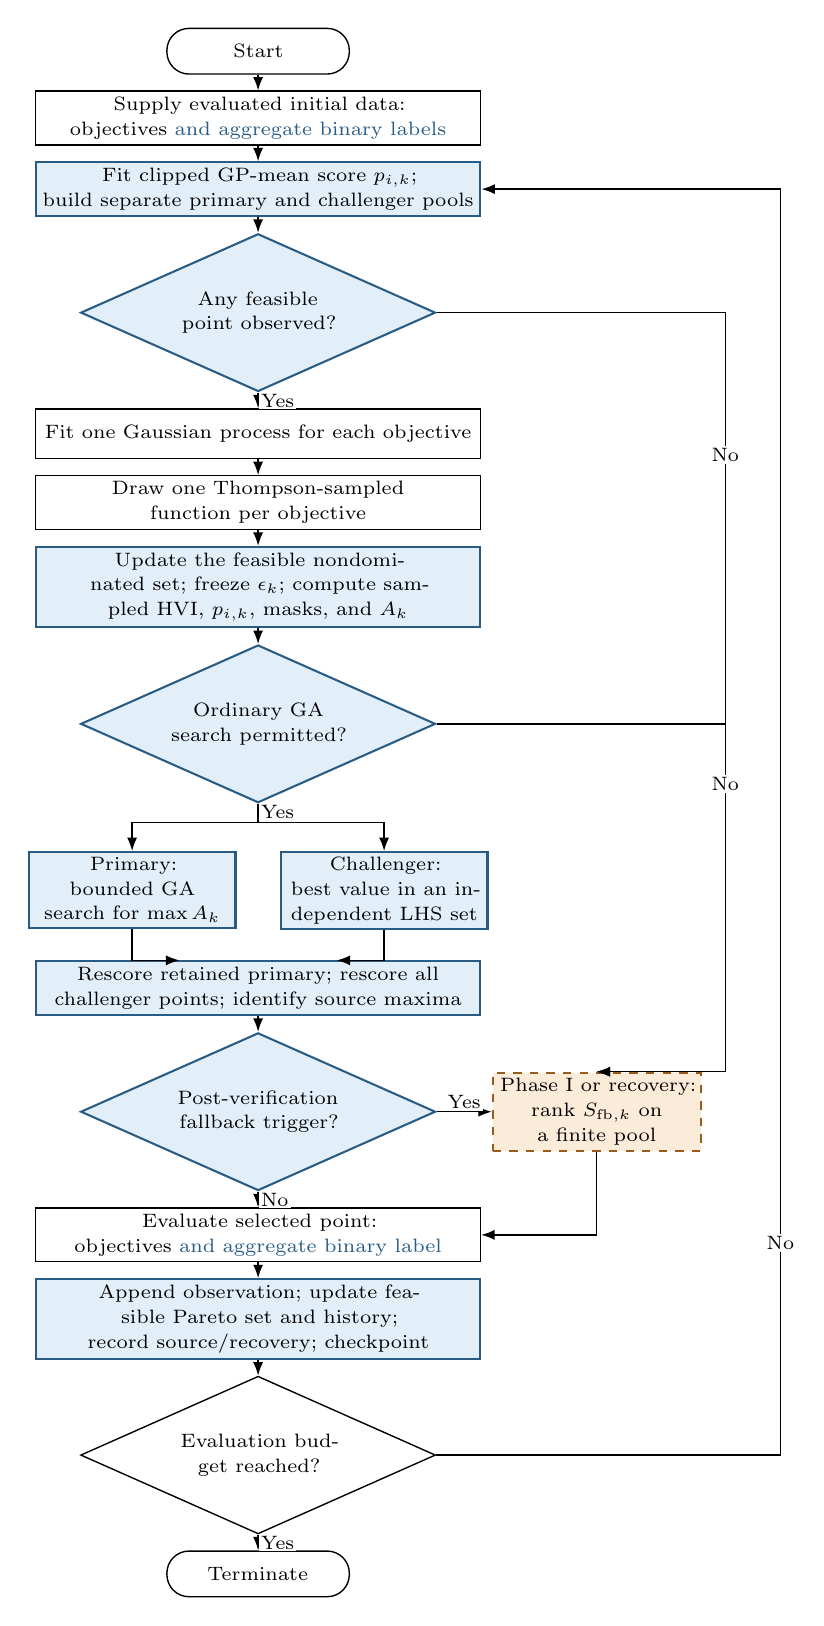
\begin{tikzpicture}[
  font=\footnotesize,
  node distance=2.0mm and 6mm,
  flowarrow/.style={-{Latex[length=1.7mm]},line width=0.5pt},
  tsemo/.style={draw=black,line width=0.5pt,align=center,text width=55mm,
    minimum height=6.3mm,inner sep=2.1pt},
  ctadd/.style={tsemo,draw=ctblueedge,fill=ctbluefill,line width=0.75pt},
  recover/.style={draw=ctamberedge,fill=ctamberfill,dashed,line width=0.75pt,
    align=center,text width=25mm,minimum height=7mm,inner sep=2pt},
  terminal/.style={draw=black,rounded corners=8pt,line width=0.5pt,
    align=center,text width=21mm,minimum height=5.8mm},
  decision/.style={diamond,aspect=2.25,draw=black,line width=0.5pt,
    align=center,text width=31mm,inner sep=0.9pt},
  ctdecision/.style={decision,draw=ctblueedge,fill=ctbluefill,line width=0.75pt},
  ctsmall/.style={draw=ctblueedge,fill=ctbluefill,line width=0.75pt,
    align=center,text width=25mm,minimum height=7mm,inner sep=1.8pt},
  branchlabel/.style={font=\scriptsize,fill=white,inner sep=0.8pt}
]
\node[terminal] (start) {Start};
\node[tsemo,below=of start] (initial) {Supply evaluated initial data:\\objectives
  \textcolor{ctblueedge}{and aggregate binary labels}};
\node[ctadd,below=of initial] (pof) {Fit clipped GP-mean score \(p_{i,k}\);\\
  build separate primary and \mbox{challenger} pools};
\node[ctdecision,below=of pof] (feasible) {Any feasible point observed?};
\node[tsemo,below=of feasible] (objectivegp) {Fit one Gaussian process for each objective};
\node[tsemo,below=of objectivegp] (draws) {Draw one Thompson-sampled function per objective};
\node[ctadd,below=of draws] (acquisition) {Update the feasible nondominated set;
  freeze \(\epsilon_k\); compute sampled HVI, \(p_{i,k}\), masks, and \(A_k\)};
\node[ctdecision,below=of acquisition] (ordinary) {Ordinary GA search
  permitted?};
\node[ctsmall,below=6mm of ordinary,xshift=-16mm] (primary) {Primary:\\
  bounded GA search for \(\max A_k\)};
\node[ctsmall,below=6mm of ordinary,xshift=16mm] (challenger) {Challenger:\\
  best value in an independent LHS set};
\node[ctadd,below=4mm of primary.south,xshift=16mm] (arbitrate) {Rescore retained
  primary; rescore all \mbox{challenger} points; identify source maxima};
\node[ctdecision,below=of arbitrate] (verify) {Post-verification fallback
  trigger?};
\node[recover,right=7mm of verify] (recovery) {Phase I or recovery:\\
  rank \(S_{\mathrm{fb},k}\) on a finite pool};
\node[tsemo,below=of verify] (evaluate) {Evaluate selected point:\\objectives
  \textcolor{ctblueedge}{and aggregate binary label}};
\node[ctadd,below=of evaluate] (update) {Append observation; update feasible
  Pareto set and history; record source/recovery; checkpoint};
\node[decision,below=of update] (budget) {Evaluation budget reached?};
\node[terminal,below=of budget] (stop) {Terminate};

\draw[flowarrow] (start)--(initial);
\draw[flowarrow] (initial)--(pof);
\draw[flowarrow] (pof)--(feasible);
\draw[flowarrow] (feasible)--node[branchlabel,right]{Yes}(objectivegp);
\draw[flowarrow] (objectivegp)--(draws);
\draw[flowarrow] (draws)--(acquisition);
\draw[flowarrow] (acquisition)--(ordinary);
\coordinate (ordinaryfork) at ($(ordinary.south)+(0,-2.4mm)$);
\draw[line width=0.5pt] (ordinary.south)--node[branchlabel,right,pos=0.45]{Yes}(ordinaryfork);
\draw[flowarrow] (ordinaryfork)-|(primary.north);
\draw[flowarrow] (ordinaryfork)-|(challenger.north);
\draw[flowarrow] (primary.south)|-([xshift=-10mm]arbitrate.north);
\draw[flowarrow] (challenger.south)|-([xshift=10mm]arbitrate.north);
\draw[flowarrow] (arbitrate)--(verify);
\draw[flowarrow] (verify)--node[branchlabel,right]{No}(evaluate);
\draw[flowarrow] (verify.east)--node[branchlabel,above]{Yes}(recovery.west);
\draw[flowarrow] (recovery.south)|-(evaluate.east);
\coordinate (discoverylane) at ($(recovery.east)+(3mm,0)$);
\draw[flowarrow] (feasible.east)--(discoverylane|-feasible.east)|-
  node[branchlabel,pos=0.10,above]{No}(recovery.north);
\draw[flowarrow] (ordinary.east)--(discoverylane|-ordinary.east)|-
  node[branchlabel,pos=0.10,above]{No}(recovery.north);
\draw[flowarrow] (evaluate)--(update);
\draw[flowarrow] (update)--(budget);
\draw[flowarrow] (budget)--node[branchlabel,right]{Yes}(stop);
\coordinate (looplane) at ($(recovery.east)+(10mm,0)$);
\draw[flowarrow] (budget.east)--(looplane|-budget.east)|-
  node[branchlabel,pos=0.08,above]{No}(pof.east);
\end{tikzpicture}
}
\caption{cTSEMO workflow relative to the original TSEMO iteration. Blue nodes
denote additions or modifications; the dashed amber node denotes Phase I and
recovery. \textit{Source:} Bradford et al.~\cite{bradford2018tsemo} and the
authors' implementation.}
\label{fig:ctsemo-flowchart}
\end{figure}
\FloatBarrier

\section{Implementation, logging, and computational cost}

\subsection{MATLAB implementation structure}

The software interface is
\begin{verbatim}
options = cTSEMOOptions(overrides);
result  = cTSEMO(f, g, X0, Y0, C0, lb, ub, options);
\end{verbatim}
The evaluated scope is two minimization objectives, bounded continuous design
variables, one aggregate binary feasibility response, one new point per
iteration, and deterministic labels. The implementation separates input
validation, objective modeling, objective Thompson draws, feasibility-field fitting,
candidate generation, acquisition evaluation, selection, Pareto updates,
checkpointing, diagnostics, benchmarks, and tests.  The vendored Bradford
snapshot is retained for provenance and is separate from the cTSEMO entry point.

The returned result structure contains metadata, normalized and physical problem
information, options, complete evaluated data, per-iteration records, and the
feasible Pareto set. Unknown option fields raise validation errors. Numeric
\(0/1\) labels require an explicit encoding to identify which value denotes
feasibility.

\subsection{Implementation defaults}

Table~\ref{tab:release-defaults} records the configuration used in the
experiments. Evaluation budgets are benchmark-specific overrides and are not
part of this table.

\begin{table}[H]
\centering
\caption{Selected defaults in the evaluated cTSEMO configuration.}
\label{tab:release-defaults}
\small
\begin{tabularx}{\linewidth}{@{}>{\raggedright\arraybackslash}p{0.29\linewidth}Y>{\raggedright\arraybackslash}p{0.24\linewidth}@{}}
\toprule
Component & Setting & Default value\\
\midrule
Primary search & Reference points; GA population; elite count &
1,024; 80; 2\\
Challenger & Independent LHS points & 512\\
Primary GA termination & Maximum generations; stall limit; function tolerance &
120; 30; \(10^{-8}\)\\
Primary GA execution & Parallel evaluation; failure policy &
disabled; \texttt{error} (terminates the run)\\
Objective Thompson draw & Covariance; spectral features &
Mat\'ern-\(3/2\); 256 per objective\\
Binary feasibility field & Raw targets; prior mean &
\(-0.25,\ 1.25\); \(0.50\)\\
Local feasibility length & Strength; configured maximum multiplier &
\(1.0;\ 3.0\) (effective maximum \(2.0\))\\
Main acquisition & \(p_i\) exponent; background-quantile HVI cutoff &
\(1.0;\ 10^{-12}\)\\
Adaptive background & Quantile; scale; fixed floor &
\(0.25;\ 0.25;\ 0\)\\
Design-space mask & Radius; floor & \(0.02;\ 0\)\\
Sampled-objective mask & Radius; floor & \(0.05;\ 0\)\\
Fallback & Feasibility floor; distance scale; exponent &
\(0.60;\ 0.10;\ 1.0\)\\
Fallback trigger & Enabled; verified-acquisition tolerance
\(\tau_{\mathrm{fb}}\) & true; \(10^{-12}\)\\
Feasibility anchors & Consolidation tolerance & \(10^{-12}\)\\
Selection safeguards & Corner limit; duplicate tolerance &
\(d\leq4;\ 10^{-9}\)\\
\bottomrule
\end{tabularx}
\parbox{\linewidth}{\footnotesize\textit{Source:} Authors' implementation.}
\end{table}

\subsection{Run records}

Each completed iteration records the physical and normalized design,
objectives, aggregate label, selection source, acquisition components,
fallback state, random seeds retained by the implementation, timing, and the
updated feasible Pareto set. Campaign-level records preserve the initial
designs, solver options, benchmark identifiers, validation summaries, and
source-version records. Offline diagnostic reconstructions are stored separately
from the acquisition-time quantities, preserving their distinct information
sets.

\subsection{Complexity}

Let \(n\) be the number of evaluated designs, \(d\) the number of design
variables, \(R\) the number of spectral features per objective,
\(N_P\) and \(N_C\) the primary-seed and challenger counts, \(Q_G\) the
number of acquisition evaluations performed by the genetic algorithm, and
\(E\) the number of likelihood evaluations used by one objective
hyperparameter search.  Each
likelihood evaluation constructs a dense anisotropic covariance and factors
it, giving approximately \(O(E(n^3+n^2d))\) time per objective fit.  The
single dense feasibility-field solve costs \(O(n^3)\), with \(O(n^2)\)
storage; density/support construction and anchor cross-covariance add
\(O(n^2d)\) during fitting. The all-feasible shortcut avoids this solve.

For each objective, finite-feature draw construction costs approximately
\(O(nRd+n^2)\). Let \(Q_G\) denote the objective/acquisition evaluations made
within the GA, excluding the constant number of returned-point verification
calls. Objective Thompson functions are evaluated at approximately
\[
  Q_{\mathrm{TS}}=N_P+N_C+Q_G+O(1)
\]
points, while PoF, masks, HVI, and the final challenger rescoring require
\[
  Q_A=N_P+2N_C+Q_G+O(1)
\]
pointwise acquisition evaluations. Their spectral-prior and exact
cross-covariance costs are approximately
\(O(Q_{\mathrm{TS}}Rd)\) and \(O(Q_{\mathrm{TS}}nd)\), respectively.
For a feasible front of size \(F_k\), direct two-objective HVI integration
adds \(O(Q_A F_k)\) after front construction. Feasibility-score prediction
and design- and objective-space distance calculations add approximately
\(O(Q_A n d)\) time and \(O(Q_A n)\) working storage when evaluated as full
batches. These counts describe an ordinary successful GA iteration. Phase I
skips objective fitting, Thompson draws, ordinary acquisition scoring, and GA
search. Ranking a fallback pool of \(N_F\) rows adds approximately
\(O(N_Fnd)\) time; regeneration with a feasible archive additionally scores
the emergency pool. Genetic-algorithm population management adds finite
population--generation overhead. These costs exclude the expensive black-box
call.

The dominant software cost need not be the feasibility field. With moderate
\(n\), objective hyperparameter fitting, repeated GA acquisition evaluations,
and HVI calculation can dominate; dense factorizations eventually limit
budget growth. The implementation separately records objective fitting,
objective drawing, feasibility fitting, candidate generation, aggregate
acquisition, expensive evaluation, and pre-logging iteration time. Reference
scoring, GA search, challenger arbitration, and fallback share the acquisition
timer; logging and checkpoint input/output occur afterward. Across the five
analytic runs in Table~\ref{tab:ga-primary-challenger-audit}, the 195
GA-primary iterations had a budget-weighted mean acquisition time of
0.1438~s and a mean recorded pre-logging iteration time of 0.2021~s; the five
solver wall times summed to 40.48~s.

\section{Verification and benchmark methodology}

\subsection{Software verification}

The automated suite covers feasibility-field interpolation and bounds,
nonstationary-covariance properties, deterministic objective Thompson draws,
genetic-algorithm bounds and replay, primary--challenger arbitration, one-class
state transitions, duplicate handling, checkpoints, and end-to-end regression
cases. The GA-primary implementation was tested in MATLAB R2025b using nine
test classes: all 105 tests passed, with no failures or incomplete tests.
MATLAB Code Analyzer reported no findings in the eight inspected changed
solver and test files. The end-to-end COSSIN1, all-infeasible BNH, and
unconstrained cases serve as functional regression tests. Optimizer behavior
is evaluated separately in the benchmark campaigns.

\subsection{Benchmark suite}

Table~\ref{tab:benchmarks} lists the problems executed in the
single-seed GA-primary integration campaign. Each oracle supplies continuous
margins for calculating ground truth and one aggregate label for cTSEMO.  The
solver receives the aggregate label, not the margins, in this
binary-information track.

\begin{table}[H]
\centering
\caption{Executed single-seed GA-primary integration suite.}
\label{tab:benchmarks}
\footnotesize
\begin{tabularx}{\linewidth}{@{}l c c >{\raggedright\arraybackslash}p{0.26\linewidth}Y@{}}
\toprule
Problem & \(d\) & Initial + sequential & Purpose & Initialization\\
\midrule
COSSIN1 & 2 & \(20+30\) &
Curved excluded disks and a linear boundary &
Seeded LHS plus all corners\\
COSSIN2 & 2 & \(20+60\) &
Smaller feasible fraction and harder boundary geometry &
Seeded LHS plus all corners\\
BNH & 2 & \(10+30\) &
Canonical Binh--Korn constrained two-objective problem &
Seeded LHS plus all corners\\
SRN & 2 & \(10+30\) &
Srinivas--Deb problem with restrictive feasible region &
Seeded LHS plus all corners\\
C2-DTLZ2, \(r=0.5\) & 3 & \(15+45\) &
Disconnected feasible objective regions &
Seeded LHS plus all corners\\
\bottomrule
\end{tabularx}
\parbox{\linewidth}{\footnotesize\textit{Source:} Authors' benchmark
implementations and the cited benchmark definitions.}
\end{table}
\FloatBarrier

BNH follows Binh and Korn \cite{binh1997mobes}; SRN is the Srinivas--Deb
problem as tabulated by Deb et al.~\cite{deb2002nsga2}. C2-DTLZ2 follows the
constrained DTLZ family \cite{deb2005dtlz,jain2014nsga3constraints}.  COSSIN1
and COSSIN2 are author-defined synthetic problems on \([0,1]^2\). For both,
\begin{align}
 f_1(\mathbf x)&=\sin(\pi x_1)+\cos(\pi x_2), &
 f_2(\mathbf x)&=\cos(\pi x_1)-\sin(\pi x_2),\nonumber\\
 g_q(\mathbf x)&=r-\|\mathbf x-\mathbf c_q\|_2,\quad q=1,2,3, &
 g_4(\mathbf x)&=x_1+x_2-1,
 \label{eq:cossin-definition}
\end{align}
with feasibility defined by \(g_q\leq0\) for all \(q\). COSSIN1 uses
\(r=0.20\) and centers \((0.30,0.70)\), \((0.50,0.50)\), and
\((0.70,0.30)\); COSSIN2 uses \(r=0.15\) and centers \((0.10,0.70)\),
\((0.40,0.40)\), and \((0.70,0.10)\).

The higher-dimensional campaign also includes CF1 and MW7. CF1 follows the
CEC 2009 definition, with \(d=10\) as the competition setting and \(d=4\) as
a lower-dimensional scalable instance \cite{zhang2009cec}. MW7 follows Ma and
Wang \cite{ma2019mw}. Exact values of \(d\) and the C2-DTLZ2 radius are stated
with every result.

The welded-beam evidence uses the TSEMO-source implementation preserved in the
accompanying source artifact rather than an exact transcription of the
standard published benchmark \cite{ray2002society}. With
\(\mathbf x=(h,l,t,b)\), bounds
\([0.125,5]\times[0.1,10]\times[0.1,10]\times[0.125,5]\)~in, load
\(P=6000\)~lb, beam length \(L=14\)~in, and Young's modulus
\(E=30\times10^6\)~psi, the implemented objectives are
\begin{equation}
 f_1=1.10471h^2l+0.04811tb(14+t),\qquad
 f_2=\frac{4PL^3}{Ebt^3}.
 \label{eq:welded-beam-objectives}
\end{equation}
Let \(M=P(L+l/2)\),
\(R=[l^2/4+(h+t)^2/4]^{1/2}\),
\(J=\sqrt2hl[l^2/12+\{l^2+(h+t)^2\}/4]\),
\(\tau'=P/(\sqrt2hl)\), and \(\tau''=MR/J\). The four implemented
constraints are
\begin{align}
 \left[(\tau')^2+\tau'\tau''l/R+(\tau'')^2\right]^{1/2}&\leq13600,
 &\frac{6PL}{bt^2}&\leq30000,\nonumber\\
 h&\leq b,
 &P&\leq64764.022(1-0.0282346t)tb^3.
 \label{eq:welded-beam-constraints}
\end{align}
In particular, the first cost objective contains \((14+t)\), whereas the
standard literature form contains \((14+l)\); the buckling coefficient also
differs slightly. The reported results therefore apply only to this stated
variant.

\subsection{GA-primary two-dimensional feasibility-field protocol}
\label{sec:current-2d-protocol}

A diagnostic campaign reran the two-dimensional COSSIN1,
COSSIN2, BNH, and SRN cases in Table~\ref{tab:benchmarks} with GA-primary
selection.  The budgets and fixed
initial-design and solver seeds were retained: \(20+30\) evaluations for
COSSIN1, \(20+60\) for COSSIN2, and \(10+30\) for BNH and SRN.  Each initial
design was corner-augmented.  At each ordinary acquisition step, 1,024 scored
reference designs supplied the best 80 members of the initial GA population.
The GA used population size 80, two elite members, at most 120 generations,
and a 30-generation stall limit.  An independent 512-point LHS challenger was
evaluated under the same frozen acquisition, and each objective draw used 256
random Fourier features. Full iteration and source-version records were
retained before the diagnostic fields were constructed.

The field after a stated total evaluation count \(N\) was reconstructed
offline by refitting the evaluated clipped GP-mean model to exactly the first
\(N\) stored aggregate labels.  This convention represents the information
available after evaluation \(N\); it does not relabel the model stored before
that point was selected. Each field was evaluated at the same held-out,
cell-centered \(201\times201\) grid in normalized coordinates on
\([0,1]^2\).  Exact benchmark feasibility was evaluated at those grid points
only after optimization and was not supplied to candidate selection.

Initial and final fields were compared using ROC area under the curve (AUC),
mean squared score error, false-feasible rate among truly violating probes,
false-infeasible rate among truly feasible probes, and balanced error using
the prespecified threshold \(p_i=0.5\).  The dense grid resolves spatial
structure within one trajectory; its 40,401 probes are not independent
optimization replicates and provide no between-seed uncertainty.

\subsection{Fixed-budget matched-dimension campaign}
\label{sec:dimension-protocol}

A GA-primary campaign was designed to test both final binary-label
feasibility fields and online optimization behavior under a fixed evaluation
budget.  It is kept separate from Table~\ref{tab:benchmarks}, whose cases use
different budgets and corner-augmented initial designs.  The campaign used
seven instances: the TSEMO-source welded-beam variant in four dimensions as an unpaired engineering
reference; CF1 in four and ten dimensions; C2-DTLZ2 with radius \(0.2\) in
four and six dimensions; and MW7 in four and six dimensions.  The radius-0.2
C2-DTLZ2 instances have explicit identifiers and are not pooled with the
three-dimensional single-seed integration instance.

Each instance used five replicates, 20 seeded Latin-hypercube initial points
without corners, and 130 sequential
evaluations.  At each ordinary acquisition step, 1,024 reference designs were
scored and the best 80 initialized the bounded primary genetic algorithm;
the population size was 80, with two elite members, at most 120 generations,
and a 30-generation stall limit.  An independent 512-point LHS challenger
was evaluated by the same frozen acquisition, and each objective draw used
256 random Fourier features.  The final feasibility fields were evaluated on
separately generated Latin-hypercube probe sets of 262,144 points,
approximately uniform with respect to domain volume, for
each problem.  Replicate indices and family-level probe seeds were held
stable for the low- and high-dimensional members of each family; designs
themselves cannot be identical across different-dimensional domains.

\Needspace{10\baselineskip}
Each diagnostic probe has a true aggregate label: \(y=1\) denotes feasibility
and \(y=0\) denotes violation. A probe was classified as feasible when
\(p_i\geq0.5\), including equality, and as violating otherwise. The
false-feasible rate is the proportion of truly violating probes classified as
feasible. Conversely, the false-infeasible rate is the proportion of truly
feasible probes classified as violating. Balanced error is the arithmetic mean
of these two rates, so the two true classes receive equal importance. These
class-specific diagnostics are preferable to domain error alone when feasible
and violating regions have very different volumes. Both classes were present
in every reported probe set.

ROC area under the curve (AUC) was retained as a threshold-independent ranking
diagnostic. To assess score magnitude as well as ranking, mean squared score
error was also reported: each probe contributes the squared difference between
\(p_i\) and its binary label. Thus scores of 0.51 and 0.99 receive the same
thresholded feasible classification but different penalties when the true label
is violating. In the matched-dimension campaign, this error was calculated
separately for the violating and feasible probes and the two class means were
averaged. This balanced score error measures class-balanced agreement between
the score and binary labels.

The primary field was the tolerance-controlled, anchor-snapped, clipped GP-mean
field with locally variable length. A second field was fitted offline to the same final
GP-guided data sets as a formulation-sensitivity check:
\begin{equation}
  p_{\mathrm{RF}}(\mathbf{x})
  =
  \frac{1}{120}\sum_{b=1}^{120}
  \widehat p_b(y=1\mid\mathbf{x}),
  \label{eq:offline-rf-proxy}
\end{equation}
where \(\widehat p_b\) is the feasible-class score returned by tree \(b\).
The bagged classification trees used minimum leaf size 3 and
\(\lceil\sqrt d\rceil\) candidate variables per split. This random-forest
proxy was fitted offline to the final GP-guided data and did not influence
candidate selection.

\subsection{Interpretive scope}

The experiments address two complementary questions. Fixed probe sets
characterize the geometry and classification behavior of a fitted feasibility
field, while online trajectories characterize candidate selection and
finite-budget outcomes. The single-seed campaign examines
primary--challenger arbitration, and the fixed-budget campaign provides five
trajectories per problem instance.

\section{GA-primary integration and feasibility-field results}
\label{sec:release-results}

This section reports GA-primary evidence. A five-case
single-seed campaign checks primary--challenger arbitration on inexpensive
analytic problems, and a four-case two-dimensional reconstruction examines
the resulting feasibility fields.  The higher-dimensional five-seed campaign
is reported separately in Section~\ref{sec:ga-primary-dimension-results}.
The results are organized by campaign and diagnostic purpose.

\subsection{Single-seed GA-primary selection audit}

The implementation was run on five analytic problems using the
same fixed initial designs, seeds, and per-problem budgets defined by the
experimental protocol. Each primary search used population size 80, elite
count 2, at most 120 generations, a 30-generation stall limit, and function
tolerance \(10^{-8}\).  At each iteration, 1,024
Latin-hypercube/corner reference designs were scored and the best 80
initialized the primary GA, while the independent challenger contained 512
Latin-hypercube points.  All 195 primary searches completed, and each improved
on the best supplied primary seed.  No GA failure occurred, and no fallback
selection was invoked.

Table~\ref{tab:ga-primary-challenger-audit} counts a challenger override only
when the independent LHS challenger had a larger value than the GA proposal
under the identical frozen acquisition.  Challenger overrides occurred in 14
of 195 ordinary selections (7.18\%): between 3.33\% and 10.0\% in the five
individual runs.  Thus the challenger remained active as a coverage check but
did not dominate selection. With one fixed seed per problem, these override
rates are descriptive.

\begin{table}[H]
\centering
\caption{Selection-source audit for the GA-primary implementation.}
\label{tab:ga-primary-challenger-audit}
\footnotesize
\begin{tabular}{@{}lrrrrrrrr@{}}
\toprule
Case & Seq. & Init. feas. & Final feas. & Primary & Override & Rate (\%) &
Fallback & Mean acq. (s)\\
\midrule
COSSIN1 & 30 & 8 & 27/50 & 28 & 2 & 6.67 & 0 & 0.2017\\
COSSIN2 & 60 & 7 & 36/80 & 54 & 6 & 10.00 & 0 & 0.1359\\
BNH & 30 & 9 & 39/40 & 28 & 2 & 6.67 & 0 & 0.1105\\
SRN & 30 & 1 & 24/40 & 29 & 1 & 3.33 & 0 & 0.1130\\
C2-DTLZ2 & 45 & 14 & 57/60 & 42 & 3 & 6.67 & 0 & 0.1585\\
\midrule
Pooled & 195 & 39 & 183/270 & 181 & 14 & 7.18 & 0 & 0.1438\\
\bottomrule
\end{tabular}
\parbox{\linewidth}{\footnotesize\textit{Source:} Authors' campaign records.
The pooled acquisition time is weighted by sequential
budget.}
\end{table}

\subsection{GA-primary two-dimensional feasibility-field diagnostics}
\label{sec:current-2d-diagnostics}

The protocol in Section~\ref{sec:current-2d-protocol} reached all four planned
budgets. The final records contained 27 feasible observations out
of 50 for COSSIN1, 36 out of 80 for COSSIN2, 39 out of 40 for BNH, and 24 out
of 40 for SRN.  No fallback was invoked.  The independent challenger supplied
2, 6, 2, and 1 sequential points, respectively.

Figure~\ref{fig:current-2d-final-pof} shows post-run reconstructions fitted to
all labels in each trajectory. Unlike the illustrative random labels in
Section~\ref{sec:intro-pof-methods}, these fields were produced by adaptive
cTSEMO runs. The same normalized coordinates and color limits are used in every
panel so that BNH and SRN are not stretched according to their unequal
physical variable ranges. The solid white contour denotes the learned
\(p_i=0.5\) boundary, while the dashed black contour denotes the exact
benchmark boundary used for post-run diagnosis. White circles and red crosses mark
observed feasible and violating designs, respectively.

\conditionalfigure[0.99\linewidth]
  {../artifacts/two_dimensional_campaign/figures/final_pof_maps.pdf}
  {Final clipped \(p_i\) fields for the COSSIN1, COSSIN2, BNH,
  and SRN trajectories.}
  {fig:current-2d-final-pof}
  {Authors' calculations.}
\FloatBarrier

The feasibility score alone does not determine the next evaluation. To expose
the interaction among the main acquisition components,
Figure~\ref{fig:cossin2-acquisition-decomposition} reconstructs sequential
iteration 20 of the stored COSSIN2 trajectory, immediately before its 40th
evaluation. Panel (a) shows \(p_{i,20}\), panel (b) the HVI of the single
Thompson-sampled objective realization, panel (c) their direct product, and
panel (d) the implemented acquisition after adding the background term and
applying both anti-clustering masks. The HVI in this figure is sampled HVI, not
expected HVI.

The component fields explain why a high feasibility score need not attract a
candidate. Among the scored primary proposal and challenger designs, the
largest feasibility score was \(1\), but its sampled HVI was zero; conversely,
the largest sampled HVI was \(4.734\), but its feasibility score was zero. The
selected design, \((0.338,0.578)\), provided a compromise:
\(p_{i,20}=0.732\), \(H_{20}^{\mathrm{TS}}=0.080\), and final acquisition
\(A_{20}=0.0716\). The difference between panels (c) and (d) reflects
\(\epsilon_{20}=0.0177\) and the two anti-clustering masks. The displayed
field is one stored Thompson realization and is therefore an iteration-level
diagnostic, not an estimate of average acquisition behavior.

\begin{figure}[tbp]
\centering
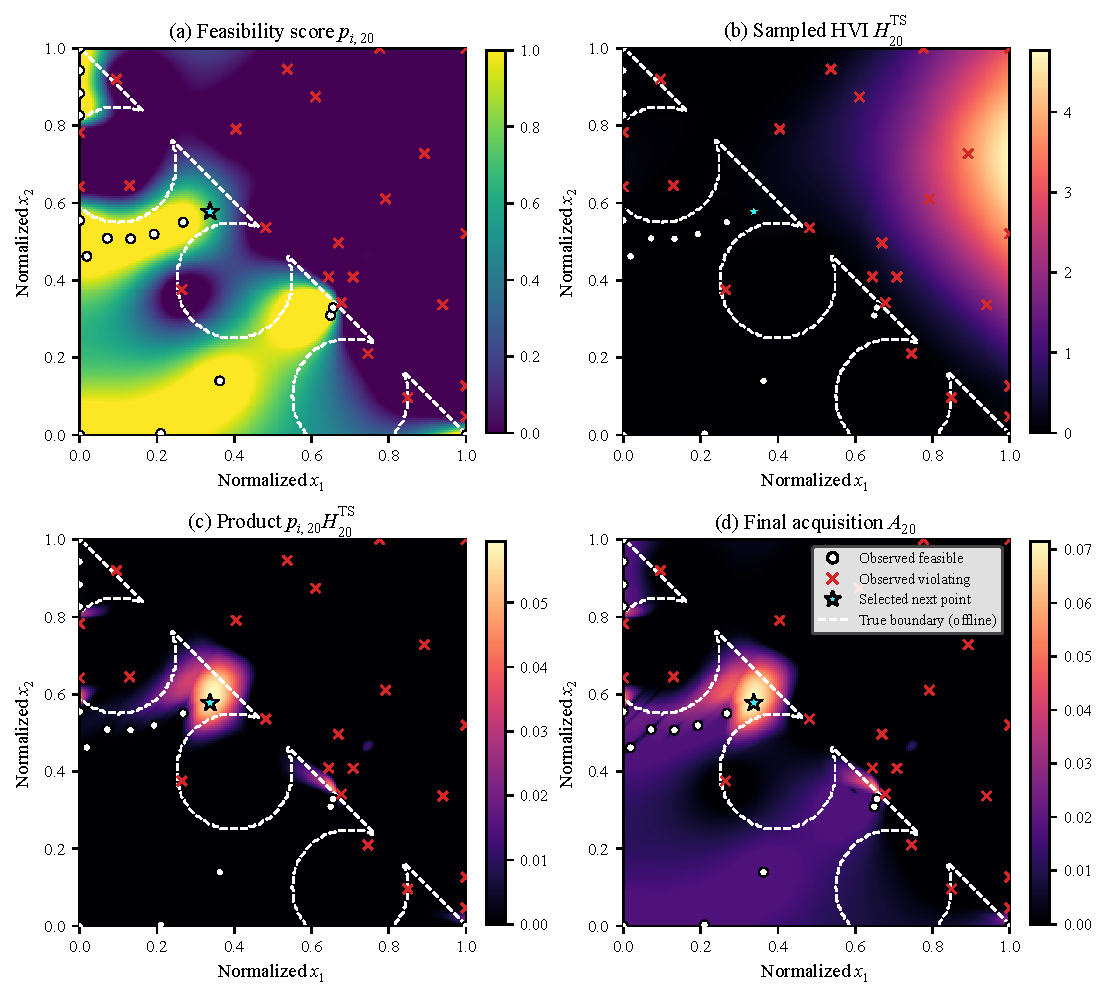
\includegraphics[width=0.99\linewidth]
  {../artifacts/two_dimensional_campaign/figures/cossin2_acquisition_decomposition.pdf}
\caption{COSSIN2 acquisition fields at stored iteration 20: feasibility score,
sampled HVI, their product, and the masked acquisition. \textit{Source:}
Authors' post-processing of the retained run record and analytical COSSIN2
constraints.}
\label{fig:cossin2-acquisition-decomposition}
\end{figure}

\begin{table}[H]
\centering
\caption{Initial and final two-dimensional feasibility-field diagnostics.}
\label{tab:current-2d-pof-metrics}
\footnotesize
\setlength{\tabcolsep}{3.5pt}
\begin{tabular}{@{}llrrrrrrr@{}}
\toprule
Case & Stage & \(N\) & Feasible labels & AUC & Score error &
\shortstack{False-feasible\\rate} & \shortstack{False-infeasible\\rate} &
\shortstack{Balanced\\error}\\
\midrule
COSSIN1 & Initial & 20 & 8  & 0.966 & 0.068 & 0.041 & 0.209 & 0.125\\
         & Final   & 50 & 27 & 0.957 & 0.078 & 0.044 & 0.251 & 0.147\\
COSSIN2 & Initial & 20 & 7  & 0.867 & 0.118 & 0.084 & 0.291 & 0.187\\
         & Final   & 80 & 36 & 0.917 & 0.101 & 0.054 & 0.216 & 0.135\\
BNH      & Initial & 10 & 9  & 0.827 & 0.036 & 0.546 & 0.009 & 0.277\\
         & Final   & 40 & 39 & 0.801 & 0.035 & 0.539 & 0.006 & 0.272\\
SRN      & Initial & 10 & 1  & 0.804 & 0.142 & 0.153 & 0.390 & 0.272\\
         & Final   & 40 & 24 & 0.827 & 0.176 & 0.064 & 0.256 & 0.160\\
\bottomrule
\end{tabular}
\parbox{\linewidth}{\footnotesize\textit{Source:} Authors' calculations from
the run records on the same held-out 40,401-point cell-centered grid. Predicted
feasibility uses \(p_i\geq0.5\). Score error is the mean squared score error across all
probes and is therefore weighted by class prevalence.}
\end{table}

For each milestone in Figures~\ref{fig:current-2d-learning} and
\ref{fig:current-2d-learning-cossin2}, the feasibility-score implementation
was refitted offline using only the labels in the corresponding trajectory
prefix. Coordinates, color limits, observation markers, and diagnostic
contours follow Figure~\ref{fig:current-2d-final-pof}. Because cTSEMO selects
for constrained objective improvement rather than uniform field
reconstruction, these domain-wide diagnostics need not improve monotonically.

\begin{figure}[H]
\centering
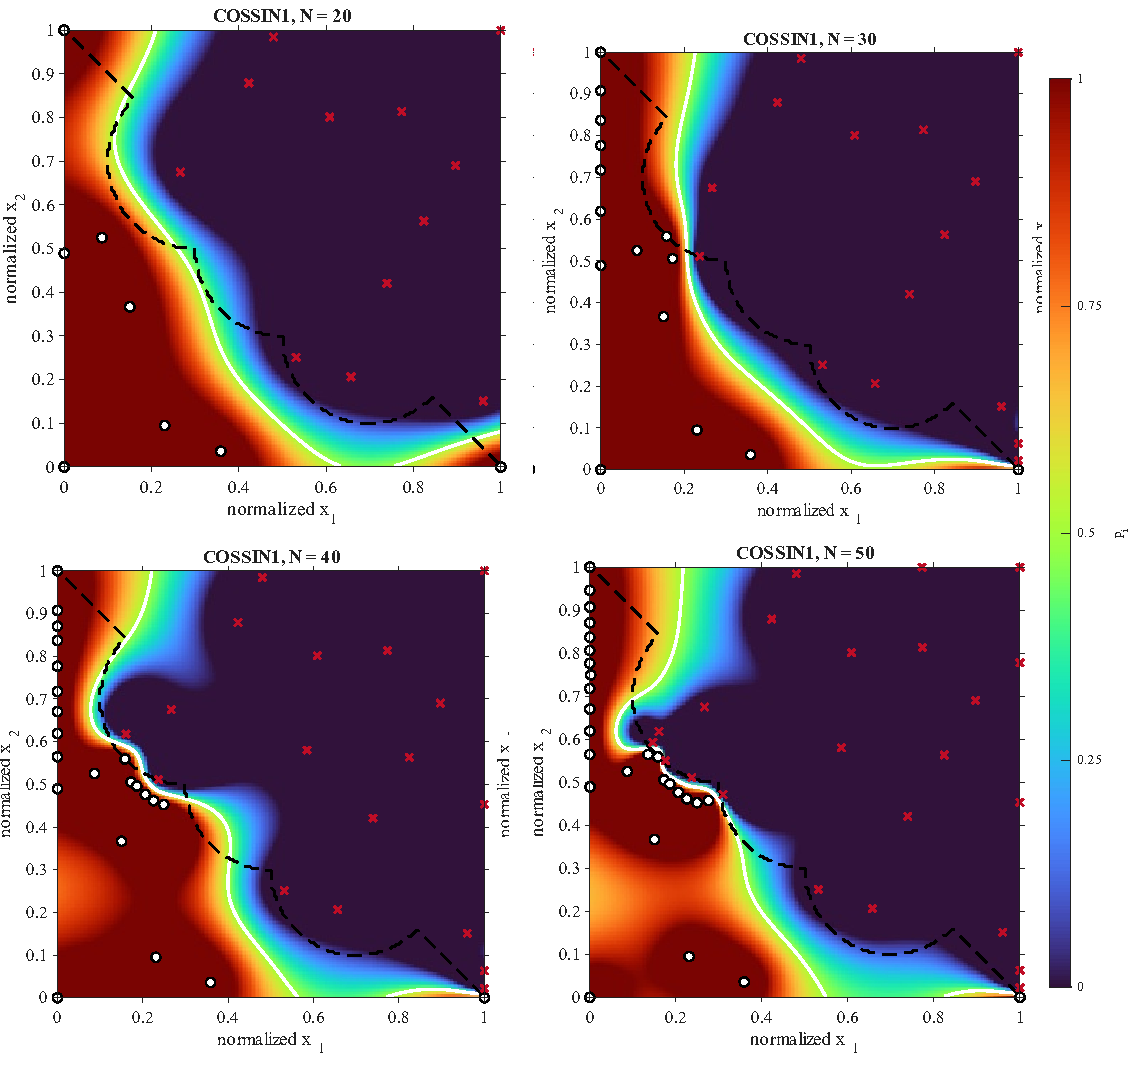
\includegraphics[width=0.90\linewidth]
  {../artifacts/two_dimensional_campaign/figures/cossin1_learning.pdf}
\caption{Offline reconstructions of the clipped \(p_i\) field for COSSIN1
at four stated total-evaluation milestones. \textit{Source:} Authors'
calculations.}
\label{fig:current-2d-learning}
\end{figure}

COSSIN1 did not exhibit uniform field improvement. AUC decreased from 0.966
initially to 0.957 at 50 evaluations, mean squared score error increased from
0.068 to 0.078, and balanced error increased from 0.125 to 0.147. At 40
evaluations, AUC was 0.956 and score error was 0.073, while the initial AUC
remained slightly higher than either later value.

\begin{figure}[H]
\centering
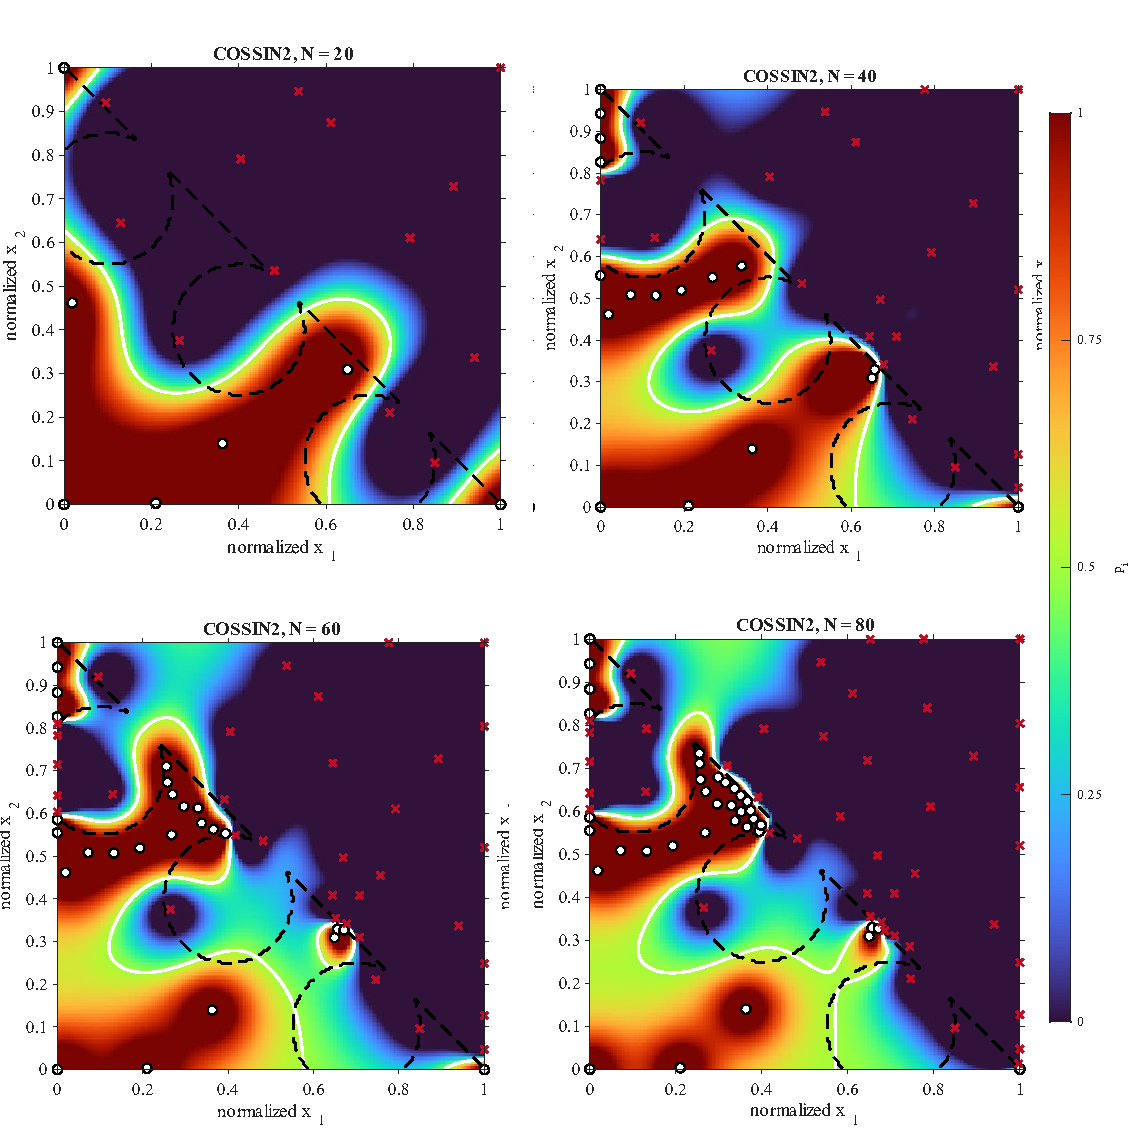
\includegraphics[width=0.90\linewidth]
  {../artifacts/two_dimensional_campaign/figures/cossin2_learning.pdf}
\caption{Offline reconstructions of the clipped \(p_i\) field for COSSIN2
at four stated total-evaluation milestones. \textit{Source:} Authors'
calculations.}
\label{fig:current-2d-learning-cossin2}
\end{figure}

COSSIN2 improved from its initial to final field: AUC increased from 0.867 to
0.917, score error decreased from 0.118 to 0.101, and false-feasible and
false-infeasible rates fell from 0.084 and 0.291 to 0.054 and 0.216,
respectively. The best intermediate field occurred at 40 evaluations, with
AUC 0.940 and score error 0.079, so the improvement was not monotonic.
\FloatBarrier

The two remaining cases expose complementary behavior. The feasible fraction
of the BNH diagnostic grid is 0.936, and 39 of the 40
evaluated designs were feasible.  Its final false-feasible rate within the rare
violating class remained 0.539, while AUC decreased from 0.827 to 0.801.  Thus
its low final mean squared score error of 0.035 is dominated by the prevalent feasible
region and does not imply balanced boundary recovery.  For SRN, both
thresholded error rates and balanced error decreased, the latter from 0.272 to
0.160. AUC also increased from 0.804 to 0.827, whereas the mean squared score error
increased from 0.142 to 0.176.  No single field metric therefore summarizes
all changes in ranking, thresholded geometry, and score magnitude.

Figure~\ref{fig:current-2d-errors} locates the four thresholded outcome classes
on the common diagnostic grid using \(p_i\geq0.5\).

\conditionalfigure[0.99\linewidth]
  {../artifacts/two_dimensional_campaign/figures/classification_error_maps.pdf}
  {Classification outcomes for the four final fields: correctly classified
  feasible, correctly classified violating, false-feasible, and
  false-infeasible probes.}
  {fig:current-2d-errors}
  {Authors' calculations.}
\FloatBarrier

All initial and final fields reproduced the stored labels exactly after
snapping. Clipping also produced substantial point masses: 57.0\% and 48.5\%
of the final COSSIN1 and COSSIN2 probes were zero, while 72.3\% of the BNH
probes were one. The classification maps show where these saturated
predictions agreed or disagreed with benchmark truth.
\FloatBarrier

\section{Fixed-budget higher-dimensional results}
\label{sec:dimension-results}

\subsection{Feasibility-field diagnostics}

All 35 trajectories in the protocol of
Section~\ref{sec:dimension-protocol} completed the prescribed 150 evaluations.
The final fields and run records passed 24 campaign checks covering
benchmark-label construction, snapped-anchor reproduction, prediction bounds,
confusion-count consistency, and record completeness. Each trajectory
comprised 20 initial and 130 sequential evaluations; statistical replication
remained five trajectories per instance. Final threshold metrics used
\(p_i\geq0.5\) on a held-out Latin-hypercube set of 262,144 probes per
problem.

Table~\ref{tab:dimension-absolute} reports median final field metrics. Paired
changes below are medians of the five within-replicate differences.

\begin{table}[H]
\centering
\caption{Median final clipped-GP feasibility-field diagnostics over five runs.}
\label{tab:dimension-absolute}
\footnotesize
\setlength{\tabcolsep}{3.0pt}
\begin{tabular}{@{}lrrrrrrr@{}}
\toprule
Problem & \(d\) & Feasible probes (\%) & AUC &
\shortstack{False-feasible\\rate (\%)} &
\shortstack{False-infeasible\\rate (\%)} &
\shortstack{Balanced\\error (\%)} &
\shortstack{Balanced\\score error}\\
\midrule
Welded-beam variant & 4 & 33.27 & 0.929 & 6.4 & 19.1 & 14.5 & 0.108\\
CF1 & 4 & 49.66 & 0.818 & 7.9 & 58.5 & 33.2 & 0.219\\
CF1 & 10 & 52.40 & 0.651 & 5.2 & 83.5 & 44.5 & 0.336\\
C2-DTLZ2, \(r=0.2\) & 4 & 13.04 & 0.532 & 10.0 & 71.6 & 40.1 & 0.253\\
C2-DTLZ2, \(r=0.2\) & 6 & 2.81 & 0.500 & 0.7 & 91.0 & 45.9 & 0.427\\
MW7 & 4 & 4.37 & 0.448 & 1.5 & 72.3 & 36.6 & 0.316\\
MW7 & 6 & 0.64 & 0.516 & 0.1 & 92.3 & 46.2 & 0.417\\
\bottomrule
\end{tabular}
\parbox{\linewidth}{\footnotesize\textit{Source:} Authors' calculations from
the held-out 262,144-point probe sets. Balanced score error is the mean of the
two class-specific mean squared score errors. The probe fraction is a
diagnostic measure, not the continuous feasible volume. Except for the probe
fraction, columns are medians of per-run metrics; consequently, median balanced
error need not equal one half of the two displayed marginal-median false rates.}
\end{table}

Median AUC was near 0.5 for both C2-DTLZ2 instances and was 0.448 for MW7 at
\(d=4\), indicating weak discrimination on these cases.

For the evaluated clipped Gaussian-process mean, balanced error increased in
13 of the 15 matched higher- versus lower-dimensional replicate pairs. The paired
median increases were 7.99 percentage points for CF1, 7.58 points for
C2-DTLZ2, and 3.06 points for MW7. The increase was driven primarily by the
false-infeasible rate rather than by both error types. Paired median
false-feasible rate changed by \(-2.69\), \(-9.99\), and
\(-1.45\) points, respectively, whereas false-infeasible rate increased by 18.64, 26.65, and
6.46 points. At the prespecified \(p_i\geq0.5\) threshold, the
higher-dimensional fields classified a smaller proportion of truly feasible
probes as feasible. Paired changes in balanced score error
of \(+0.113\), \(+0.179\), and \(+0.082\) provide a consistent
continuous-score diagnostic. The balanced score error is the mean of the two
class-conditional mean squared score errors.

In Figure~\ref{fig:dimension-gp-paired}, thin segments connect the five matched
replicate indices and thick segments connect their medians. Gray diamonds show
the five unpaired welded-beam \(d=4\) runs, with a black horizontal marker for their
median.

\begin{figure}[H]
\centering
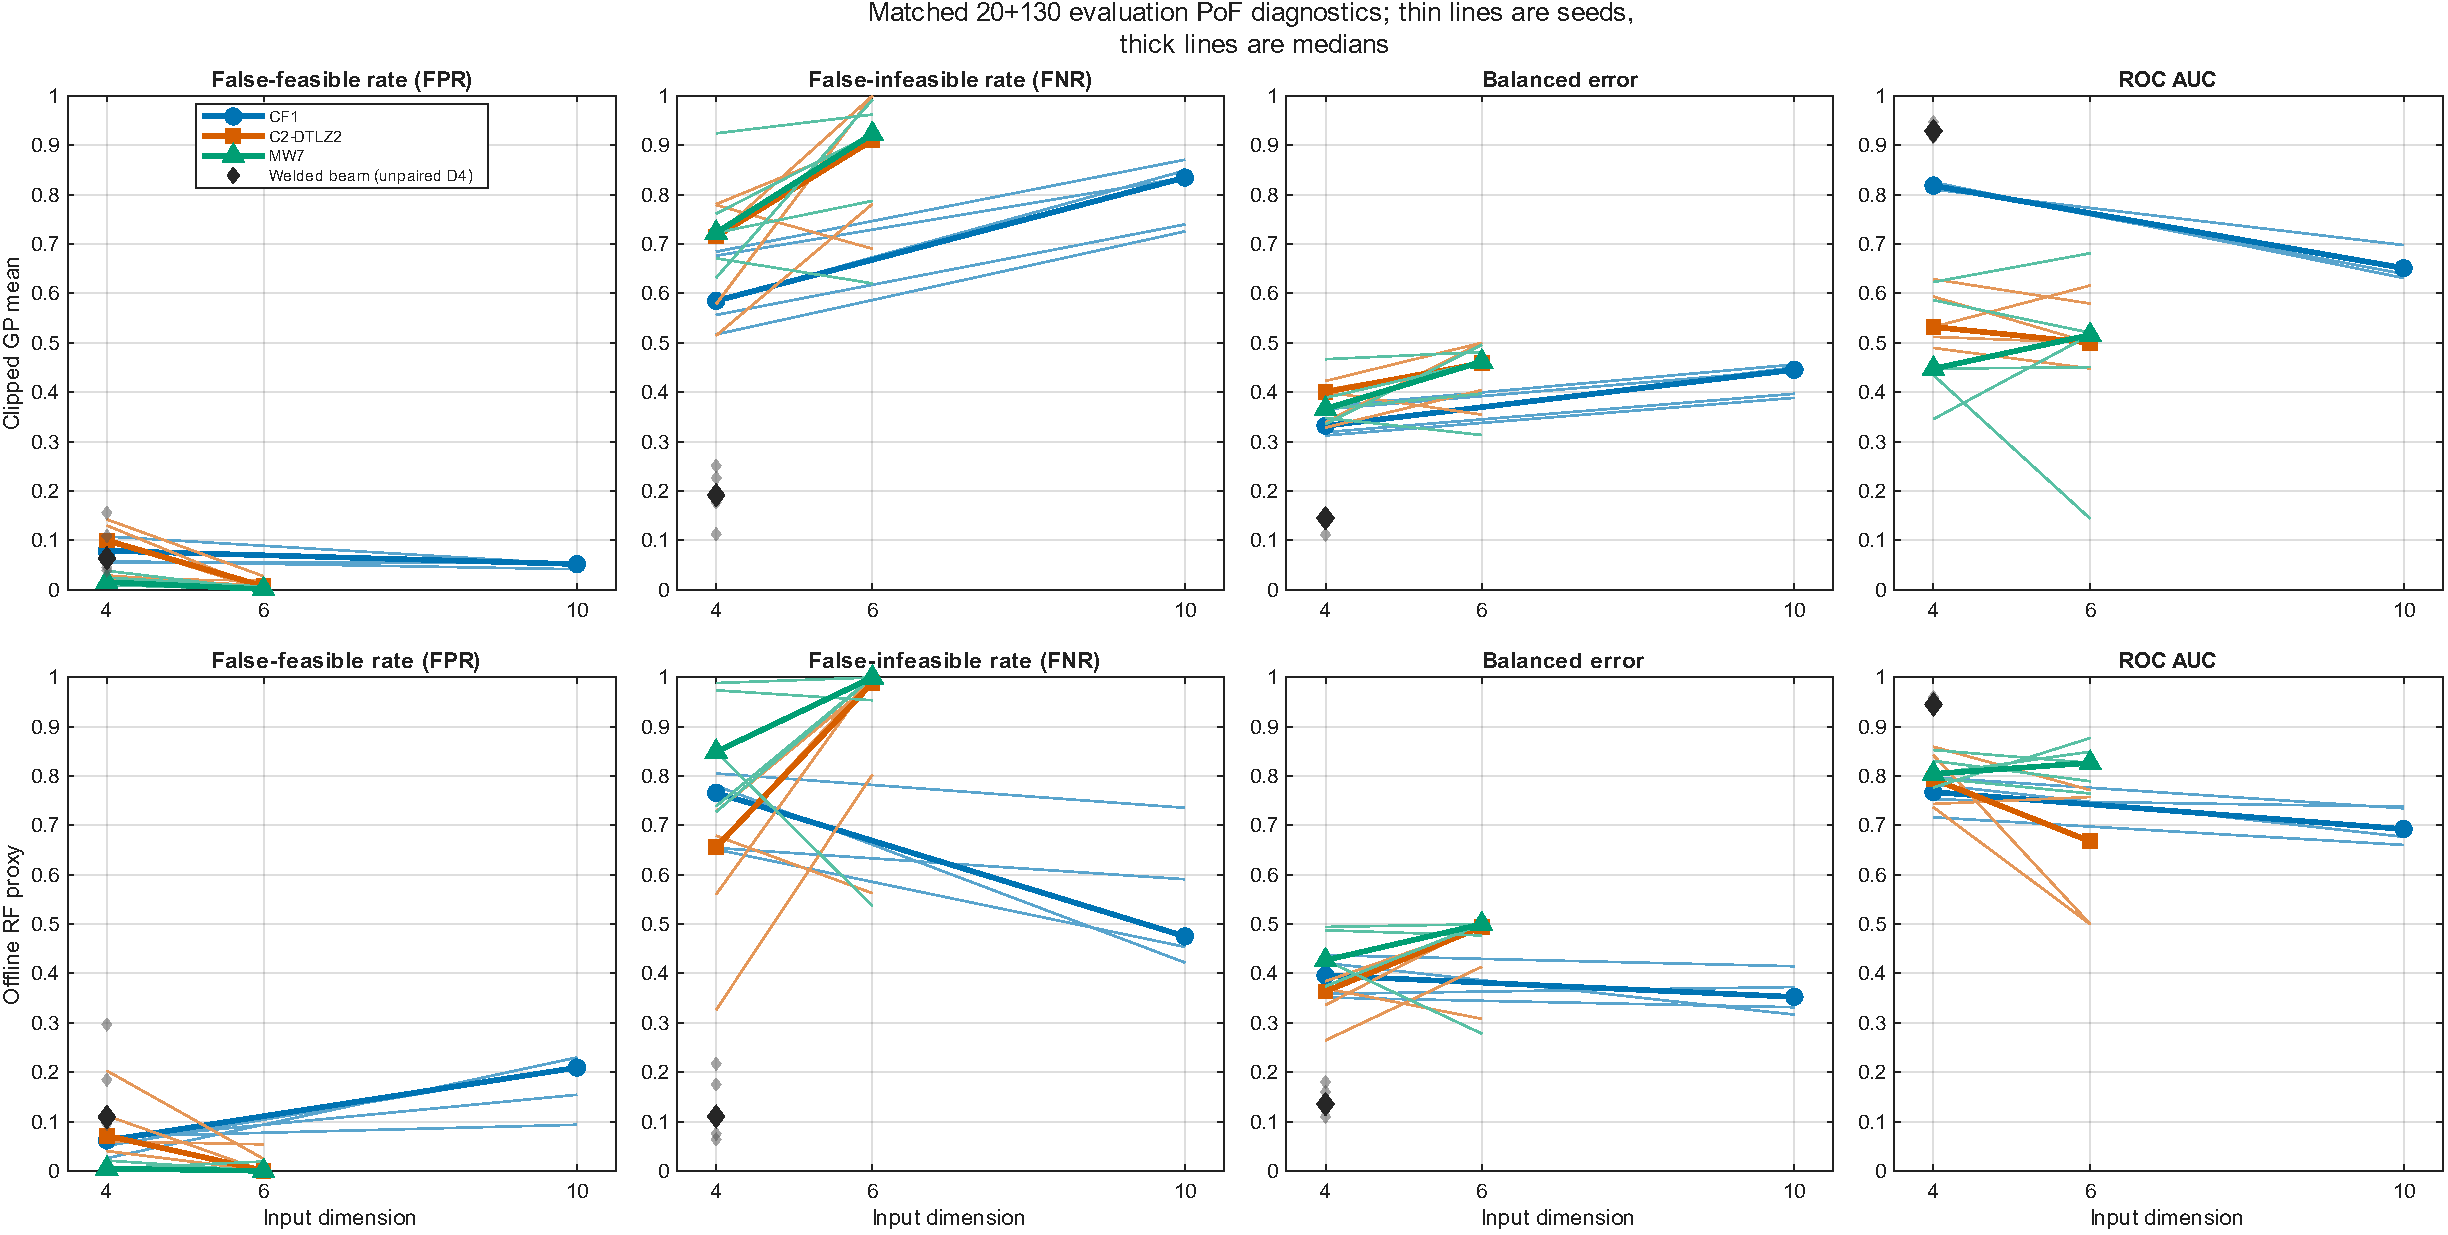
\includegraphics[width=0.98\linewidth,trim={0 296.5bp 587.5bp 35bp},clip]
  {../artifacts/ga_primary_dimension/figures/paired_dimension_gp_rf_metrics.pdf}
\par\vspace{4pt}
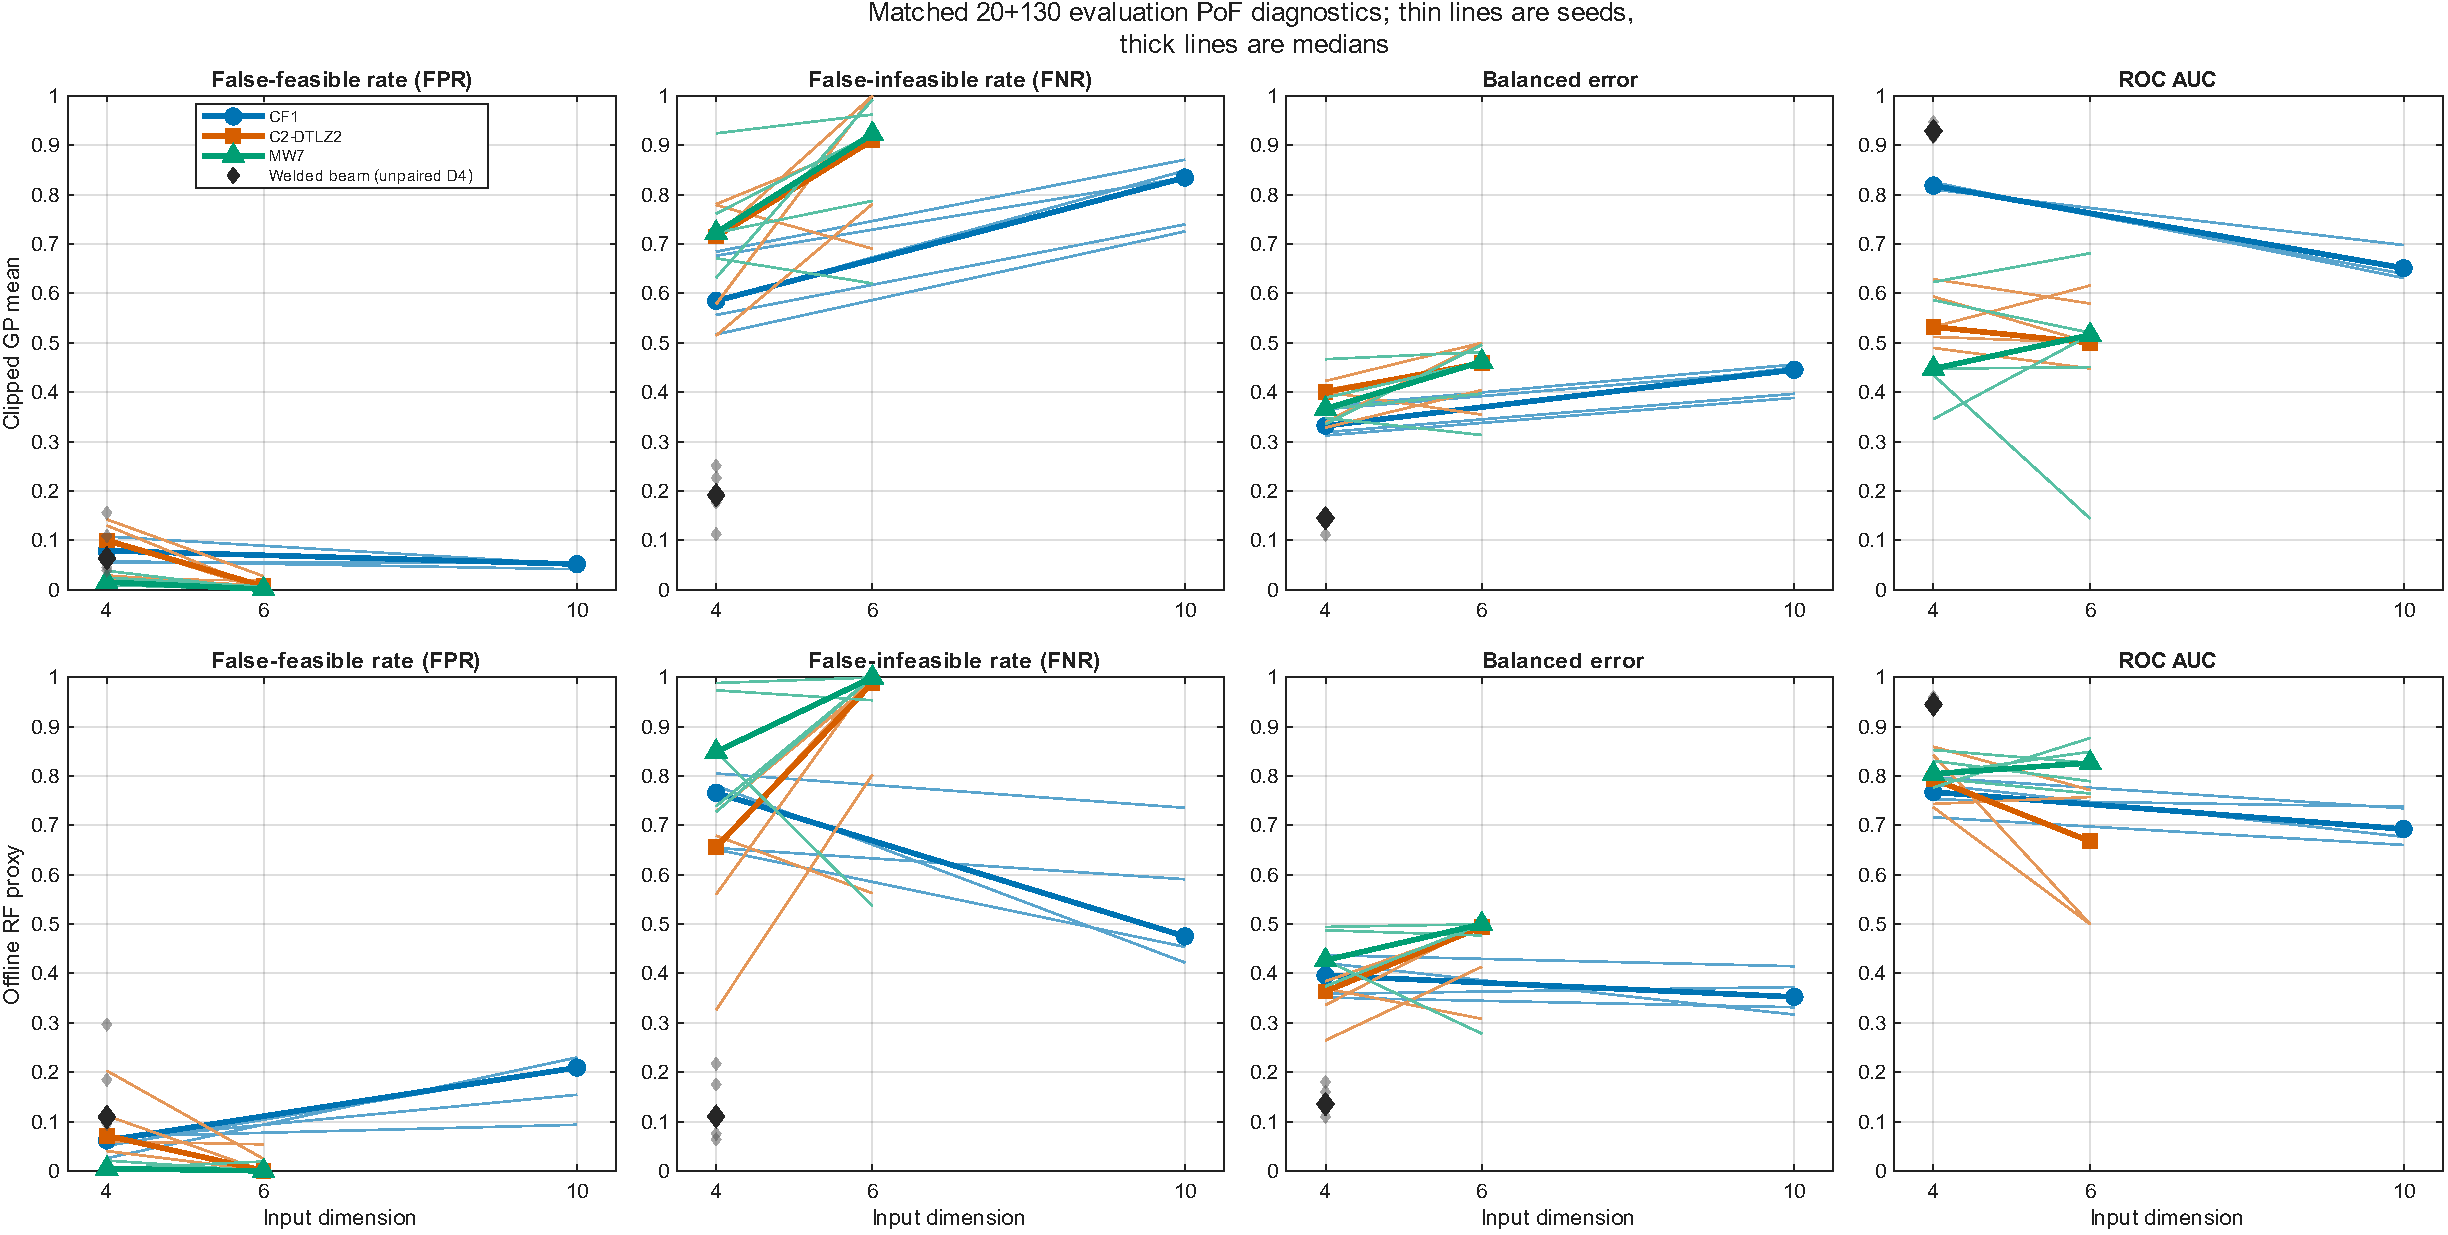
\includegraphics[width=0.98\linewidth,trim={595bp 296.5bp 0 35bp},clip]
  {../artifacts/ga_primary_dimension/figures/paired_dimension_gp_rf_metrics.pdf}
\caption{Paired final diagnostics for the clipped GP-mean field; welded-beam
\(d=4\) results are unpaired references. \textit{Source:} Authors'
calculations.}
\label{fig:dimension-gp-paired}
\end{figure}

CF1 is the least prevalence-confounded dimensional contrast because the
feasible fraction estimated on the held-out probe set remained similar,
changing from 49.66\% at \(d=4\) to 52.40\% at \(d=10\). In contrast, the
estimated feasible fraction changed from 13.04\% to 2.81\% for
C2-DTLZ2 and from 4.37\% to 0.64\% for MW7.  Those two pairs combine
dimension with severe class-prevalence change and are therefore stress-test
evidence rather than causal evidence of a dimension effect.

The offline random-forest (RF) proxy in
Figure~\ref{fig:dimension-rf-paired} demonstrates that the observed
dimensional trend depends on field formulation. Its paired median balanced error decreased by 2.25
points for CF1, while increasing by 13.65 points for C2-DTLZ2 and 0.55
points for MW7. On C2-DTLZ2 at \(d=6\), two of five RF fits predicted no
feasible probe, producing zero false-feasible rate together with unit
false-infeasible rate. Because the RF was fitted to GP-guided trajectories,
these results describe formulation sensitivity.

\begin{figure}[H]
\centering
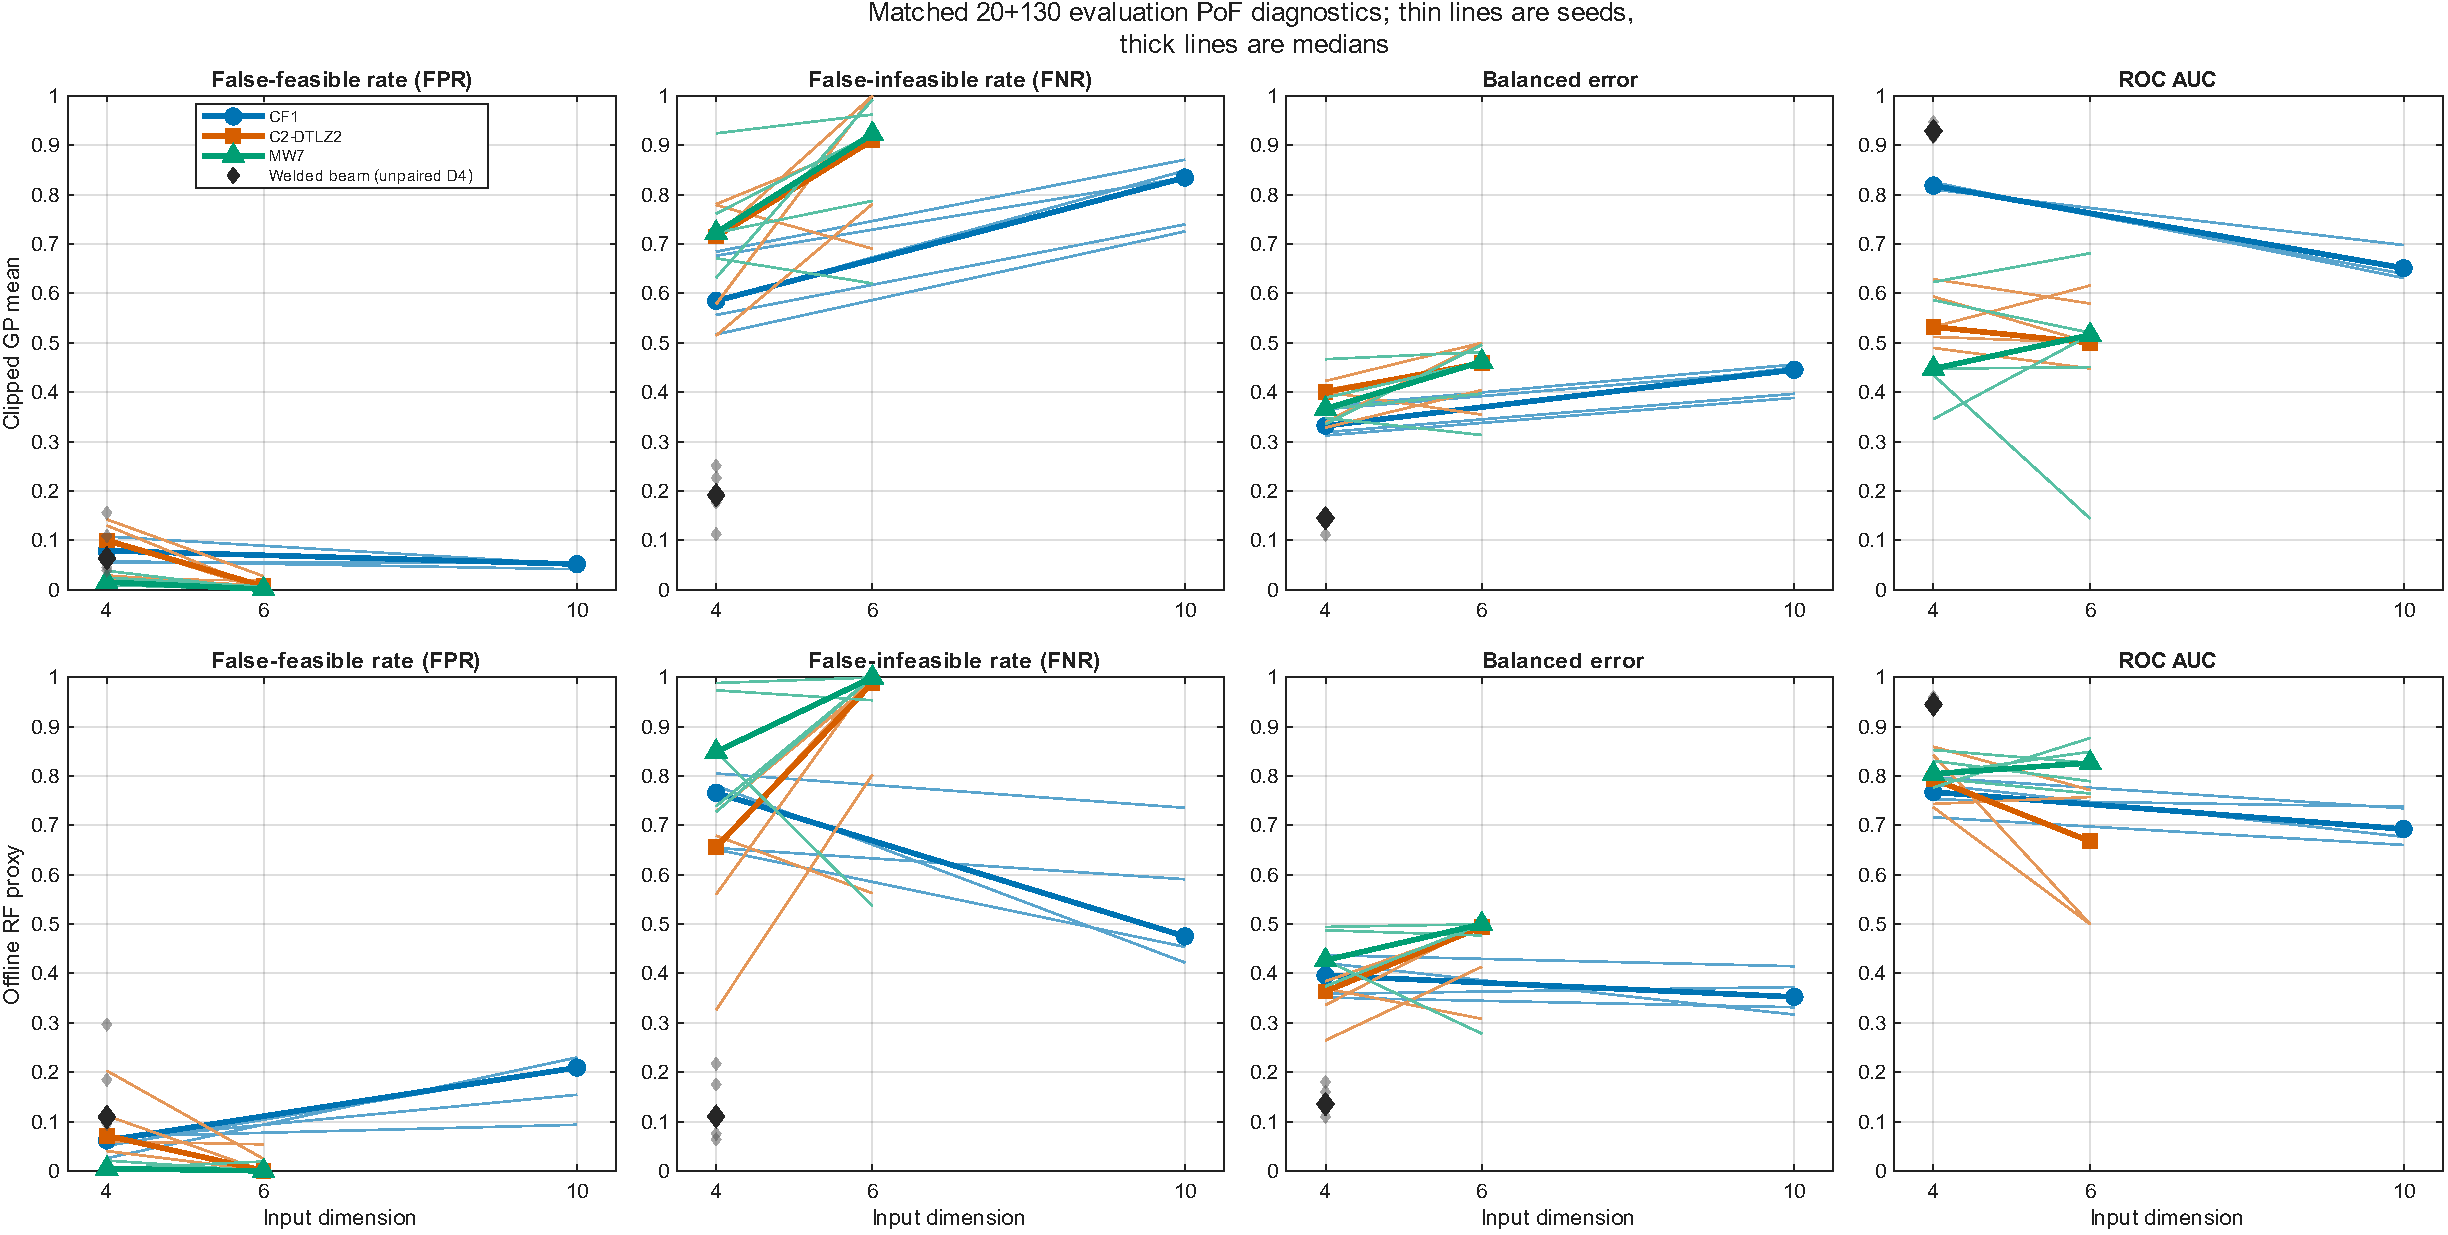
\includegraphics[width=0.98\linewidth,trim={0 0 587.5bp 310bp},clip]
  {../artifacts/ga_primary_dimension/figures/paired_dimension_gp_rf_metrics.pdf}
\par\vspace{4pt}
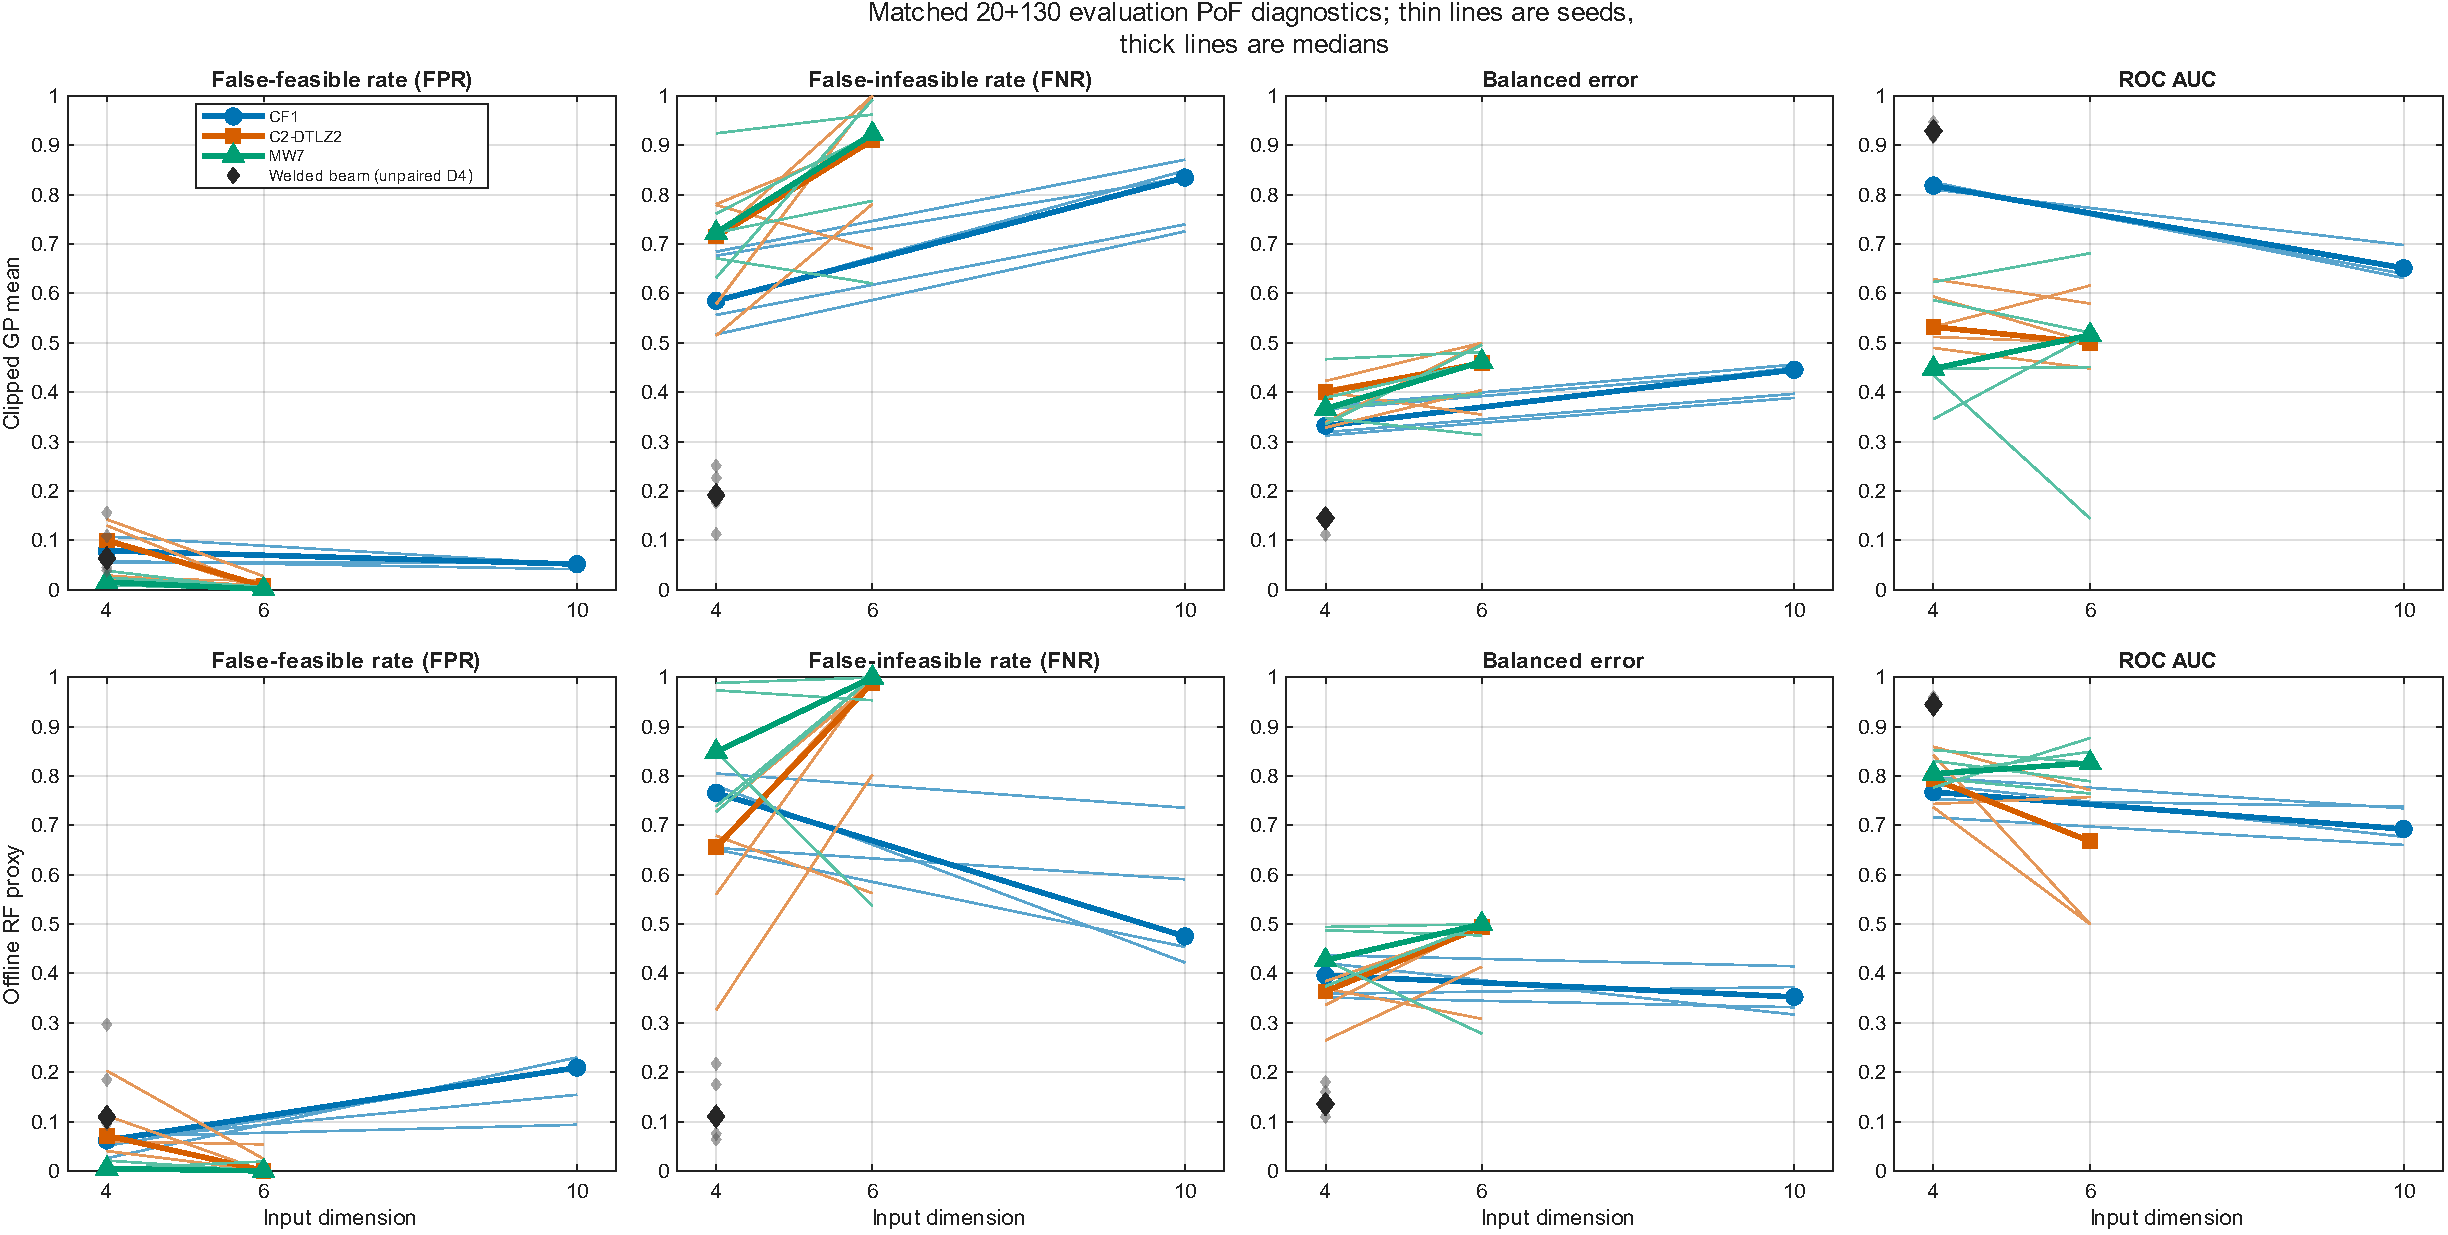
\includegraphics[width=0.98\linewidth,trim={595bp 0 0 310bp},clip]
  {../artifacts/ga_primary_dimension/figures/paired_dimension_gp_rf_metrics.pdf}
\caption{Paired final diagnostics for the offline random-forest proxy fitted
to the GP-guided trajectories. Blue circles, orange squares, green triangles,
and black diamonds denote CF1, C2-DTLZ2, MW7, and the unpaired welded-beam
\(d=4\) runs, respectively. \textit{Source:} Authors' calculations.}
\label{fig:dimension-rf-paired}
\end{figure}

The five-run TSEMO-source welded-beam variant at \(d=4\) had median
GP AUC 0.929, false-feasible rate 6.37\%, false-infeasible rate 19.13\%, and
balanced error 14.49\%. These
values illustrate heterogeneity among four-dimensional cases.

\FloatBarrier
\Needspace{7\baselineskip}
\subsection{Optimization and selection outcomes}
\label{sec:ga-primary-dimension-results}

All 35 GA-primary trajectories completed, comprising 5,250 black-box
evaluations with no failed run. Table~\ref{tab:ga-primary-dimension-results}
summarizes five runs
per instance.  Feasible and nondominated counts are medians with the observed
minimum and maximum in brackets.  A challenger override is counted only among
ordinary primary--challenger decisions; fallback selections use the separate
recovery score.

\begin{table}[H]
\centering
\caption{GA-primary outcomes after 20 initial and 130 sequential
evaluations per run.}
\label{tab:ga-primary-dimension-results}
\footnotesize
\begingroup
\setlength{\tabcolsep}{2.5pt}
\begin{tabular}{@{}l c c c r r r r@{}}
\toprule
Case & \(d\) & Feasible & Nondominated &
\(\widetilde{\mathrm{HV}}_{150}\) & Challenger (\%) &
Fallback (\%) & \(\widetilde t_{\mathrm{acq}}\) (s)\\
\midrule
Welded-beam variant & 4 & 95 [86--109] & 14 [13--16] & 1.2019 & 0.77 & 0.00 & 0.255\\
CF1 & 4 & 40 [27--45] & 11 [9--14] & 1.0849 & 1.85 & 0.00 & 0.232\\
CF1 & 10 & 82 [80--86] & 10 [8--18] & 0.9632 & 0.00 & 0.00 & 0.331\\
C2-DTLZ2, \(r=0.2\) & 4 & 74 [67--79] & 33 [29--39] &
0.5040 & 2.82 & 1.69 & 0.203\\
C2-DTLZ2, \(r=0.2\) & 6 & 9 [0--71] & 1 [0--16] &
0.2620 & 2.56 & 76.00 & 0.030\\
MW7 & 4 & 46 [22--68] & 14 [10--20] & 0.6783 & 3.18 & 8.15 & 0.174\\
MW7 & 6 & 30 [8--65] & 7 [4--13] & 0.4965 & 2.85 & 46.00 & 0.184\\
\bottomrule
\end{tabular}
\endgroup
\parbox{\linewidth}{\footnotesize\textit{Notes:}
\(\widetilde{\mathrm{HV}}_{150}\) is the median final hypervolume in the
normalized objective coordinates defined below; feasible and nondominated
counts are medians with minima and maxima in brackets, and nondominated counts
refer to unique feasible nondominated objective vectors;
\(\widetilde t_{\mathrm{acq}}\) is the median across runs of the mean
per-iteration acquisition time. Challenger and fallback percentages are pooled
across five runs; challenger rates use ordinary primary--challenger decisions
as the denominator, whereas fallback rates use all 650 sequential decisions.
Low \(d=6\) timing values include many
inexpensive fallback iterations. \textit{Source:} Authors' campaign records.}
\end{table}

For the hypervolume histories in
Figure~\ref{fig:ga-primary-dimension-hv}, each problem was assigned one
offline normalization. For objective \(m\), the transformation was
\(\widetilde f_m=(f_m-a_m)/(b_m-a_m)\), where \(a_m\) and \(b_m\) were the
minimum and maximum over the truly feasible held-out probes, as determined by
the benchmark oracle, together with all feasible campaign observations. The
common reference in these coordinates was \((1.1,1.1)\). The rectangle from
the empirical normalization origin \((0,0)\) to this reference has area
\(1.21\). This common post hoc scale enables within-problem comparison of the
five trajectories and removes variation caused by their stored acquisition
references. Values from different problem-specific normalizations are not
comparable across problems. Thin curves denote individual runs, and the black
curve is their pointwise median.

Across the 4,550 sequential decisions, 3,625 selected the GA-primary proposal,
68 selected the independent challenger, and 857 used fallback. Excluding
fallback iterations, the challenger overrode the GA proposal in 68 of 3,693
ordinary decisions (1.84\%); problem-level rates ranged from zero to 3.18\%.
The GA improved on the best of its 1,024 scored reference designs in 3,571 of
those 3,693 eligible iterations (96.7\%). The 1.84\% challenger rate indicates
a limited challenger intervention under this configuration.

Normalized hypervolume increased above its initial-design value in 33 of 35
trajectories. The only zero-growth trajectories were C2-DTLZ2 at \(d=6\),
replicates 2 and 4; both ended without a feasible observation. MW7 at \(d=6\)
found feasible designs in all five runs despite fallback accounting for
46.0\% of sequential decisions. For C2-DTLZ2 at \(d=6\), fallback accounted
for 76.0\% of decisions. These records associate the difficult outcomes with
feasibility-discovery failure and prolonged fallback, while challenger
replacement remained uncommon. Mean acquisition time remained below 0.36~s per iteration for these
analytic benchmarks.

\begin{figure}[!htbp]
\centering
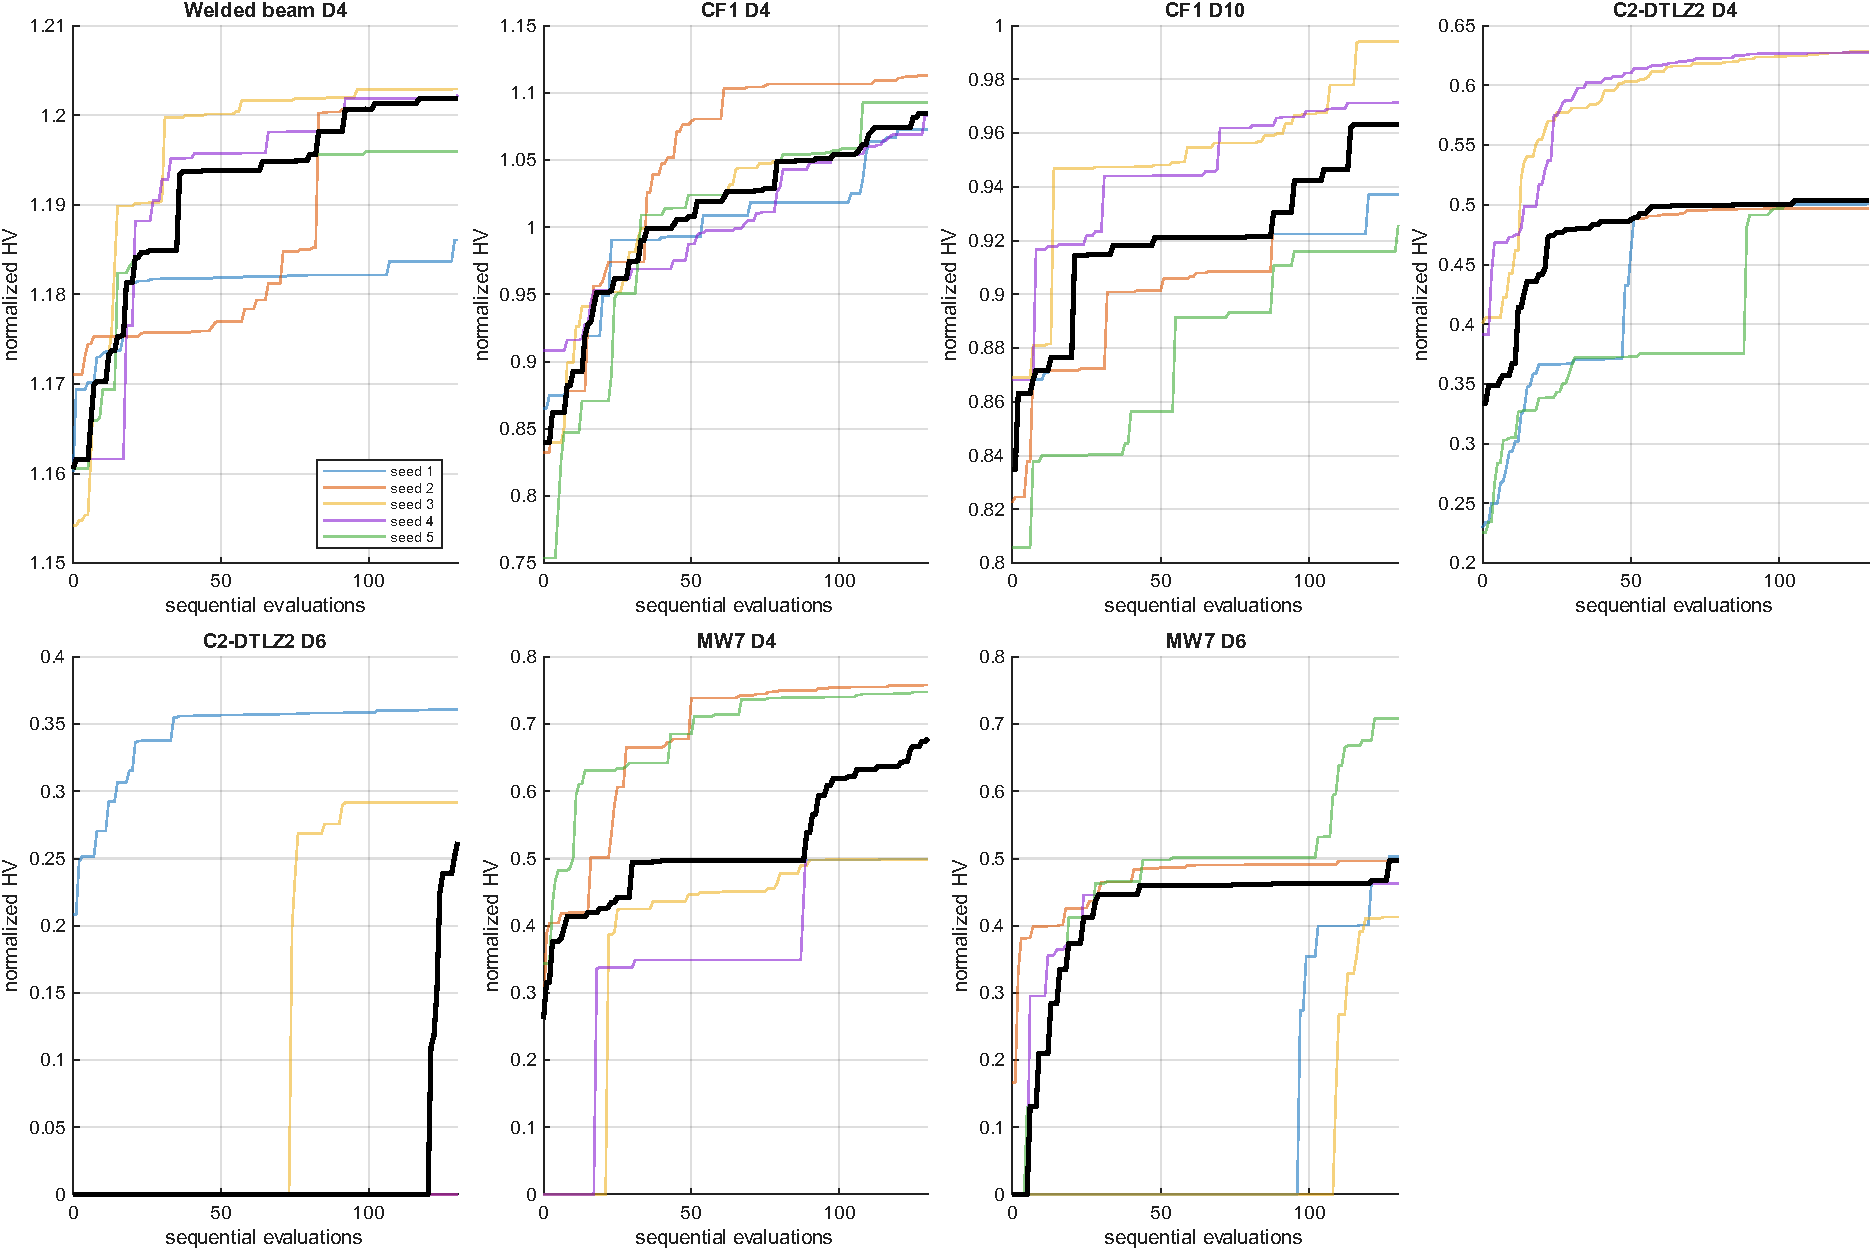
\includegraphics[width=0.99\linewidth,trim={0 300.5bp 450bp 0},clip]
  {../artifacts/ga_primary_dimension/figures/hypervolume_histories.pdf}
\par\vspace{4pt}
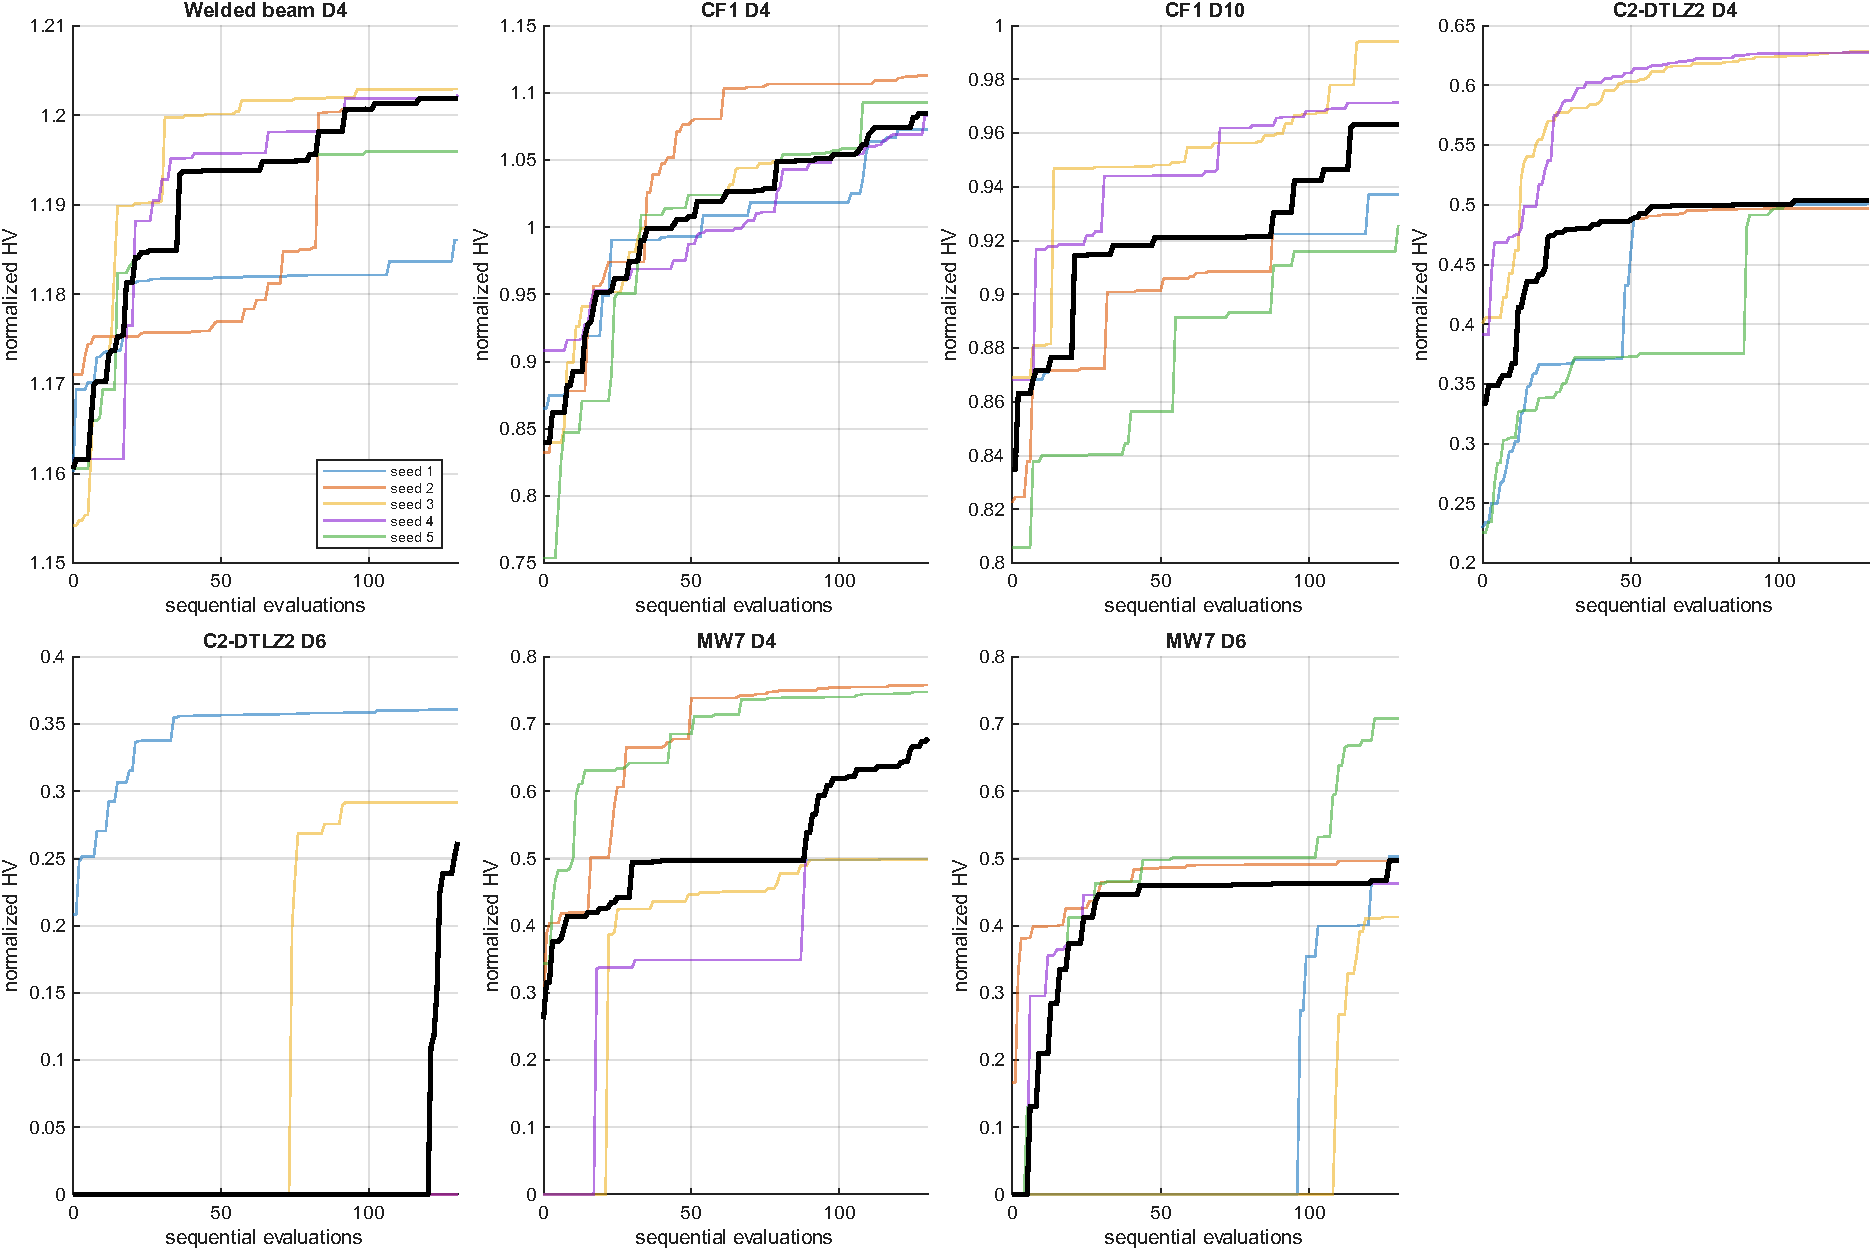
\includegraphics[width=0.99\linewidth,trim={450bp 300.5bp 0 0},clip]
  {../artifacts/ga_primary_dimension/figures/hypervolume_histories.pdf}
\caption{Normalized hypervolume histories for welded-beam, CF1, and
C2-DTLZ2 at \(d=4\); thin curves are individual runs and thick black curves
are pointwise medians. \textit{Source:} Authors' calculations.}
\label{fig:ga-primary-dimension-hv}
\end{figure}

\begin{figure}[!htbp]
\centering
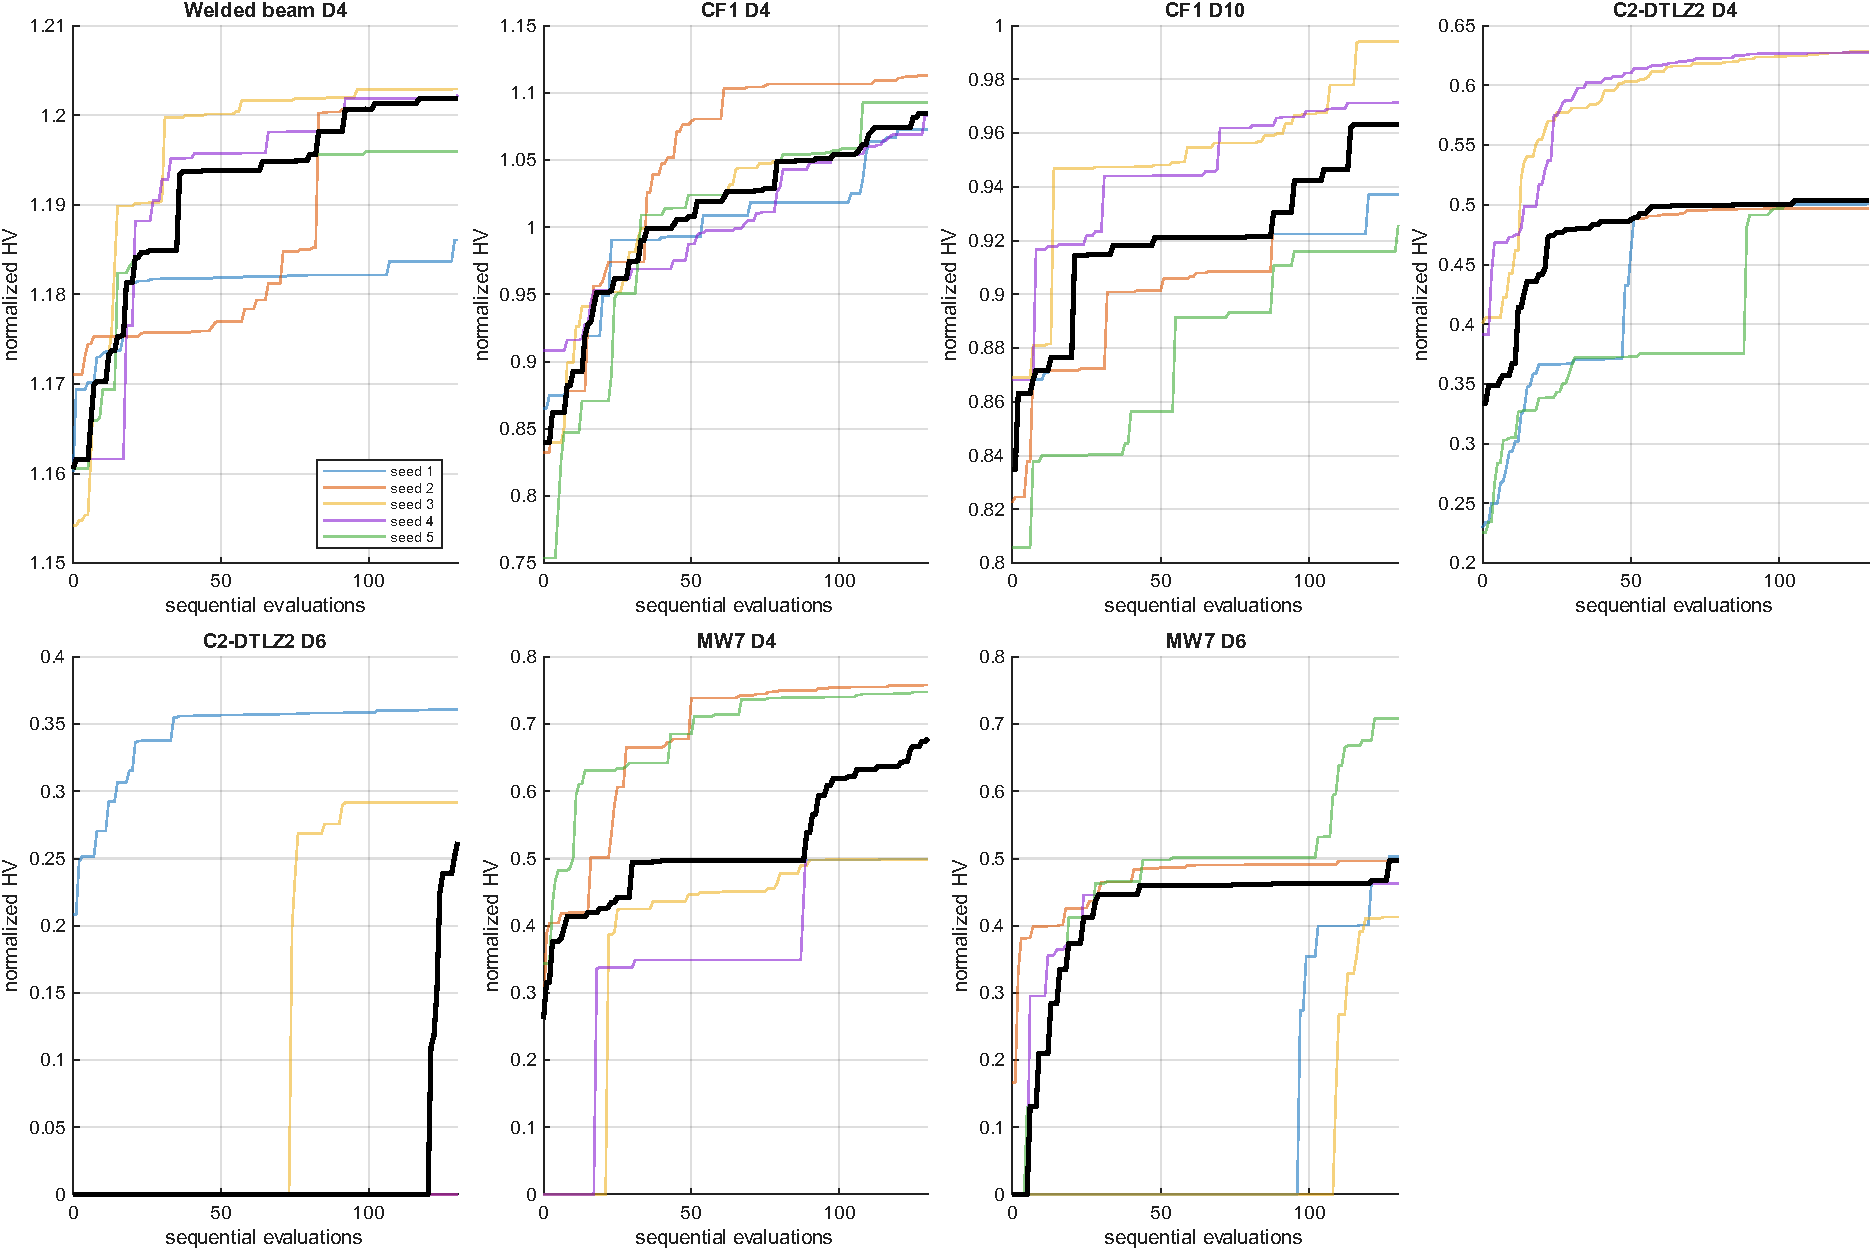
\includegraphics[width=0.99\linewidth,trim={0 0 450bp 300.5bp},clip]
  {../artifacts/ga_primary_dimension/figures/hypervolume_histories.pdf}
\par\vspace{4pt}
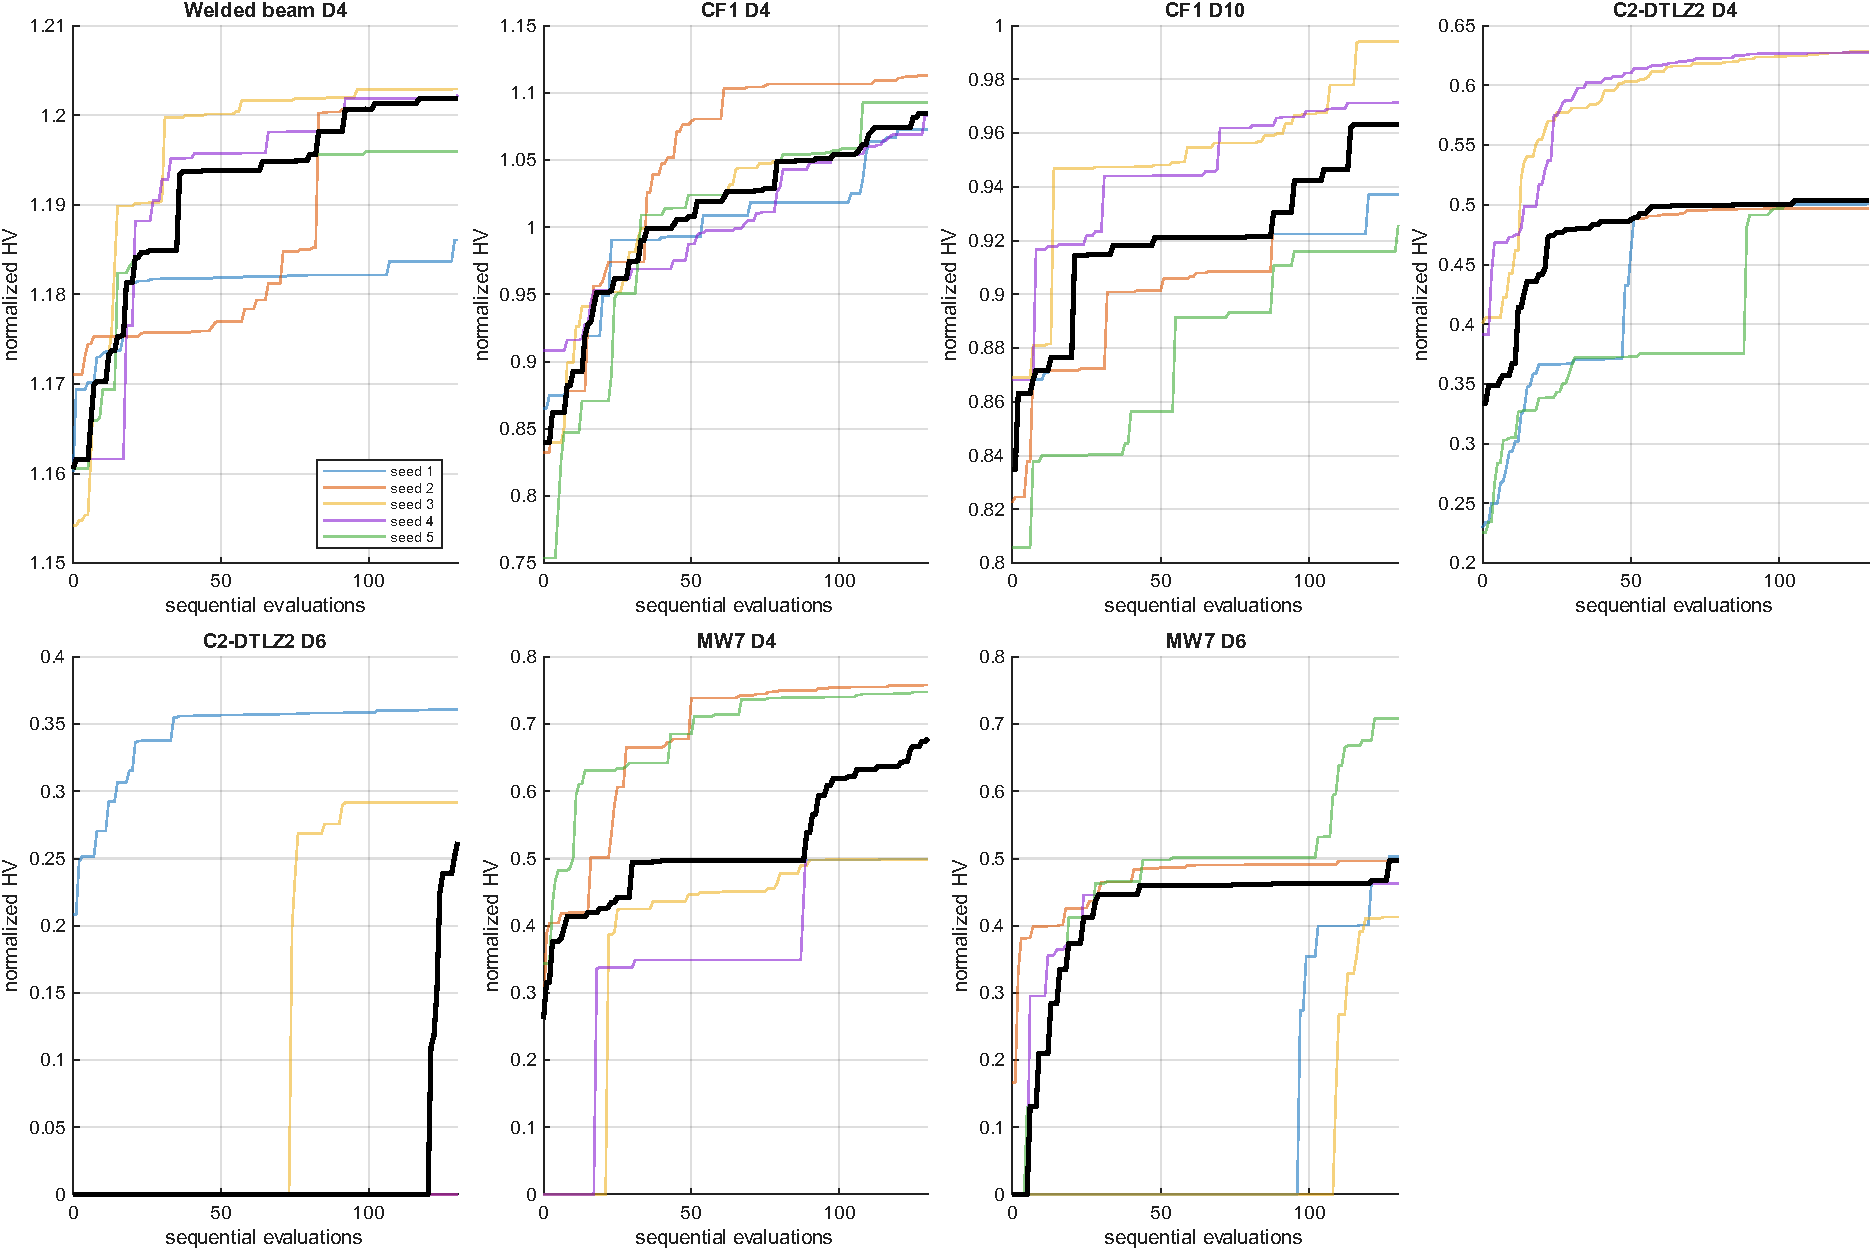
\includegraphics[width=0.49\linewidth,trim={450bp 0 225bp 300.5bp},clip]
  {../artifacts/ga_primary_dimension/figures/hypervolume_histories.pdf}
\caption{Normalized hypervolume histories for C2-DTLZ2 at \(d=6\) and MW7
at \(d=4\) and \(d=6\); thin curves are individual runs and thick black curves
are pointwise medians. \textit{Source:} Authors' calculations.}
\label{fig:ga-primary-dimension-hv-hard}
\end{figure}
\FloatBarrier

\section{Discussion}

\subsection{Clipping, local smoothing, and the anchor convention}

At stored designs, snapping imposes \(p_i=0\) for violating labels and
\(p_i=1\) for feasible labels, while predictions between anchors depend on the
exterior targets, local length field, and clipping. Local enlargement can
suppress oscillatory pockets in densely sampled violating regions but may
erase narrow feasible corridors.

\subsection{Dimension, geometric coverage, and budget interpretation}
\label{sec:dimension-coverage-discussion}

Frazier's low-to-moderate-dimensional regime still permits severe geometric
sparseness under a finite budget, particularly when the same observations must
support two objective models and one aggregate-label feasibility field. For
\(k\) observed designs in the normalized domain, define the
convex-hull fraction as
\[
  V_{\mathrm{hull}}(k,d)=
  \operatorname{Vol}_d\!\left(
  \operatorname{conv}\{\mathbf{u}_1,\ldots,\mathbf{u}_k\}\right).
\]
Because the normalized hypercube has unit volume,
\(V_{\mathrm{hull}}\in[0,1]\). The measure captures global span while counting
the entire hull interior, including unsampled regions; local coverage and
boundary resolution require separate diagnostics.

To frame the largest hull attainable from \(k\) points, let
\[
  M(d,k)=\max_{\mathbf{u}_1,\ldots,\mathbf{u}_k\in[0,1]^d}
  V_{\mathrm{hull}}(k,d).
\]
Only several endpoint cases are required for the present argument. The hull
has zero \(d\)-volume when \(k\leq d\). For \(k=d+1\), an affinely independent
set forms a \(d\)-simplex, and \(M(d,d+1)=D_d/d!\), where \(D_d\) is the
maximum absolute determinant of a \(d\)-by-\(d\) \(0/1\) matrix
\cite{zong2005unitcubes,oeisA003432}. This most favorable simplex fraction
decreases from \(0.125\) at \(d=4\) to \(0.0125\) at \(d=6\),
\(8.82\times10^{-5}\) at \(d=10\), and \(2.33\times10^{-11}\) at \(d=20\).
For intermediate \(d+1<k<2^d\), no general maximum is asserted here.

A complementary construction uses every cube corner except one. It requires
\(2^d-1\) points and encloses the fraction \(1-1/d!\), giving the constructive
bound \(M(d,2^d-1)\geq1-1/d!\). Inverting its point count gives the
vertex-count reference \(d_v(N)=\lfloor\log_2(N+1)\rfloor\). Thus \(N=150\)
gives \(d_v=7\), whereas the corresponding construction requires 1,023 points
in ten dimensions and 1,048,575 points in twenty dimensions. This
all-but-one-corner construction is an optimistic geometric reference. Its
exponential point count illustrates the growth of global coverage
requirements, while \(d_v(N)\) supplies neither a budget prescription nor a
convergence criterion and can leave interior or disconnected feasible regions
unresolved.

Figure~\ref{fig:dimension-hull-coverage} complements these endpoint results
with numerically computed hull growth for successive prefixes of one
fixed-seed, 200-point maximin-Latin-hypercube design per dimension. At
\(k=150\), the observed
hull fractions were \(0.548\), \(0.206\), and \(0.0465\) for \(d=4\), 6, and 8,
respectively. The \(d=9\) and \(d=10\) calculations stopped at 147 and 101
points under the computation safeguard. These curves are illustrative single
design-sequence realizations of geometric coverage.

\begin{figure}[!t]
  \centering
  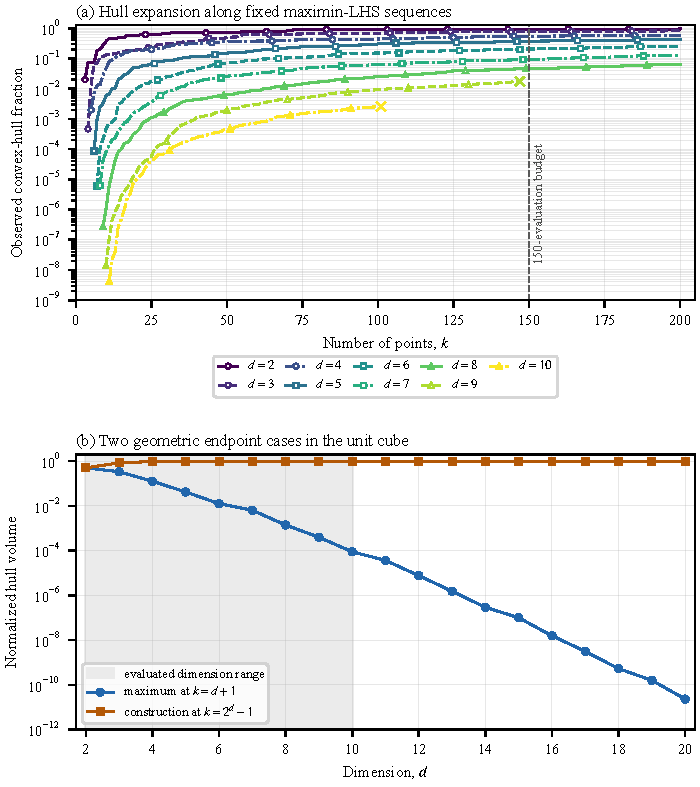
\includegraphics[width=0.98\linewidth]
    {../artifacts/hull_coverage/dimension_hull_coverage.pdf}
  \caption{Convex-hull coverage diagnostics in the normalized hypercube:
  fixed-seed LHS-prefix volumes and two geometric endpoint constructions.
  \textit{Source:} Authors' calculations from the retained deterministic
  designs and OEIS A003432 maximum-determinant data.}
  \label{fig:dimension-hull-coverage}
\end{figure}

cTSEMO evaluates the GP mean throughout the normalized hypercube. Predictions
outside the observed hull are kernel extrapolations governed by the prior
mean, covariance, and labels. Distance-based recovery can enlarge the hull
incidentally, while candidate selection itself remains independent of hull
volume. This retains the possibility of proposing outside the observed hull;
exploration beyond regions favored by the ordinary acquisition depends on the
finite recovery pools.

The matched screen indicates a fixed-budget coverage challenge for the clipped
GP mean. Dimension, boundary geometry, feasible fraction, and the
dimension-dependent local covariance are entangled in the observed changes.
Across the three families, higher-dimensional instances generally had larger
false-infeasible rates and balanced errors, while false-feasible rates did not
increase. The contrasting CF1 random-forest result further shows dependence on
the field formulation. Dimensional reporting should therefore retain both
false rates, balanced error, AUC, feasible prevalence, and the sampling
measure.
\FloatBarrier

\subsection{Role of the feasibility score}

The feasibility score modulates the sampled objective improvement used for
candidate selection. With \(\alpha=1\),
Equation~\eqref{eq:main-acquisition} uses both its ranking and numerical
magnitude. Increasing \(\alpha\) favors higher-score regions but may slow
discovery of disconnected feasible sets. For \(\alpha>0\), clipped-zero
regions receive zero main acquisition, and the recovery policies provide their
alternative route back into the search.

In regions unsupported by observations, a prior-like score expresses limited
information without forcing a confident prediction. The combined field and
recovery policy should be assessed through matched-budget
constrained-selection outcomes.

\subsection{Primary search, challenger, and fallback}

The challenger evaluates the same \(A_k\) as the GA proposal, so an override
indicates that the independent finite LHS set contains a larger evaluated
acquisition value than the finite-budget GA result. It therefore serves as an
acquisition-search coverage check. Fallback uses the distinct recovery score
\(S_{\mathrm{fb},k}\) and is reported separately.

In the five-seed campaign, the challenger supplied 1.84\% of ordinary
selections, whereas fallback supplied 18.84\% of all sequential selections and
was concentrated in the rare-feasible six-dimensional cases. The difficult
C2-DTLZ2 outcomes coincided with feasibility-discovery difficulty and
prolonged recovery rather than frequent challenger replacement.

\section{Limitations}

The evaluated scope covers two objectives, sequential batches of one, bounded
continuous inputs, deterministic aggregate labels, and finite objective values
at every queried design. Extensions to noisy labels, mixed variables, equality
constraints, larger batches, and hidden constraints remain untested.

Aggregation removes information about which constraint was violated and by
how much. The uncalibrated feasibility score nevertheless enters the
acquisition numerically, and clipping can exclude regions from ordinary
selection. Snapping provides stored-label consistency, while the all-feasible
shortcut adopts an optimistic policy until a violation is observed.

The exterior targets and local length-scale rule contain interacting settings
whose transferability across dimensions, boundary geometries, and feasible
fractions has not been established. No universal evaluation budget follows
from dimension alone. Convex-hull volume is used only as an offline geometric
diagnostic; a large hull neither implies dense sampling nor guarantees
accurate feasibility learning.

Dense GP fitting scales cubically with the number of observations. The masks,
GA settings, challenger size, and fallback settings are heuristic. A
finite-budget GA can miss narrow acquisition maxima, while the finite
no-positive-HVI screen can miss a small positive-HVI region.

The dimensional campaign used five replicates per instance. Changes in
feasible prevalence confound the C2-DTLZ2 and MW7 dimension pairs. The
optimizer study additionally used post hoc objective normalization and
included neither component ablations nor an external solver baseline.
Consequently, the experiments characterize the implementation but do not
establish comparative effectiveness. The reported timings concern analytic
benchmark oracles in one MATLAB environment and do not predict end-to-end cost
for simulations or experiments.

\section{Conclusions and future validation}

This study provides a detailed specification and diagnostic evaluation of a
two-objective, TSEMO-derived search architecture for one aggregate binary
feasibility label. Objective Thompson draws and sampled-HVI utility are
retained, while a bounded GA searches the scalar constrained acquisition and
an independent LHS challenger evaluates the same criterion. The feasibility
channel uses an anchor-snapped, clipped GP mean, and explicit discovery and
recovery states define solver behavior when the feasible archive is empty or
finite reference sets provide no usable ordinary acquisition.

The implementation passed 105 of 105 automated tests, and all 35
higher-dimensional trajectories completed their 150-evaluation budgets. The
challenger overrode the GA proposal in 1.84\% of ordinary decisions, whereas
fallback governed 46\% and 76\% of the two rare-feasible six-dimensional
cases. Two of five harder-case trajectories did not discover a feasible
design, and several sparse instances produced near-chance feasibility-score
ranking.

cTSEMO provides defined and recorded behavior in ordinary,
feasibility-discovery, no-positive-HVI, low-acquisition, and duplicate-prone
states. The automated tests exercised the stated execution paths, and the
results identify feasibility-learning and recovery failure modes that guide the
next validation stage. That stage should compare matched aggregate-label baselines, ablate
individual components, fix reporting references in advance, and increase
replication.

\section*{Statements and Declarations}

\paragraph{Data and code availability.}
The source code, reproduction scripts, and supporting run records for the
reported experiments are available in cTSEMO version 0.2.0 at
\href{https://github.com/globaswu/cTSEMO}{the cTSEMO repository}. The release
includes a machine-readable artifact index linking the retained records to the
reported figures and tables.

\paragraph{Use of generative artificial intelligence.}
OpenAI Codex was used to assist method and implementation development,
source-code inspection and generation, test design, benchmark orchestration,
numerical analysis, figure preparation, literature searches and reference
checking, language editing, and manuscript drafting. The authors made all final
scientific decisions and take responsibility for the final work.

% Author-supplied funding, competing-interests, acknowledgements, and author-
% contribution statements must be inserted here before journal submission.

\small
\begin{thebibliography}{99}

\bibitem{jones1998ego}
D. R. Jones, M. Schonlau, and W. J. Welch.
Efficient global optimization of expensive black-box functions.
\emph{Journal of Global Optimization}, 13(4):455--492, 1998.
\url{https://doi.org/10.1023/A:1008306431147}

\bibitem{forrester2008engineering}
A. I. J. Forrester, A. S\'obester, and A. J. Keane.
\emph{Engineering Design via Surrogate Modelling: A Practical Guide}.
John Wiley \& Sons, Ltd., 2008.
\url{https://doi.org/10.1002/9780470770801}

\bibitem{frazier2018tutorial}
P. I. Frazier.
Bayesian optimization.
In \emph{Recent Advances in Optimization and Modeling of Contemporary
Problems}, INFORMS Tutorials in Operations Research, pp. 255--278, 2018.
\url{https://doi.org/10.1287/educ.2018.0188}

\bibitem{shahriari2016review}
B. Shahriari, K. Swersky, Z. Wang, R. P. Adams, and N. de Freitas.
Taking the human out of the loop: A review of Bayesian optimization.
\emph{Proceedings of the IEEE}, 104(1):148--175, 2016.
\url{https://doi.org/10.1109/JPROC.2015.2494218}

\bibitem{snoek2012practical}
J. Snoek, H. Larochelle, and R. P. Adams.
Practical Bayesian optimization of machine learning algorithms.
\emph{Advances in Neural Information Processing Systems}, 25:2951--2959, 2012.
\url{https://proceedings.neurips.cc/paper_files/paper/2012/hash/05311655a15b75fab86956663e1819cd-Abstract.html}

\bibitem{rasmussen2006gpml}
C. E. Rasmussen and C. K. I. Williams.
\emph{Gaussian Processes for Machine Learning}. MIT Press, 2006.
\url{https://doi.org/10.7551/mitpress/3206.001.0001}

\bibitem{gardner2014constraints}
J. R. Gardner, M. J. Kusner, Z. E. Xu, K. Q. Weinberger, and J. Cunningham.
Bayesian optimization with inequality constraints.
\emph{Proceedings of the 31st International Conference on Machine Learning},
PMLR 32(2):937--945, 2014.
\url{https://proceedings.mlr.press/v32/gardner14.html}

\bibitem{gelbart2014unknown}
M. A. Gelbart, J. Snoek, and R. P. Adams.
Bayesian optimization with unknown constraints.
\emph{Proceedings of the Thirtieth Conference on Uncertainty in Artificial
Intelligence}, pp. 250--259, AUAI Press, 2014.
\url{https://auai.org/uai2014/proceedings/individuals/107.pdf}

\bibitem{emmerich2011ehvi}
M. T. M. Emmerich, A. H. Deutz, and J. W. Klinkenberg.
Hypervolume-based expected improvement: monotonicity properties and exact
computation.
\emph{2011 IEEE Congress of Evolutionary Computation}, pp. 2147--2154, 2011.
\url{https://doi.org/10.1109/CEC.2011.5949880}

\bibitem{daulton2020qehvi}
S. Daulton, M. Balandat, and E. Bakshy.
Differentiable expected hypervolume improvement for parallel multi-objective
Bayesian optimization.
\emph{Advances in Neural Information Processing Systems}, 33:9851--9864, 2020.
\url{https://proceedings.neurips.cc/paper/2020/hash/6fec24eac8f18ed793f5eaad3dd7977c-Abstract.html}

\bibitem{deb2002nsga2}
K. Deb, A. Pratap, S. Agarwal, and T. Meyarivan.
A fast and elitist multiobjective genetic algorithm: NSGA-II.
\emph{IEEE Transactions on Evolutionary Computation}, 6(2):182--197, 2002.
\url{https://doi.org/10.1109/4235.996017}

\bibitem{bradford2018tsemo}
E. Bradford, A. M. Schweidtmann, and A. Lapkin.
Efficient multiobjective optimization employing Gaussian processes,
spectral sampling and a genetic algorithm.
\emph{Journal of Global Optimization}, 71(2):407--438, 2018.
\url{https://doi.org/10.1007/s10898-018-0609-2}

\bibitem{helmdach2017lca}
D. Helmdach, P. Yaseneva, P. K. Heer, A. M. Schweidtmann, and A. A. Lapkin.
A multiobjective optimization including results of life cycle assessment in
developing biorenewables-based processes.
\emph{ChemSusChem}, 10(18):3632--3643, 2017.
\url{https://doi.org/10.1002/cssc.201700927}

\bibitem{schweidtmann2018flow}
A. M. Schweidtmann, A. D. Clayton, N. Holmes, E. Bradford, R. A. Bourne, and
A. A. Lapkin.
Machine learning meets continuous flow chemistry: automated optimization
towards the Pareto front of multiple objectives.
\emph{Chemical Engineering Journal}, 352:277--282, 2018.
\url{https://doi.org/10.1016/j.cej.2018.07.031}

\bibitem{amar2019solvent}
Y. Amar, A. M. Schweidtmann, P. Deutsch, L. Cao, and A. Lapkin.
Machine learning and molecular descriptors enable rational solvent selection
in asymmetric catalysis.
\emph{Chemical Science}, 10(27):6697--6706, 2019.
\url{https://doi.org/10.1039/C9SC01844A}

\bibitem{clayton2020selfoptimisation}
A. D. Clayton, A. M. Schweidtmann, G. Clemens, J. A. Manson, C. J. Taylor,
C. G. Ni\~no, T. W. Chamberlain, N. Kapur, A. J. Blacker, A. A. Lapkin, and
R. A. Bourne.
Automated self-optimisation of multi-step reaction and separation processes
using machine learning.
\emph{Chemical Engineering Journal}, 384:123340, 2020.
\url{https://doi.org/10.1016/j.cej.2019.123340}

\bibitem{bachoc2020failures}
F. Bachoc, C. Helbert, and V. Picheny.
Gaussian process optimization with failures: classification and convergence
proof.
\emph{Journal of Global Optimization}, 78(3):483--506, 2020.
\url{https://doi.org/10.1007/s10898-020-00920-0}

\bibitem{candelieri2021partially}
A. Candelieri.
Sequential model based optimization of partially defined functions under
unknown constraints.
\emph{Journal of Global Optimization}, 79(2):281--303, 2021.
\url{https://doi.org/10.1007/s10898-019-00860-4}

\bibitem{letham2019noisy}
B. Letham, B. Karrer, G. Ottoni, and E. Bakshy.
Constrained Bayesian optimization with noisy experiments.
\emph{Bayesian Analysis}, 14(2):495--519, 2019.
\url{https://doi.org/10.1214/18-BA1110}

\bibitem{platt1999probabilistic}
J. C. Platt.
Probabilistic outputs for support vector machines and comparisons to
regularized likelihood methods.
In A. J. Smola, P. L. Bartlett, B. Sch\"olkopf, and D. Schuurmans, editors,
\emph{Advances in Large Margin Classifiers}, pp. 61--74, MIT Press, 1999.

\bibitem{basudhar2012svm}
A. Basudhar, C. Dribusch, S. Lacaze, and S. Missoum.
Constrained efficient global optimization with support vector machines.
\emph{Structural and Multidisciplinary Optimization}, 46(2):201--221, 2012.
\url{https://doi.org/10.1007/s00158-011-0745-5}

\bibitem{lee2011hidden}
H. K. H. Lee, R. B. Gramacy, C. Linkletter, and G. A. Gray.
Optimization subject to hidden constraints via statistical emulation.
\emph{Pacific Journal of Optimization}, 7(3):467--478, 2011.
\url{http://www.ybook.co.jp/online2/oppjo/vol7/p467.html}

\bibitem{nardi2019hypermapper}
L. Nardi, D. Koeplinger, and K. Olukotun.
Practical design space exploration.
\emph{2019 IEEE 27th International Symposium on Modeling, Analysis, and
Simulation of Computer and Telecommunication Systems (MASCOTS)},
pp. 347--358, 2019.
\url{https://doi.org/10.1109/MASCOTS.2019.00045}

\bibitem{audet2020binary}
C. Audet, G. Caporossi, and S. Jacquet.
Binary, unrelaxable and hidden constraints in blackbox optimization.
\emph{Operations Research Letters}, 48(4):467--471, 2020.
\url{https://doi.org/10.1016/j.orl.2020.05.011}

\bibitem{tian2024boundary}
Y. Tian, A. Zuniga, X. Zhang, J. P. D\"urholt, P. Das, J. Chen,
W. Matusik, and M. Konakovi\'c Lukovi\'c.
Boundary exploration for Bayesian optimization with unknown physical
constraints.
\emph{Proceedings of the 41st International Conference on Machine Learning},
PMLR 235:48295--48320, 2024.
\url{https://proceedings.mlr.press/v235/tian24g.html}

\bibitem{heese2021binary}
R. Heese and M. Bortz.
Adaptive sampling of Pareto frontiers with binary constraints using
regression and classification.
\emph{2020 25th International Conference on Pattern Recognition (ICPR)},
pp. 3404--3411, 2021.
\url{https://doi.org/10.1109/ICPR48806.2021.9412217}

\bibitem{sattari2024physics}
K. Sattari, Y. Wu, Z. Chen, A. Mahjoubnia, C. Su, and J. Lin.
Physics-constrained multi-objective Bayesian optimization to accelerate
3D printing of thermoplastics.
\emph{Additive Manufacturing}, 86:104204, 2024.
\url{https://doi.org/10.1016/j.addma.2024.104204}

\bibitem{khatamsaz2022materials}
D. Khatamsaz, B. Vela, P. Singh, D. D. Johnson, D. Allaire, and
R. Arr\'oyave.
Multi-objective materials Bayesian optimization with active learning of
design constraints: design of ductile refractory multi-principal-element
alloys.
\emph{Acta Materialia}, 236:118133, 2022.
\url{https://doi.org/10.1016/j.actamat.2022.118133}

\bibitem{khatamsaz2023entropy}
D. Khatamsaz, B. Vela, P. Singh, D. D. Johnson, D. Allaire, and
R. Arr\'oyave.
Bayesian optimization with active learning of design constraints using an
entropy-based approach.
\emph{npj Computational Materials}, 9:49, 2023.
\url{https://doi.org/10.1038/s41524-023-01006-7}

\bibitem{feliot2017constrained}
P. Feliot, J. Bect, and E. Vazquez.
A Bayesian approach to constrained single- and multi-objective optimization.
\emph{Journal of Global Optimization}, 67(1--2):97--133, 2017.
\url{https://doi.org/10.1007/s10898-016-0427-3}

\bibitem{gonzalez2016localpenalization}
J. Gonz\'alez, Z. Dai, P. Hennig, and N. Lawrence.
Batch Bayesian optimization via local penalization.
\emph{Proceedings of the 19th International Conference on Artificial
Intelligence and Statistics}, PMLR 51:648--657, 2016.
\url{https://proceedings.mlr.press/v51/gonzalez16a.html}

\bibitem{morris1995exploratory}
M. D. Morris and T. J. Mitchell.
Exploratory designs for computational experiments.
\emph{Journal of Statistical Planning and Inference}, 43(3):381--402, 1995.
\url{https://doi.org/10.1016/0378-3758(94)00035-T}

\bibitem{paciorek2004nonstationary}
C. J. Paciorek and M. J. Schervish.
Nonstationary covariance functions for Gaussian process regression.
In \emph{Advances in Neural Information Processing Systems 16: Proceedings
of the 2003 Conference}, pp. 273--280, MIT Press, 2004.
\url{https://proceedings.neurips.cc/paper/2003/hash/326a8c055c0d04f5b06544665d8bb3ea-Abstract.html}

\bibitem{wilson2020pathwise}
J. Wilson, V. Borovitskiy, A. Terenin, P. Mostowsky, and M. Deisenroth.
Efficiently sampling functions from Gaussian process posteriors.
\emph{Proceedings of the 37th International Conference on Machine Learning},
PMLR 119:10292--10302, 2020.
\url{https://proceedings.mlr.press/v119/wilson20a.html}

\bibitem{wendland1995compact}
H. Wendland.
Piecewise polynomial, positive definite and compactly supported radial
functions of minimal degree.
\emph{Advances in Computational Mathematics}, 4:389--396, 1995.
\url{https://doi.org/10.1007/BF02123482}

\bibitem{binh1997mobes}
T. T. Binh and U. Korn.
MOBES: A multiobjective evolution strategy for constrained optimization
problems.
In \emph{Proceedings of the Third International Conference on Genetic
Algorithms (Mendel 97)}, Brno, Czech Republic, pp. 176--182, 1997.

\bibitem{deb2005dtlz}
K. Deb, L. Thiele, M. Laumanns, and E. Zitzler.
Scalable test problems for evolutionary multiobjective optimization.
In A. Abraham, L. Jain, and R. Goldberg, editors,
\emph{Evolutionary Multiobjective Optimization: Theoretical Advances and
Applications}, pp. 105--145, Springer, 2005.
\url{https://doi.org/10.1007/1-84628-137-7_6}

\bibitem{jain2014nsga3constraints}
H. Jain and K. Deb.
An evolutionary many-objective optimization algorithm using reference-point
based nondominated sorting approach, part II: handling constraints and
extending to an adaptive approach.
\emph{IEEE Transactions on Evolutionary Computation}, 18(4):602--622, 2014.
\url{https://doi.org/10.1109/TEVC.2013.2281534}

\bibitem{zhang2009cec}
Q. Zhang, A. Zhou, S. Zhao, P. N. Suganthan, W. Liu, and S. Tiwari.
Multiobjective optimization test instances for the CEC 2009 special session
and competition.
Technical Report CES-487, University of Essex, 2009.

\bibitem{ma2019mw}
Z. Ma and Y. Wang.
Evolutionary constrained multiobjective optimization: test suite construction
and performance comparisons.
\emph{IEEE Transactions on Evolutionary Computation}, 23(6):972--986, 2019.
\url{https://doi.org/10.1109/TEVC.2019.2896967}

\bibitem{ray2002society}
T. Ray and K. M. Liew.
A swarm metaphor for multiobjective design optimization.
\emph{Engineering Optimization}, 34(2):141--153, 2002.
\url{https://doi.org/10.1080/03052150210915}

\bibitem{zong2005unitcubes}
C. Zong.
What is known about unit cubes.
\emph{Bulletin of the American Mathematical Society}, 42(2):181--211, 2005.
\url{https://doi.org/10.1090/S0273-0979-05-01050-5}

\bibitem{oeisA003432}
N. J. A. Sloane.
Hadamard maximal determinant problem: largest determinant of a real
\(\{0,1\}\)-matrix of order \(n\).
\emph{The On-Line Encyclopedia of Integer Sequences}, Sequence A003432.
\url{https://oeis.org/A003432} (accessed 24 August 2026).

\end{thebibliography}

\end{document}
